\documentclass[pdftex, a4paper, parskip=full*, open=any, BCOR=10mm, fontsize=12pt, DIV=12, headsepline, footsepline=true, footinclude=false, draft=false, captions=nooneline]{scrbook}  %pdftex,
%
%\usepackage[utf8]{inputenc}
\usepackage[T1]{fontenc}
\usepackage{lmodern}
\usepackage{amsmath, amsthm, amssymb}
\usepackage{mathtools}
\usepackage{graphicx}
\usepackage{array}
\usepackage{babelbib}
\usepackage{verbatim}
\usepackage{lscape}
\usepackage{textcomp}    %fuer aufrechte mu
\usepackage[english]{babel}
\usepackage{caption}%Ist Voraussetzung für das Subcaption package, welches die subfigures erlaubt
\usepackage{subcaption}%Für Einbindung von Bildern als Untergraphiken subfig(ure) sind veraltet!
\renewcommand*{\chapterformat}{%Chapter Design
  \enskip\mbox{\scalebox{2}{\thechapter\autodot}}}
\renewcommand\chapterlinesformat[3]{%
  \parbox[b]{\textwidth}{\textcolor{royalazure}{\hrulefill#2}}\par%
  #3\par\bigskip%
  \textcolor{royalazure}{\hrule}}
\RedeclareSectionCommand[afterskip=1.5\baselineskip]{chapter}
%\usepackage[numbers]{natbib}
\usepackage{hyperref}
\usepackage{url}
%\usepackage{ziffer} %für Kommas bei Zahlen
\usepackage{multirow}
\usepackage[table]{xcolor}
%\usepackage{bibgerm}
%Aus dem Praktikum...
\usepackage{ae}                %macht schöneres ß
\usepackage[margin=10pt,font=small,labelfont=bf]{caption} %macht die Bildbeschriftungen richtig
\usepackage{epsfig}%Zur Einbindung von .eps: eps-->pdf
\usepackage{rotating}%für Querformat einer Tabelle 
\usepackage[binary-units=true]{siunitx} %SI unit package mit binary units = bits, bytes
%\renewcommand{\figurename}{Abb.}
\setlength\parindent{1em}%Rückt am Absatzbeginn ein
%......ENDE
\renewcommand{\thefootnote}{\fnsymbol{footnote}}%Symbole für Fußnoten und keine default arabics
\makeatletter%Clear counter nach jedem Kapitel für die Fußnoten
\@addtoreset{footnote}{section}% ""
\makeatother% ""
\addtokomafont{caption}{\small}
\setkomafont{captionlabel}{\bfseries \sffamily}
%\bibliographystyle{gerplain} %Ist jetzt im Hauptdokument verbaut-->s. \bibliography{}
\definecolor{royalazure}{rgb}{0.0, 0.22, 0.66}
\renewcommand*\chapterheadstartvskip{\vspace*{-\topskip}}%Seitenrandanfang einstellen
\renewcommand*\chapterheadendvskip{%Seitenrandende einstellen
  \vspace*{1\baselineskip plus .1\baselineskip minus .167\baselineskip}}

\newcommand{\ATLAS}{\textsc{atlas}}%for small capitals, looks even nicer
\newcommand{\CERN}{\textsc{cern}}
\newcommand{\LHC}{\textsc{lhc}}
\newcommand{\ALICE}{\textsc{alice}}
\newcommand{\CMS}{\textsc{cms}}
\newcommand{\LINAC}{\textsc{linac}}
\hyphenation{
  %Aus-gangs-sig-nal Be-trach-tet er-folg-reich Über-gangs-strah-lungs-de-tek-tor
}

% Keine "Schusterjungen"
	\clubpenalty = 9999
% Keine "Hurenkinder"
	\widowpenalty = 9999 \displaywidowpenalty = 9999


\begin{document}
%--------------------------------------------------------------------------------------------------------------------------
\begin{titlepage}
  \vspace*{-7\baselineskip}
	\enlargethispage{100mm}
		\begin{center}
		\LARGE{\textbf{Master Thesis}\\}
		\vspace{3mm}	
		\textcolor{royalazure}{\noindent\rule{\textwidth}{3pt}}
		\huge{\textbf{Signal and background studies for scalar leptoquark pair production in the t$\bar{\textbf{t}}\,\mathbf{+\,2\tau}$ channel at the ATLAS experiment}\\}
		\vspace{3mm}
		\Large{Daniel Adlkofer\\}
		\textcolor{royalazure}{\noindent\rule{\textwidth}{3pt}}
		\vspace{3mm}
        
\includegraphics[width=0.55\textwidth]{figures/neuSIEGEL.eps} \\
		\vspace{3mm}
		Supervisor \\
		\Large{Prof. Dr. Raimund Str\"{o}hmer\\}
               	\vspace{3mm}
                Advisor \\
    \Large{Dr. Mahsana Haleem\\}
               	\vspace{3mm}

		\vspace{5mm}
		December 2018\\
		  \noindent\hrulefill\\
		\vspace{3mm}
 		Lehrstuhl f\"{u}r Physik und ihre Didaktik\\
 		Physikalisches Institut\\
	    Julius-Maximilians-Universit\"{a}t W\"{u}rzburg
	\end{center}
\end{titlepage}
\cleardoubleoddemptypage

%Inhaltsverzeichnis--------------------------------------------------------------------------------------------------------
\tableofcontents

%--------------------------------------------------------------------------------------------------------------------------
%%%%%%%%%%%%%%%%%%%%%%%%%%%%%%%%%%%%%%%%%%%%%%%%%%%%%%%%%%%%%%%%%%%%%%%%%%%%%%%%%%%%%%%%%%%%%%%%%%%%%%%%%%%%%%%%%%%%%%%%%%%%%
\chapter{Einleitung}%%%%%%%%%%%%%%%%%%%%%%%%%%%%%%%%%%%%%%%%%%%%%%%%%%%%%%%%%%%%%%%%%%%%%%%%%%%%%%%%%%%%%%%%%%%%%%%%%%%%%%%%%
Der letzte Baustein für das Standardmodell der Teilchenphysik, wie wir es kennen, konnte mit der Entdeckung des Higgs-Bosons im Jahre 2012 mithilfe des Large Hadron Collider am CERN entdeckt werden. Diese Entdeckung verifiziert den schon im Jahre 1964 erstmalig vorgeschlagenen Mechanismus -- benannt nach Robert Brout, François Englert und Peter Higgs -- mit dem der Ursprung der Massen für Ele\-mentar\-teilchen erklärt werden kann. Dass mit der Entdeckung des Higgs keineswegs das endgültige Verständnis der Teilchenphysik erreicht ist, zeigt klar die Schwächen des Standardmodells. Viele Erweiterungsmöglichkeiten des seit Jahrzehnten er\-folg\-rei\-chen Modells stehen im Raum und sind Gegenstand aktueller Forschung. So auch das Leptoquarkmodell, welches die Symmetrie zwischen Quarks und Leptonen zu erklären versucht. Falls Leptoquarks existieren, sollten deren Signaturen auch mit dem ATLAS Detektor am CERN nachweisbar sein. Ein Myon kann unter bestimmten Umständen Hinweise auf solch ein exotisches Teilchen geben, weswegen es von hoher Wichtigkeit ist, Myonen im ATLAS Detektor richtig und effizient zu selektieren. Da die Selektionseffizienz von Myonen bei der Suche nach skalaren Leptoquarks allerdings noch nicht zufriedenstellend ist, soll diese Arbeit helfen zu klären, welchen Ursprung die schlechten Effizienzen haben.

Das erste Kapitel gibt einen Überblick über das Standardmodell der Teilchenphysik mit seinen Elementarteilchen und deren Wechselwirkungen untereinander. Da das Standardmodell aber keine vollständige Beschreibung der Teilchenphysik darstellt wird gibt es mögliche Erweiterungsmodelle, die im Anschluss in einer kleinen Auswahl vorgestellt werden. Das Leptoquarkmodell als eine Erweiterung versucht eine Erklärung der Symmetrie von Leptonen und Quarks mit ihren drei Generationen. 

Die experimentellen Grundlagen werden in Kapitel 2 gelegt. Dabei wird mit dem ATLAS Detektor am LHC auf das experimentelle Umfeld eingegangen. Da sich die Arbeit mit Selektionenseffizienzen von Myonen beschäftigt, ist dabei das Myonspektrometer als das Messinstrument für hochenergetische Myonen von ATLAS in einem eigenen Kapitel näher erläutert. Außerdem wird nochmals genauer eingegangen, welche Zerfallskanäle von Leptoquarks bei Proton-Proton Beschleunigern nach dem minimal Buchmüller-Rückl-Weyler Modell möglich sind.

Der aktuelle Stand bei der Suche nach skalaren Leptoquarks wird in Kapitel 3 näher beschrieben. Darauf aufbauend wird erläutert, was der Ausgangspunkt dieser Analyse ist und welche Ziele sie hat. Außerdem wird Aufschluss darüber gegeben, wie diese Ziele erreicht werden sollen und auf welcher Datengrundlage dies geschieht. 

Kapitel 5 umfasst die Ergebnisse die bei dieser Arbeit erzielt worden sind. Dabei wird speziell auf Selektionseffizienzen und Auflösungen eingegangen. Mit Kapitel 6 sollen dann alle Wesentlichen Ergebnisse nocheinmal in komprimierter Form als Zusammenfassung dargelegt werden.  
%%%%%%%%%%%%%%%%%%%%%%%%%%%%%%%%%%%%%%%%%%%%%%%%%%%%%%%%%%%%%%%%%%%%%%%%%%%%%%%%%%%%%%%%%%%%%%%%%%%%%%%%%%%%%%%%%%%%%%%%%%%%%
\chapter{Theoretische Grundlagen für die Suche nach skalaren Leptoquarks}%%%%%%%%%%%%%%%%%%%%%%%%%%%%%%%%%%%%%%%%%%%%%%%
Zunächst soll dieses Kapitel benötigte Grundlagen für die Arbeit beschreiben. Dabei beinhaltet es eine Zusammenfassung des Standardmodells der Teilchenphysik als erfolgreiches Modell zur Beschreibung der Elementarteilchen und deren Wechselwirkung untereinander. Allerdings werden auch bestehende Probleme des Standardmodells benannt und mögliche Lösungsansätze knapp erwähnt, die als Erweiterungs\-mög\-lich\-keiten des Modells in Frage kommen. Anschließend wird die Lösungsidee auf die Frage des Flavour Problems mithilfe von Leptoquarks genauer beleuchtet und vor allem das Konzept des Leptoquarkmodells erklärt.   
%%%%%%%%%%%%%%%%%%%%%%%%%%%%%%%%%%%%%%%%%%%%%%%%%%%%%%%%%%%%%%%%%%%%%%%%%%%%%%%%%%%%%%%%%%%%%%%%%%%%%%%%%%%%%%%%%%%%%%%%%%%%%%%
\section{Das Standardmodell der Teilchenphysik}\label{SM}%%%%%%%%%%%%%%%%%%%%%%%%%%%%%%%%%%%%%%%%%%%%%%%%%%%%%%%%%%%%%%%%%%%%%%
Das Standardmodell der Teilchenphysik ist eine sehr erfolgreiche Quantenfeldtheorie, welche die Elementarteilchen und deren Wechselwirkungen innerhalb von Symmetriegruppen beschreibt \cite{Mann}.\\
Das Standardmodell (SM) unterteilt die Elementarteilchen in zwei Kategorien: Fer\-mionische Teilchen (halbzahliger Spin), die der Fermi-Dirac-Statistik unterliegen, und die Materie aufbauen und bosonische Elementarteilchen (ganzzahliger Spin), die der Bose-Einstein-Statistik unterliegen und als Anregungsquanten der Wechselwirkungsfelder die Kopplung der verschiedenen Teilchen vermitteln. Die Fermionen lassen sich wiederum in $6$ Leptonen $l$ (Leptonzahl $L_l$) und $6$ Quarks $q$ (Baryonzahl $B$) mit ihren zugehörigen Antiteilchen ($\bar{l}$ und $\bar{q}$) unterteilen, welche sich durch konträre elektrische Ladung und konträre Lepton-/Baryonzahl auszeichnen. Je nach Flavour -- Elektron, Myon und Tauon $l=e,\mu,\tau$ -- sind Leptonen nochmals in drei Generationen unterteilbar und treten entweder mit elektrischer Ladung $Q=\pm e$ auf, wobei $e$ die Elementarladung bezeichnet, oder als elektrisch neutrale Neutrinos $\nu_l$ \cite{Griffiths}. Eine Übersicht der Leptonen findet sich in Tab. \ref{SMParticles}. Zu beachten ist, dass das Standardmodell Neutrinos als masselos beschreibt, dies ist experimentell jedoch widerlegt und einige zum SM berücksichtigen die Massen der Neutrinos \cite{Neutrinooszillationen}.
\begin{table}[htbp]
		\centering
		\begin{tabular*}{\linewidth}{@{\extracolsep{\fill}}cccccc}
		\hline
		\hline
		\rule[-6pt]{0pt}{21pt}\textbf{Leptonen}  & & & &
		\\
		\hline
		\rule[-7pt]{0pt}{23pt} $l$ & $L_l$ & $B$ & $Q/e$ & $m$/$\frac{MeV}{c^2}$ & Spin $S_z$
		\\
		\hline
		\rule[-6pt]{0pt}{21pt} e$^-$ & \(L_e=1\) & $0$ & $-1$ & $0,511$ & $\frac{1}{2}$
		\\
		\rule[-6pt]{0pt}{21pt}$\nu_e$&  \(L_e=1\)	& $0$ & $0$ & $<1\cdot10^{-6}$ & $\frac{1}{2}$
		\\
		\rule[-6pt]{0pt}{21pt} $\mu^-$ & \(L_{\mu}=1\) & $0$ & $-1$ & $106$ & $\frac{1}{2}$
		\\
		\rule[-6pt]{0pt}{21pt}$\nu_{\mu}$ &  \(L_{\mu}=1\)	& $0$ & $0$ & $<1\cdot10^{-6}$ & $\frac{1}{2}$
		\\
		\rule[-6pt]{0pt}{21pt} $\tau^-$ & \(L_{\tau}=1\) & $0$ & $-1$ & $1,78\cdot10^3$ & $\frac{1}{2}$
		\\
		\rule[-6pt]{0pt}{21pt}$\nu_{\tau}$&  \(L_{\tau}=1\)	& $0$ & $0$ & $<1\cdot10^{-6}$ & $\frac{1}{2}$
		\\
		\rule[-6pt]{0pt}{21pt}  & & & &
		\\
		\rule[-6pt]{0pt}{21pt}\textbf{Quarks}  & & & &
		\\
		\hline
		\rule[-7pt]{0pt}{23pt} $q$ & \(L_l\) & $B$ & $Q/e$ & $m$/$\frac{MeV}{c^2}$ & Spin $S_z$
		\\
		\hline
		\rule[-6pt]{0pt}{21pt} u (up) &  $0$	& $\frac{1}{3}$ & $\frac{2}{3}$ & $2,3$ & $\frac{1}{2}$
		\\
		\rule[-6pt]{0pt}{21pt} d (down) &  $0$	& $\frac{1}{3}$ & $-\frac{1}{3}$ & $4,8$ & $\frac{1}{2}$
		\\
		\rule[-6pt]{0pt}{21pt} c (charm) &  $0$	& $\frac{1}{3}$ & $\frac{2}{3}$ & $1,3\cdot10^3$ & $\frac{1}{2}$
		\\
		\rule[-6pt]{0pt}{21pt} s (strange) &  $0$	& $\frac{1}{3}$ & $-\frac{1}{3}$ & $95$ & $\frac{1}{2}$
		\\
		\rule[-6pt]{0pt}{21pt} t (top) &  $0$	& $\frac{1}{3}$ & $\frac{2}{3}$ & $17\cdot10^{4}$ & $\frac{1}{2}$
		\\
		\rule[-6pt]{0pt}{21pt} b (bottom) &  $0$	& $\frac{1}{3}$ & $-\frac{1}{3}$ & $4,2\cdot10^{3}$ & $\frac{1}{2}$
		\\
		\rule[-6pt]{0pt}{21pt}  & & & &
		\\
		\rule[-6pt]{0pt}{21pt} \textbf{Eichbosonen} & & & &
		\\
		\hline
		\rule[-7pt]{0pt}{23pt} Eichboson & \(L_l\) & $B$ & $Q/e$ & $m$/$\frac{GeV}{c^2}$ & Spin $S_z$
		\\
		\hline
		\rule[-6pt]{0pt}{21pt} $\gamma$ &  $0$	& $0$ & $0$ & $0$ & $1$
		\\
		\rule[-6pt]{0pt}{21pt} Z$^0$ &  $0$	& $0$ & $0$ & $91,2$ & $1$
		\\
		\rule[-6pt]{0pt}{21pt} W$^-$ &  $0$	& $0$ & $-1$ & $80,4$ & $1$
		\\
		\rule[-6pt]{0pt}{21pt} W$^+$ &  $0$	& $0$ & $+1$ & $80,4$ & $1$
		\\
		\rule[-6pt]{0pt}{21pt} g &  $0$	& $0$ & $0$ & $0$ & $1$
		\\
		\rule[-6pt]{0pt}{21pt} H &  $0$	& $0$ & $0$ & $126$ & $0$
		\\
		\hline
		\hline
		\end{tabular*}
		\caption[Eine Übersicht von Elementarteilchen mit einer Auswahl an Eigenschaften]{Übersicht der Leptonen $l$ mit Leptonzahl $L_l$ und elektrischer Ladung $Q$ in Einheiten der Elementarladung $e$ \cite{Perkins}\cite{PDGPhysRev}. Die Antiteilchen sind nicht mit in der Tabelle aufgeführt, da sie sich lediglich in konträrer elektrischer Ladung und Lepton-/Baryonzahl unterscheiden.}
		\label{SMParticles}
	\end{table}
Auch die Quarks lassen sich in drei Generationen unterteilen und besitzen neben der elektrischen Ladung auch eine Farbladung. Die Farbladung kann die Werte blau, rot, grün bzw. jeweils die Antifarbe annehmen. Da Quarks nicht ungebunden beobachtbar sind und diese sich immer zu farbneutralen Teilchen zusammensetzen, den sogenannten Hadronen, kann man eine Unterscheidung von Mesonen als Zusammensetzung von einem Quark-Antiquark-Paar zu einem farbneutralen Zustand und Baryonen als Zusammensetzung von drei Quarks zu einem farbneutralen Zustand vornehmen \cite{Cottingham}. Tab. \ref{SMParticles} zeigt die verschiedenen Quark-Flavour mit ihrer drittelzahligen Baryonzahl, der elektrischen Ladung und Masse.\\
Auf der anderen Seite existieren im SM die Austauschbosonen, die als Vermittler der jeweiligen Kräfte anzusehen sind \cite{Perkins}:
\begin{itemize}
    \item Das Photon ($\gamma$) als Austauschteilchen für die elektromagnetische Kraft.
    \item Drei Austauschteilchen der schwachen Kraft Z$^0$, W$^+$ und W$^-$.
    \item $8$ sich in der Farbladung unterscheidende Gluonen (g) als Eichboson der starken Kraft.
    \item Das Higgsboson (H) als Anregungsquant des Higgsfeldes, welches für die Massengebung der Elementarteilchen verantwortlich ist \cite{HiggsMechanismus}.
\end{itemize}
In Tab. \ref{SMParticles} sind die Eichbosonen tabellarisch mit ausgewählten Teilcheneigenschaften aufgeführt. 
Der Vollständigkeit wegen sei auch das Graviton als das Anregungsquant einer Quantenfeldtheorie der Gravitation erwähnt, das aber zum aktuellen Forschungs\-zeit\-punkt ein hypothetisches Teilchen ist und im engeren Sinne auch nicht zum Standardmodell gehört \cite{Cottingham}.\\
Insgesamt stellt das Standardmodell eine Theorie mit 28 freien Parametern dar, wenn man die Gravitation miteinbezieht und zwei Parameter für die Vakuumenergie vergibt. Den Ursprung der Parameter kann das Standardmodell nicht erklären und lässt daher Raum für weitere Forschung \cite{Mann}.
%es gibt noch andere Quantenzahlen und Klassifikationen: Isospin usw: noch als Ergänzung erwähnen...
%%%%%%%%%%%%%%%%%%%%%%%%%%%%%%%%%%%%%%%%%%%%%%%%%%%%%%%%%%%%%%%%%%%%%%%%%%%%%%%%%%%%%%%%%%%%%%%%%%%%%%%%%%%%%%%%%%%%%%%%%%%%%%%
\section{Mögliche Erweiterungen des Standardmodells}\label{Erweiterung}%%%%%%%%%%%%%%%%%%%%%%%%%%%%%%%%%%%%%%%%%%%%%%%%%%%%%%%%
Experimentelle Entdeckungen oder theoretische Vorhersagen auf dem Gebiet der Teilchenphysik konnten das Standardmodell der Teilchenphysik seit den 1950er Jahren immer weiter entwickeln. Schließlich gilt es als das erfolgreiche Elementarteilchenmodell. Zuletzt konnten Meilensteine mit der Entdeckung des Higgsteilchens oder durch neueste Erkenntnisse über Neutrinooszillationen und deren Implikation, dass Neutrinos -- entgegen der Vorhersage des SM -- Masse besitzen, gesetzt werden. Trotz des Erfolgs, welcher dem Standardmodell der Teilchenphysik (SM) einzuräumen ist, gibt es dennoch Schwächen der Theorie und experimentelle Erkenntnisse, die zeigen, dass das SM keine endgültige Beschreibung der Teilchenphysik und den phy\-si\-kalischen Grundkräften sein kann. Deshalb soll in diesem Kapitel kurz auf Schwächen und Erweiterungsmöglichkeiten eingegangen werden.\\

Wie in Kap. \ref{SM} schon angeklungen, besitzt das SM je nach Zählweise 28 freie Parameter, für deren Ursprung das SM keine Erklärung bereithält, was man von einer fundamentalen Theorie aber erwarten würde \cite{PhysTeV}. Darüber hinaus ist man mit so vielen Parametern weit entfernt von einer vereinheitlichten Theorie \cite{Nagashima}. Motiviert durch die Vereinheitlichung der elektromagnetischen und schwachen Kraft wäre eine \textbf{Große Vereinheitlichte Theorie} (GUT für Grand unified theory) aber durchaus denkbar, bei der die Kopplungskonstanten der Kräfte ab einer bestimmten Energie zusammenfallen. Je nach speziellem GUT Modell könnte dies beispielsweise die Quantisierung der elektrischen Ladung begründen. Denn allein aus dem SM muss aufgrund der Symmetriegruppe der elektromagnetischen Kraft nicht zwangsweise eine Quantisierung gefolgert werden \cite{Nagashima}. %Größere Symmetriegruppe-->conserved quantity einer neuen symm REASONS FOR MORE GROUPS  quantisierung der elektromag K als built in structure der teilchenphys

Aus dem Vergleich experimenteller Daten der Rotationsgeschwindigkeiten von Galaxien mit den erwarteten Werten unter Berücksichtigung von Sternmassen in allen möglichen Stadien (also auch Endstadien wie schwarze Löcher) ergibt sich eine nicht zu vernachlässigende Diskrepanz. Es muss auf sogenannte \textbf{Dunkle Materie} geschlossen werden, die gravitativ mit der aktuell bekannten Materie in Wechselwirkung tritt. Sollte Dunkle Materie das Problem der Rotationsgeschwindigkeiten lösen, dann sollte Dunkle Materie etwa $25\%$ des Universums ausmachen. Dabei bleibt aktuell völlig im Dunklen, aus welche Elementarteilchen Dunkle Materie besteht, da das Standardmodell hierauf keine Antwort gibt \cite{PhysTeV}. %dark matter

%Mein Gedanke zur Kürzung: Einfach SUSY nehmen, mit vereinigen der Kopplungskonstante in der Erklärung GUT einführen-->dann wohl noch Dark Matter weil es erwähnt wird und zur Not noch fine tuning, aber wahrscheinlich wird das zu viel

%Hierarchieproblem 

Die Einführung einer neuen Symmetriegruppe, bei der die Transformation, welche das Bosonfeld in ein Fermionfeld umwandelt und umgekehrt, invariant bleibt, wäre die grundlegende Idee der \textbf{Supersymmetrie} (SUSY). Auch hier gibt es eine Vielzahl an verschiedenen SUSY Modellen. Eine solche Theorie bietet die Möglichkeit, die Kräfte zu vereinigen, eröffnet die Möglichkeit die Gravitation zu quantisieren und kann auch einen Kandidaten für dunkle Materie liefern \cite{Nagashima}. 
%Supersymmetrie

Eine weiterführende Fragestellung betrifft das sogenannte \textbf{fine tuning} der Parameter im Standardmodell der Teilchenphysik. Es bleibt nach wie vor unklar, weswegen die Parameter genau ihre Werte so besitzen, dass das Universum so enstehen konnte wie es der Naturwissenschaftler vorfindet. Denn schon eine kleinste Änderung der Werte hätte drastische Änderungen zur Folge. So würde eine Massenvergrößerung des up Quarks von weniger als einem Prozent Neutronen zu langen Lebensdauern verhelfen und das frühe Universum bestünde aus zu viel Helium und zu wenig Wasserstoff, was aber die wichtigste Quelle für Kernfusionsprozessen in frühen Sternen darstellt \cite{Mann}.%fine tuning problem 

%hier lq: dann nochmal verknüpfung mit GUT bspw: GUT sagt->p decay->q<-->l-->LQ \cite{Perkins}
Weitere vom Standardmodell offen gelassene Fragen betreffen die Fermionen. Quarks bestehen aus drei Familien ebenso Leptonen. 
Ungeklärt ist, ob es grundlegende Mechanismen gibt, dass solch eine Symmetrie besteht und dass ausgerechnet drei Generationen existent sind. Außerdem ist unklar, aus welchem Grund es eine genau festgelegte Massenhierarchie innerhalb der Fermionen gibt und warum die Massen der Neutrinos in \(\mathcal{O}( 10^{-10})\text{GeV}/\text{c}^2\) so viel kleiner sind. Diese Fragen sind alle Bestandteil des sogenannten Flavour Problems \cite{FlavourProblem}. Ein Lösungsansatz, der an dieser Stelle das Standardmodell erweitern könnte, wäre die Einführung einer Lepton Quark Wechselwirkung. Diese Idee ist Basis für das \textbf{Leptoquarkmodell} und soll im folgenden Kapitel \ref{LQ} genauer erklärt werden.  
%Hinstoßen auf LQ, Symmetriegedanke 	3 Gen l und 3 Gen q, Schwächen des SM) Perkins hat beyond sm kapitel \cite{FlavourProblem}
%%%%%%%%%%%%%%%%%%%%%%%%%%%%%%%%%%%%%%%%%%%%%%%%%%%%%%%%%%%%%%%%%%%%%%%%%%%%%%%%%%%%%%%%%%%%%%%%%%%%%%%%%%%%%%%%%%%%%%%%%%%%%%%
\section{Leptoquarks}\label{LQ}%%%%%%%%%%%%%%%%%%%%%%%%%%%%%%%%%%%%%%%%%%%%%%%%%%%%%%%%%%%%%%%%%%%%%%%%%%%%%%%%%%%%%%%%%%%%%%%%
Die zugrundeliegende Theorie für Leptoquarks bietet neben anderen Konzepten, die in Kapitel \ref{Erweiterung} in einer kleinen Auswahl kurz angesprochen wurden, eine Erweiterungsmöglichkeit für das Standardmodell der Teilchenphysik \cite{LQATLAS}.\\
Die augenscheinliche Symmetrie zwischen den drei Leptonfamilien und den drei Quarkfamilien lässt einen tieferen Zusammenhang zwischen Leptonen und Quarks vermuten \cite{BUCHMULLER}. Dieser Zusammenhang soll mithilfe der Leptoquarks hergestellt werden, welche als Vermittler einer Lepton-Quark-Wechselwirkungen anzusehen sind \cite{Kuze}. Die Vermittlerrolle der Leptoquarks kann aus gruppentheoretischen Betrachtungen hergeleitet werden: Dazu werden Leptonen und Quarks als Teilchen des gleichen Multiplets beschrieben. Mithilfe entsprechender Eichungen der Symmetriegruppen dieses Multiplets lassen sich die aus dem Standardmodell bekannten Kräfte (elektromagnetische, schwache und starke Kraft) generieren. Aus Konsistenzgründen dieser Eichung müssen aber exotische Teilchen gefolgert werden, welche die Lepton- und Baryonzahl -- jeweils für sich gleichzeitig -- erhalten \cite{Salam}. Für diese exotischen Teilchen hat sich der Name Leptoquarks etabliert. Weil die oben beschriebene Theorie die Leptoquarks in Standard-Modell-Wechselwirkungen einbettet, spricht man von einer allgemeinen effektiven Theorie, wie sie in dieser Art von Buchmüller, Rückl und Weyler (BRW) vorgeschlagen wurde \cite{LMU_DR}.\\
Die Wechselwirkung von Leptonen und Quarks kann durch eine Yukawa Kopplung\footnote{Die Yukawa Kopplung beschreibt die Wechselwirkung eines Skalarfeldes mit einem Dirac Feld in skalarer oder pseudoskalarer Form \cite{Peskin}.} mit Kopplungskonstante \(\lambda_{LQ\rightarrow lq}\) beschrieben werden \cite{Minireview}. Ein solcher Vertex ist in Abb. \ref{Yukawa} dargestellt. 
\begin{figure}[htbp]                                 
  \begin{center}                                       
  \includegraphics[width=0.3\linewidth]{Bilder/Yukawa.jpeg} 
   \caption[Ein Feynmangraph, der die Yukawa Kopplung zwischen einem Leptoquark LQ, einem Quark q und einem Lepton l darstellt]{Ein Feynmangraph, der die Yukawa Kopplung $\lambda_{LQ\rightarrow lq}$ zwischen einem Leptoquark LQ, einem Quark q und einem Lepton l darstellt \cite{LQATLAS}.}
   \label{Yukawa}                                     
   \end{center}
\end{figure}
Das BRW Modell kennt sieben Vektor-Leptoquarks und sieben skalare Leptoquarks\footnote{Eine übersichtliche Tabelle findet sich bei \cite[S. 11]{Kuze}.} \cite{LMU_DR}, die über ihr jeweiliges chirales Kopplungsverhalten, den Spin und die elektrische Ladung sowie den schwachen Isospin und der Fermionenzahl \(F=3B+L\) mit Baryonzahl \(B\) und Leptonzahl \(L\) charakterisiert sind\footnote{Im Falle der Leptoquarks gilt \(|F|=\begin{cases}0&\\2&\\\end{cases}\) (vgl \cite{Kuze}).} \cite{Minireview}. Innerhalb des BRW Modells sind die Wechselwirkungen der skalaren Leptoquarks mit Fermionen und Bosonen aus dem Standardmodell vollständig beschrieben und festgelegt. Aufgrund komplizierter Wechselwirkungsprozesse von Vektor-Leptoquarks gestaltet sich auch die Suche nach solch exotischen Teilchen schwieriger \cite{Kuze}. Da diese Arbeit allerdings im Kontext der Suche nach skalaren Leptoquarks mit dem ATLAS Detektor zu sehen ist, sei für die Suche nach Vektor-Leptoquarks, beispielsweise in \(\text{e}^{+}\text{e}^{-}\)-Paarvernichtungen, auf \cite{vectorLQ} und \cite{vectorLQQ} verwiesen.
%
%
%vielleicht dann doch hier schon das mBRW Modell und Lq in pp Kollisionen+physics objections ATLASLQ paper
%
%%%%%%%%%%%%%%%%%%%%%%%%%%%%%%%%%%%%%%%%%%%%%%%%%%%%%%%%%%%%%%%%%%%%%%%%%%%%%%%%%%%%%%%%%%%%%%%%%%%%%%%%%%%%%%%%%%%%%%%%%%%%%%%
\chapter{Experimentelles Umfeld für die Suche nach skalaren Leptoquarks}%%konkreteren TITLE ...%%%%%%%%%%%%%%%%%%%%%%%%%%%%%%%%%%%%%%%%%%%%%%%%%%%%%%%%%%%%%%%%%%%%%%%%%%%%%%%%%%%%%%%%%%%%%%%%%%%%%%%%%%%%%%%%%%%%%%%%%%%%%%%%%%%%%%%%%%%%%%%%%%%%%%%%%%%%%%%
Das experimentelle Umfeld, mithilfe dessen die Suche nach skalaren Leptoquarks durchgeführt wird, soll in diesem Kapitel beschrieben werden. Dabei wird der \mbox{ATLAS} Detektor als experimentelles Umfeld beschrieben, welcher die aus Proton-Proton Kollisionen resultierenden Teilchen detektiert und damit die Datengrundlage liefert (s. Kap. \ref{ATLAS}). Im speziellen liegt der Fokus dieser Arbeit auf Myonen und des\-halb soll auf das Myonspektrometer als eine wichtige Komponente des Detektors in Kapitel \ref{Myonspec} genauer eingegangen werden. Kapitel \ref{LQpp} beschreibt die Erwartungen zur Porduktion von Leptoquarks an Proton-Proton Beschleunigern wie dem LHC.
%%%%%%%%%%%%%%%%%%%%%%%%%%%%%%%%%%%%%%%%%%%%%%%%%%%%%%%%%%%%%%%%%%%%%%%%%%%%%%%%%%%%%%%%%%%%%%%%%%%%%%%%%%%%%%%%%%%%%%%%%%%%%%%
\section{Der ATLAS Detektor am LHC}\label{ATLAS}%%%%%%%%%%%%%%%%%%%%%%%%%%%%%%%%%%%%%%%%%%%%%%%%%%%%%%%%%%%%%%%%%%%%%%%%%%%%%%%
Im Jahre 1954 wurde das europäische Forschungszentrum für Kernphysik CERN (Conseil Européen pour la Recherche Nucléaire) nahe Genf an der französisch-schweizerischen Grenze gegründet. Mittlerweile zählt die Forschungsgemeinschaft 22 Mitgliedstaaten und zahlreiche weitere Kooperationen weltweit. Ziel der Forschung ist ein besseres Verständnis unter anderem auf dem Gebiet der Teilchenphysik.\\
\begin{figure}
  \centering
   \begin{subfigure}[t]{0.7\textwidth}
  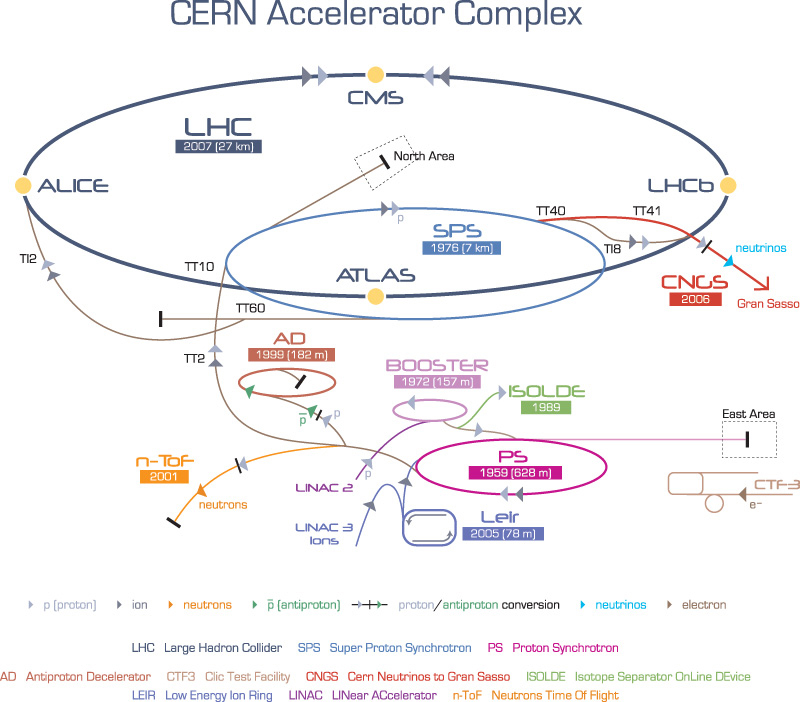
\includegraphics[width=\textwidth]{Bilder/CERNKomplex.jpg}
  \subcaption[Schematische Darstellung von Experimenten am CERN]{Schematische Darstellung verschiedener Experimente am CERN. Für diese Arbeit ist von besonderem Interesse der ATLAS Detektor, welcher an einem Kreuzungspunkt für Proton-Proton Kollisionen am LHC angesiedelt ist \cite{CERNKomplex}.}
  \label{CERNKomplex}
  \end{subfigure}
\begin{subfigure}[t]{0.7\textwidth}
 \includegraphics[width=1\textwidth]{Bilder/Koordinatensystem.pdf}
  \subcaption[Definition des globalen Koordinatensystems von ATLAS]{Das globale Koordinatensystem für den ATLAS Detektor. Die $z$-Achse verläuft parallel zur Strahlachse. $\phi$ als Azimutalwinkel ist in der $x$-$y$-Ebene definiert und die Pseudorapidität $\eta\equiv -\ln\tan{\theta/2}$ ist über den Polarwinkel $\theta$ festgelegt \cite{ATLAS}.}
  \label{Koordinatensystem}
\end{subfigure}
\caption[Schematischer Überblick von Experimenten am CERN und das bei ATLAS festgelegte Koordinatensystem.]{}
\label{CERNKomplexUNDKoordinatensystem}
\end{figure}

Hauptbestandteil des CERN ist der Teilchenbeschleuniger-Komplex innerhalb dessen der Large Hadron Collider (LHC) den größten Ring mit $27\,\text{km}$ Umfang in der Beschleunigerkette darstellt. In diesem werden an vier Kreuzungspunkten Protonpakete zur Kollision gebracht und mit Hilfe von Detektoren die Kollisionsprodukte detektiert. Abb. \ref{CERNKomplex} zeigt schematisch verschiedene Beschleunigerkomponenten und angegliederte Experimente, die Teil des CERN Beschleunigerkomplexes sind und jeweils für ihre jeweiligen Einsatzgebiete optimiert sind.
Das am ATLAS Detektor verwendete Koordinatensystem ist in Abb. \ref{Koordinatensystem} gezeigt und wird so im Laufe der Arbeit verwendet. Der Ursprung wird im Interaktionspunkt (IP) festgelegt. Die $z$-Achse verläuft entlang der Strahlachse und senkrecht dazu liegt die $x$-$y$-Ebene. Der Azimutalwinkel $\phi$ ist als Winkel um die Strahlachse herum definiert und der Polarwinkel $\theta$ misst die Abweichung von der Strahlachse. Die Pseudorapidität ist als $\eta\equiv -\ln\tan{\theta/2}$ definiert. Der Transversalimpuls $p_T$ ist in der $x$-$y$-Ebene definiert \cite{ATLAS}.\\ 
Das Design des Detektors ist in Abbildung \ref{ATLASDesign} aufgezeigt. ATLAS ist zylindersymmetrisch ausgehend vom Interaktionspunkt aufgebaut und sein Magnetsystem be\-steht aus einem supraleitenden Solenoid-Magneten für den inneren Detektor, welches eine Feldstärke von $2\,$T bereitstellt, und aus drei supraleitenden Toroidmagneten, die um die Kalorimeter angeordnet sind. Diese rufen mit ihrem Magnetfeld eine Lorentzkraft hervor und krümmen so die Spur geladener Teilchen, sodass daraus der Transversalimpuls bestimmt werden kann \cite{ATLAS}.\\
\begin{figure}[htbp]                                 
  \begin{center}                                       
  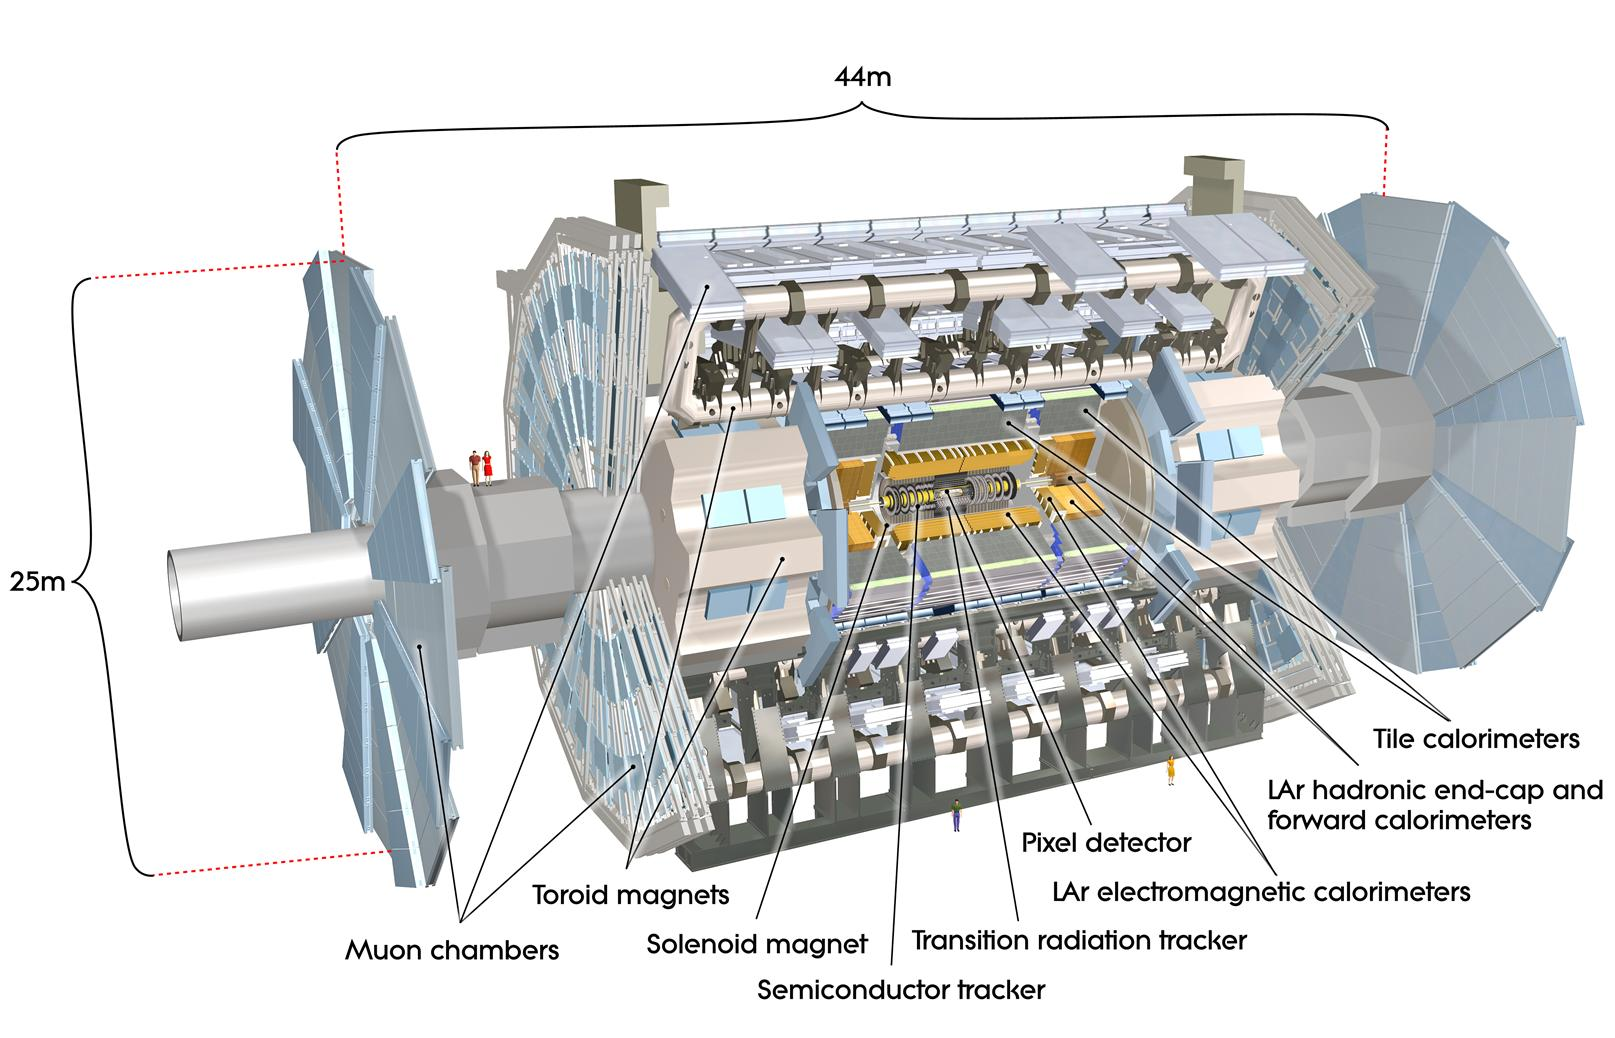
\includegraphics[width=0.8\linewidth]{Bilder/ATLASDesign.png} 
   \caption[Schematische Darstellung des ATLAS Detektors]{Schematische Darstellung des ATLAS Detektors mit seinen Komponenten wie die Myonkammern, Kalorimeter und Magnetspulen sowie Subdetektoren des inneren Zylinderbereichs. \cite{ATLAS}.}
   \label{ATLASDesign}                                     
   \end{center}
\end{figure}
Mithilfe von Halbleiter Pixeldetektoren, Streifendetektoren (SCT) und Über\-gangs\-strahlungs\-de\-tek\-to\-ren (TRT) wird die Teilchenidentifikation, das Ermitteln des Impulses über die Saggitamessung und das Erkennen von Elektronen ermöglicht. Dabei decken die Pixeldetektoren und SCTs einen Bereich von $|\eta|<2,5$, ab während eine Rekonstruktion der Spur mit den TRTs bis zu $|\eta|=2,0$ möglich ist \cite{ATLAS}.\\
Die elektromagnetischen Schichtkalorimeter (EM) -- auf Basis von flüssigen Argon (LAr) und Blei als Absorber -- ermöglichen eine gute Energie- und Ortsauflösung für das Vermessen von Photonen und Elektronen. Das EM ist in zwei Endkappenkomponenten für die Abdeckung der Bereiche $1,375<|\eta|<3,2$ und einen Rumpfteil für die Abdeckung des Bereichs $|\eta|<1,475$ unterteilt. Neben dem  EM existieren hadronische Kalorimeter zur Energiemessung der aus der Kollision resultierenden hadronischen Teilchen. Dabei sind bei ATLAS sowohl hadronische Kalorimeter auf Basis von LAr als aktives Detektormaterial als auch auf Basis von Szintillatortechnik verbaut. Das Szintillator-Kalorimeter mit Blei als Absorbermaterial deckt mit dem zentralen Teil die Region $|\eta|<1,0$ ab und mithilfe seiner Erweiterung die Region $0,8<|\eta|<1,7$. Das ebenfalls auf LAr basierte hadronische Kalorimeter wird als hadronisches Endkappen-Kalorimeter bezeichnet und deckt die Region $1,5<|\eta|<3,2$ ab. Das Vorwärtskalorimeter, welches direkt im Endkappenkryostaten integriert ist, erfüllt die Anforderungen zur elektromagnetischen Messung (Kupfer als Absorbermaterial) und gleichzeitig Energiemessungen von hadronischen Interaktionen (Wolfram als Absorbermaterial) \cite{ATLAS}.\\
Eine weitere wichtige Komponente des ATLAS Detektors stellt das Myon\-spek\-tro\-me\-ter dar, welches für die Messung der Impulse von hochenergetischen Myonen entworfen wurde. Dabei werden zwei Arten von Präzisionskammern zur Spurrekonstruktion eingesetzt -- Monitored Drift Tubes (MDT) und Cathode Strip Chamber (CSC). Resistive Plate Chambers (RPC) und Thin Gap Chambers (TGC) stellen die Komponenten des Triggersystems dar. Das Magnetfeld des Myonsystems wird dabei von den drei Toroidmagneten erzeugt. Das nachfolgende Kapitel \ref{Myonspec} beschreibt das Myonspektrometer mit mehr Details \cite{ATLAS}.\\
Als letztes sei im Rahmen dieses Kapitels noch das Triggersystem von ATLAS angesprochen. Dieses reduziert die Datenrate, welche aufgrund der Kollisionsrate von etwa $1\,$GHz im Detektor erzeugt wird, auf eine Rate von etwa $200\,$Hz. Diese Datenreduktion wird dabei in 3 Stufen erreicht und filtert die physikalisch interessanten Vorgänge für die spätere Rekonstrukion und anschließender Datenanalyse heraus \cite{MS}.  
%%%%%%%%%%%%%%%%%%%%%%%%%%%%%%%%%%%%%%%%%%%%%%%%%%%%%%%%%%%%%%%%%%%%%%%%%%%%%%%%%%%%%%%%%%%%%%%%%%%%%%%%%%%%%%%%%%%%%%%%%%%%%%%
\section{Myonspektrometer und Messung hochenergetischer Myonen}\label{Myonspec}%%%%%%%%%%%%%%%%%%%%%%%%%%%%%%%%%%%%%%%%%%%%%%%%
Mit zunehmendem (Transversal-)Impuls $p$ der Myonen nimmt der Krümmungradius $\rho$ im Magnetfeld $B$ gemäß der Lorentzkraft $\rho\propto p$ weiter zu. Ein größerer Krümmungsradius ist gemäß $\rho=L/\alpha$ in einen Ablenkwinkel $\alpha$ übersetzbar (Magnetlänge $L$)  und wird entsprechend kleiner und damit schlechter messbar, weswegen insgesamt die Rekonstrukion der Myonen schlechter wird. Es gilt für die Auflösung der Impulse: $\sigma_p/p=\sigma_{\alpha}/\alpha$ \cite{Halzen}. 
\begin{figure}[htbp]                                 
  \begin{center}                                       
  \includegraphics[width=0.65\linewidth]{Bilder/MyonSpectrometer.png} 
   \caption[Schematische Darstellung des Myonspektrometers von ATLAS]{Eine schematische Darstellung des Myonspektrometers von ATLAS mit seinen vier verschiedenen Subdetektortypen MDT und CSC (Präzisionskammern) und den Triggerkammern RPC und TGC \cite{ATLAS}.}
   \label{MyonSpectrometer}                                     
   \end{center}
\end{figure}
Deshalb wurde der ATLAS Detektor so konstruiert, dass mit dem Myonspektrometer die Möglichkeit besteht, eine zweite Impulsmessung der Myonen durchzuführen, die für hohe Transversalimpulse ($\mathcal{O}(100\,\text{GeV})$) optimiert ist.\\
Wie in Kapitel \ref{ATLAS} erwähnt, besteht das Myonspektrometer aus vier verschiedenen Typen von Gasdetektoren. Zwei Detektortypen -- MDT und CSC -- sind Prä\-zisions\-kammern zur genauen Spurrekonstruktion der Myonen, während RPC und TGC für das Triggersystem verwendet werden. Abb. \ref{MyonSpectrometer} zeigt schematisch den Aufbau des Myonspektrometers mit den jeweiligen Detektorkomponenten. 

MDTs nehmen mit $5500\,$m$^2$  die größte aktive Fläche ein und werden in den großen Rädern und im Rumpf des Detektors eingesetzt (s. Abb. \ref{MyonSpectrometer}). Das Prinzip der MDTs ist das einer Driftröhre, die zur Detektion von Teilchen die Gasverstärkung (Verstärkungsfaktor von $2\cdot10^4$) nutzt. Das verwenete Gas ist ein Gemisch aus Argon, Stickstoff und Methan. Das Drahtmaterial der Aluminium-Driftröhre besteht aus einer Wolfram-Rhenium Legierung und liegt auf einem elektrischen Potenzial von $3,3\,$kV. Für perfekte Ausrichtung und damit genaue Messung der Transversalimpulse mit den Driftröhren, wird eine optisches Kontrollsystem verwendet, welches die mechanischen Verschiebungen der Module überwacht. CSCs ergänzen das System der Präzisionskammern (Abb. \ref{MyonSpectrometer}) im Pseudorapiditätsbereich $2,0<|\eta|<2,7$ wegen der größeren Beständigkeit gegen hohen Teilchenraten, die besonders in diesem Be\-reich des Detektors vorherrschen. CSCs sind Drahtkammern mit mehreren Anodendrähten die sich zwischen zwei parallelen Kathoden befinden. Der Freiraum ist ebenfalls mit einem Gasgemisch (bei CSCs: Argon-Kohlenstoffdioxid-Tetrafluormethan) gefüllt, sodass beim Durchgang eines Teilchens das Gas ionisiert wird und eine Gasverstärkung von $1\cdot10^4$ das entsprechende Messsignal liefert. Dabei liegen die Wolfram-Rhenium Drähte auf einem Potenzial von $2,6$kV. Werden dabei Streifen\-ka\-thoden verwendet, so lässt sich eine Ortsauflösung erzielen, die hier bei $60$µm liegt. Die Zeitauflösung beträgt $7$ns \cite{MS}.

Dem Anspruch an eine hohe Zeitauflösung für das Triggersystem tragen im Falle des ATLAS Detektors die Widerstandsplattenkammern (RPC) und die TGCs Rechnung. RPC sind ebenfalls Gasdetektoren und basieren auf dem das Prinzip der Gasverstärkung (RPC Gemisch: Tetrafluorethan-Butan) zwischen zwei Kupferelektroden. Hochohmige Bakelitplatten\footnote{Bakelit ist ein aus Polykondensation gewonnener Kunststoff auf Basis von Phenol und Formaldehyd \cite{Bakelit}.} sind vor den Kathoden angeordnet, sodass nur Gasentladungseffekte bei einer Betriebsspannung von $8,9$kV anulliert werden. Die Zeitauflösung beträgt $1,5$ns. RPCs im ATLAS Detektor decken den Bereich $|\eta|<1,05$ ab. Die zweite Triggerart, TGCs, sind in der Region $1,05<|\eta|<2,7$ verbaut und sind vom Prinzip wie eine Vielfachdrahtkammer aufgebaut. Das unterscheidende Merkmal ist jedoch der Abstand zwischen den Anoden, welcher größer als der Kathoden-Anoden Abstand ist. Außerdem befinden sich die Drähte auf einem elektrischen Potenzial von $3,1$kV. Dies erlaubt eine zeitliche Auflösung mit $>99\%$iger Effizienz bei Betrieb mit einem Kohlenstoffdioxid-n-Pentan-Gasgemisch \cite{MS}\cite{PhysTeV}.

%Optional noch das Triggerschema:
%ATLAS besitzt ein dreistufiges Triggerschema: Level 1 Trigger reduziert die Datenrate von $40\,$MHz, was der Kollisionsrate entspricht, auf eine Niveau von $75-1000\,$kHz. Dabei markiert der Level 1 Trigger Ereignisse von besonderem Interesse (die sogenannten Regions of Interest). Die Level 2 Trigger wählen aus den Regions of Interest mit gesamter Detailgenauigkeit und voller Präzision aus und können somit die Datenrate auf $2$kHz reduzieren. Die Trigger der Stufe 3, auch als Eventfilter genannt, liefern dann eine Ausgaberate von $200$Hz. In diesem Schritt wird die offline Beurteilung durchgeführt und beispielsweise  
%
\begin{figure}[htbp]                                 
  \begin{center}                                       
  \includegraphics[width=0.6\linewidth]{Bilder/Myontypen.pdf} 
   \caption[Verschiedene Myontypen, die sich bei der Spurrekonstruktion bei ATLAS ergeben können]{Je nach Signaturen in den verschiedenen Subdetektoren ergeben sich unterschiedliche Myontypen \cite{Verena}.}
   \label{Myontypen}                                     
   \end{center}
\end{figure}
Für das spätere Verständnis soll in diesem Abschnitt die verschiedenen Myontypen\footnote{Myontyp ist in diesem Zusammenhang so zu verstehen, dass es verschiedene Arten der Myonrekonstruktion gibt, die möglichst gut das physikalische Objekt Myon widerspiegeln sollte.} erklärt werden. Abhängig davon, welche Detekorsysteme für die Rekonstruktion der Myonen verwendet wurden, lassen sich die Myonen in verschiedene Typen einteilen (s. dazu Abb. \ref{Myontypen}).
\textbf{Combined muons} (CB) sind Myonen, deren Spur unabhängig aus Treffern im inneren Detektor und im Myonspektrometer re\-kon\-stru\-iert und kombiniert wird. \textbf{Segment-tagged muons} (ST) sind Myonen, bei denen eine Spur aus dem inneren Detektor als Myon identifiziert wird, und eine Extrapolation zum Myonspektrometer eine Übereinstimmung mit einem Spursegment im Myonspektrometer ergibt. Dies betrifft Myonen mit niedrigen Impulsen, welche deshalb keine weiteren Segmente treffen. \textbf{Calorimeter-tagged muons} (CT) werden zusammen mit einer Spur im inneren Detektor und einer passenden Energiedeposition im Kalorimeter identifiziert. Als letzter Myontyp dieser Aufzählung existiert das \textbf{Extrapolated Muon} (ME), dessen Spur allein durch das Myonspektrometer rekonstruiert wird und für das lockere Bedingungen bezüglich der Kompatibilität mit dem Spurursprung im Interaktionspunkt gefordert werden \cite{MuPerNeu}.
% 
%
%Segmenten Barrel Inner Small 7 erlären
%
%%%%%%%%%%%%%%%%%%%%%%%%%%%%%%%%%%%%%%%%%%%%%%%%%%%%%%%%%%%%%%%%%%%%%%%%%%%%%%%%%%%%%%%%%%%%%%%%%%%%%%%%%%%%%%%%%%%%%%%%%%%%%%%
\section{Leptoquark-Produktion in Proton-Proton Kollisionen}\label{LQpp}%%%%%%%%%%%%%%%%%%%%%%%%%%%%%%%%%%%%%%%%%%%%%%%%%%%%%%%
Für die Suche nach Leptoquarks mithilfe des ATLAS Detektors (s. Kapitel \ref{ATLAS}) werden aufbauend auf das BRW Modell (s. Kapitel \ref{LQ}) noch zwei weitere Annahmen getroffen:\\
Jedes Leptoquark soll nur an eine bestimmte Generation von Leptonen und Quarks koppeln. Dies ist eine zusätzliche Annahme, da im BRW Modell Leptoquarks prinzipiell in alle möglichen Kombinationen zerfallen können. Die zweite Annahme schreibt rein chirale Wechselwirkungen mit den Fermionen des Standardmodells vor.\\
Diese beiden Bedingungen komprimieren das BRW Modell zum minimalen-Buchmüller-Rückl-Weyler-Modell (mBRW) \cite{Kuze}, welches Leptoquarkmassen in Reichweite der heutigen Teilchenbeschleuniger zulässt. %Ein weiterer Grund für die Annahmen des mBRW Modells liegt in Flavour-Changing-Neutral Currents, die ohne das mBRW vermehrt auftreten würden, (bei der Massengrößenordnung) was experimentell nicht beobachtet wird und theoretisch der GIM Mechanismus unterdrückt. %So, hier muss noch viel getan weden: soll das rein, dann ein paar worte über flavour cnc und GIM verlieren + referenzieren%-->mBRW siehe LQATLAS als REFERENZ
Innerhalb des mBRW Modells, was nun als Grundlage für diese Suche nach Leptoquarkpaaren am ATLAS Detektor dienen soll, sind dann die Hauptprozesse der Leptoquarkproduktion Quark-Antiquark Vernichtung und Gluon-Fusion in führender Ordnung. Abb. \ref{LQProduction} zeigt diese Prozesse anhand von Feynmandiagrammen \cite{LQATLAS}.   
\begin{figure}[htbp]                                 
  \begin{center}                                       
  \includegraphics[width=0.3\linewidth]{Bilder/LQProduction.jpeg} 
  \includegraphics[width=0.3\linewidth]{Bilder/LQProduction2.jpeg}\\ 
  \includegraphics[width=0.3\linewidth]{Bilder/LQProduction3.jpeg}
  \includegraphics[width=0.3\linewidth]{Bilder/LQProduction4.jpeg}
   \caption[Feynmandiagramme führender Ordnung für die Leptoquark-Paar-Produktion durch Quark-Antiquark-Vernichtung und Gluon-Fusion in Proton-Proton Kollisionen]{Feynmandiagramme führender Ordnung für die Leptoquark-Paar-Produktion durch Quark-Antiquark-Vernichtung und Gluon-Fusion in Proton-Proton Kollisionen \cite{LQATLAS}.}
   \label{LQProduction}                                     
   \end{center}
\end{figure}
Detektierbare Endzustände resultieren dann aus der Zerfallscharakteristik der in Proton-Proton-Kollisionen erzeugten Leptoquarkpaare. Nach dem mBRW Modell sind das im Einzelnen \cite{Schrempp}:
\begin{align}
  LQ_1\rightarrow u\overline{\nu}_e, de^+&\qquad \overline{LQ}_1\rightarrow \overline{u}\nu_e, \overline{d}e^-\\
  LQ_2\rightarrow c\overline{\nu}_\mu, s\mu^+&\qquad \overline{LQ}_2\rightarrow \overline{c}\nu_\mu, \overline{s}\mu^-\label{2. GenLQ}\\
  LQ_3\rightarrow t\overline{\nu}_\tau, b\tau^+&\qquad \overline{LQ}_3\rightarrow \overline{t}\nu_\tau, \overline{b}\tau^-
\end{align}
In dieser Arbeit soll aber der Fokus auf den Zerfall von Leptoquarkpaaren in zweiter Generation gerichtet sein, woraus der Endzustand µµjj, also Myonen µ und Jets j, hervorgeht (s. Gl. \ref{2. GenLQ}).
%%%%%%%%%%%%%%%%%%%%%%%%%%%%%%%%%%%%%%%%%%%%%%%%%%%%%%%%%%%%%%%%%%%%%%%%%%%%%%%%%%%%%%%%%%%%%%%%%%%%%%%%%%%%%%%%%%%%%%%%%%%%%%%
\chapter{Datenanalyse}%%%%%%%%%%%%%%%%%%%%%%%%%%%%%%%%%%%%%%%%%%%%%%%%%%%%%%%%%%%%%%%%%%%%%%%%%%%%%%%%%%%%%%%%%%%%%%%%%%%%%%%%%
Der aktuelle Stand für die Suche nach skalaren Leptoquarks der zweiten Generation und die grundlegenden Auswahlkriterien und Bedingungen, welche für die Datenanalyse im Falle der Leptoquarks erfüllt sein müssen, sollen in diesem Kapitel beschrieben werden. Darauf aufbauend wird das Ziel dieser Arbeit mit den jeweiligen Arbeitsschritten dargelegt und im Hauptteil folgen die erzielten Ergebnisse.
%%%%%%%%%%%%%%%%%%%%%%%%%%%%%%%%%%%%%%%%%%%%%%%%%%%%%%%%%%%%%%%%%%%%%%%%%%%%%%%%%%%%%%%%%%%%%%%%%%%%%%%%%%%%%%%%%%%%%%%%%%%%%% 
\section{Derzeitiger Stand in der Suche nach skalaren Leptoquarks}\label{derzeitigerStand}%%%%%%%%%%%%%%%%%%%%%%%%%%%%%%%%%%%%%
Dieses Kapitel soll einen kurzen Überblick über den derzeitigen Stand für die Suche nach skalaren Lepoquarks mit dem ATLAS Detektor geben. Dabei soll im Rahmen dieser Arbeit vor Allem auf Leptoquarks der zweiten Generation nach dem minimalen-Buchmüller-Rückl-Weyler-Modell (mBRW)\footnote{Für das minimal-Buchmüller-Rückl-Weyler-Modell siehe Kapitel \ref{LQpp}} eingegangen werden.

Für die Suche nach skalaren Leptoquarks spielt die Ereignisselektion eine der grundlegensten Rollen. Hierfür wurden die ATLAS Daten aus Run 2 des Jahres 2015 bei einer Schwerpunktsenergie $\sqrt{s}=13\,\text{TeV}$\footnote{$s$ ist dabei eine der drei Mandelstam Variablen $s$, $t$ und $u$ \cite[S. 94]{Halzen}.} verwendet. Nach Anwendung aller Qualitätskriterien behält der verwendete Datensatz eine integrierte Luminosität von $\mathcal{L}=3{,}2\,\text{fb}^{-1}$. Für die Suche nach µµjj Signaturen, wenn µ das Myon bezeichnet und j einen Jet, wird eine Triggerschwelle in Level 1 für den Transversalimpuls des Myons von $p_T\geq 26\,\text{GeV/c}$ verwendet und zusätzlich ein isoliertes Myon gefordert. Der Level 2 Trigger verwendet eine Schwelle von $p_T\geq 50\,\text{GeV/c}$ ohne zusätzlichen Bedingungen \cite{LQATLAS}.%Absatz Datensatz und Eventmodell

Die Myonrekonstruktion bei der Suche nach skalaren Leptoquarks basiert auf der unabhängigen Spurrekonstruktion der Myonen im inneren Detektor und im Myonspektrometer, jeweils mit einer bestimmten Anzahl von Signaturen in einer Kammer (Hits) und geometrischen Kriterien. Für die Analyse wird eine Kombination der beiden unabhängigen Spurrekonstruktionen aus dem Inner Detector und dem Myonspektrometer und unter Berücksichtigung von Energieverlust im Kalorimeter und Vielfachstreuung der Myonen verwendet. Die verlässliche Messung von Myonen mit Transversalimpulsen größer $100\text{GeV}/\text{c}$ fordert drei Treffer in mindestens drei Präzisionskammern. Die q/p Signifikanz wird ebenfalls unabhängig im inneren Detektor und im Myonspektrometer gemessen und anschließend kombiniert. Die Übereinstimmung muss innerhalb sieben Standardabweichungen gegeben sein. Forderungen für den Transversalimpuls von $p_T\geq40GeV/c$ und die Pseudorapidität von $|\eta|\leq2{,}5$ werden zusätzlich aufgestellt, weil dieser Bereich der Pseudorapidität die Abdeckung des inneren Detektors widerspiegelt. Aufgrund des nicht bestimmbaren Versatzes\footnote{Kapitel \ref{passedHighPtCuts Funktion} liefert in einer genaueren Betrachtung die Begründung, weshalb der Versatz zu Problemen in der Transversalimpulsauflösung führen kann und somit ausgeschlossen wird.} von Zylinder- und Endkappenberich des ATLAS Detektors werden die Regionen $1{,}01\leq|\eta|\leq1{,}10$ mit einem Veto versehen. Für die Stoßparameter $d_0$ und $z_0$ wird $|\frac{d_0}{\sigma_{d_0}}|\leq3$ und $|z_0\sin\theta|\leq0{,}5\,\text{mm}$ gefordert. Außerdem werden Restriktionen in der Isolation mit $\Delta R=10\frac{\text{GeV}}{\text{c}}/p_T^\mu$\footnote{Dabei ist $\Delta R=\sqrt{\Delta\eta^2+\Delta\phi^2}$ ein Kegel, der durch die Differenz in Pseudorapidität $\Delta\eta$ und Azimutalwinkel $\Delta\phi$ definiert ist (vgl. \cite{LQATLAS}).} auferlegt \cite{LQATLAS}.%physics object definition Absatz
\begin{figure}
  \begin{subfigure}[t]{0.4\textwidth}
  \includegraphics[width=\textwidth]{Bilder/DY+Jets.pdf}
  \subcaption{}
  \label{DY+Jets}
  \end{subfigure}
\begin{subfigure}[t]{0.4\textwidth}
  \includegraphics[width=\textwidth]{Bilder/ttbar.pdf}
  \subcaption{}
  \label{ttbar}
\end{subfigure}
\begin{subfigure}[t]{0.4\textwidth}
  \includegraphics[width=\textwidth]{Bilder/Wt.pdf}
  \subcaption{}
  \label{Wt}
\end{subfigure}
$\hfill$
\begin{subfigure}[t]{0.4\textwidth}
  \includegraphics[width=\textwidth]{Bilder/Ztautau.pdf}
  \subcaption{}
  \label{Ztautau}
\end{subfigure}
\caption{Beispiele für die in der Suche nach skalaren Leptoquarks berücksichtigten Untergründe (a) DY+Jets, (b) $t\bar{t}$, (c) W$t$ und des Zerfalls eines (d) Z$^0$ Bosons in zwei Tauonen anhand eines Feynmandiagramms.}
\end{figure}

Die Analysestrategie zur Identifikation von Signalereignissen beruht auf der Sei\-ten\-band-Methode mit den verschiedenen Regionen (Signalregion, Kontrollregion, Validierungsregion). Die Variablen, anhand denen der Unterschied zwischen Untergrund und Signal unterschieden werden, sind die invariante Zwei-Leptonmasse $m_{ll}$ und die skalare Summe $S_T$ der Transversalimpulse der beiden Leptonen und der beiden Jets sowie die minimale Leptoquarkmasse $m_{\text{min}}^{LQ}$. Letztere Variable ergibt sich dabei aus folgender Überlegung: Die Endprodukte Myon µ und Jet j aus dem Zerfall der Leptoquarkpaare (wie in Kap. \ref{LQpp} beschrieben) werden jeweils zu $m_{ij}^{LQ}$ gepaart. Dabei werden alle Kombinationen aus $\mu_i$ und $j_j$ berücksichtigt. Somit erhält man entsprechend $m_{11}^{LQ}$, $m_{22}^{Lq}$, $m_{12}^{LQ}$ und $m_{21}^{LQ}$. Die kleinere Differenz der Masse von $\Delta m_{1}^{LQ}=|m_{11}^{LQ}-m_{22}^{LQ}|$ und $\Delta m_{2}^{LQ}=|m_{12}^{LQ}-m_{21}^{LQ}|$ ist die Paarung der Wahl. Anschließend wird aus der kleineren Massendifferenz das Paar $m_{ij}^{LQ}$, welches die kleinere Masse trägt, als $m_{\text{min}}^{LQ}$ definiert. Die Wahl der Signalregion fällt auf den Bereich $m_{ll}\geq130\,\text{GeV}/\text{c}^2$ und $S_{T}\geq600\,\text{GeV}/\text{c}$, wobei Schnitte in der invarianten Zwei-Leptonmasse $m_{ll}$ und in $S_{T}$ so optimiert sind, dass Untergrundprozesse reduziert werden ohne zu viel Signal zu verlieren. Die sich nicht überlappenden Kontrollregionen dienen der Normierung der Monte Carlo Vorhersagen für die Hintergründe durch Drell-Yan-Prozesse\footnote{Zur Erklärung von Drell-Yan Prozessen siehe nächsten Absatz in der Auflistung der Untergrundprozesse.} zusammen mit Jets und durch $t\bar{t}$ Untergrundprozesse. Die Validierungsregion dient dazu, die Übereinstimmung von Monte Carlo Simulation mit den Daten zu prüfen unter der gleichzeitigen Bedingung, wenig Signalkontamination in der Validierungsregion zu haben. Das lässt sich durch eine Invertierung des Schnittes in $S_T$ erreichen.%Absatz CR;VR;SR 
\begin{figure}[htbp]                                 
  \begin{center}                                       
  \includegraphics[width=0.5\linewidth]{Bilder/VRLQMass.pdf} 
   \caption[Die minimale invariante Masse des rekonstruierten Leptoquarks zweiter Generation in den zwei Validierungsregionen]{Die minimale invariante Masse des rekonstruierten Leptoquarks zweiter Generation (µµjj) $m_{\text{min}}^{LQ}$ in den zwei Validierungsregionen für die vorhergesagten Untergründe im Vergleich zu den mit ~ATLAS gemessenen Daten \cite{LQATLAS}.}
   \label{VRLQMass}                                     
   \end{center}
\end{figure}

Bei der Untergrundbetrachtung in der Analyse sind folgende Prozesse berücksichtigt \cite{LQATLAS}:
\begin{itemize}
    \item Drell-Yan-Prozesse zusammen mit Jets (DY+Jets): Hier wird der inelastischen Partonstreuung Rechnung getragen. Bei der Quark-Antiquark Vernichtung werden virtuelle Photonen oder Z$^0$ Bosonen erzeugt, welche wiederum in ein Leptonpaar $l\bar{l}$ (also beispielsweise in ein $\mu^-\mu^+$) zerfallen. Dabei kann für höhere Korrekturen der Wechselwirkung auch Gluon-Bremsstrahlung auftreten, die für die Produktion von Jets verantwortlich sind. Ein Feynmangraph für einen DY+Jet Prozess ist in Abb. \ref{DY+Jets} gezeigt \cite{PhysTeV}. 
    \item Topquark-Antitopquark Untergründe: Über Quark-Antiquark-Vernichtung oder Gluonfusion lässt sich bei Proton-Proton Kollisionen Top-Antitop-Quarkpaare erzeugen, die bei ihrem Zerfall über ein Bottomquark und W$^\pm$ Bosonen zu\-sätz\-lich Leptonen (hier Myonen) und Jets als Untergrund erzeugen. Beispielhaft ist in Abb. \ref{ttbar} ein Feynmangraph für solch einen Untergrundprozess gezeigt \cite{PhysTeV}.
    \item Kleinere Beiträge aus dem Wt-Kanal und der Zerfall von einem Z$^0$ Boson in zwei Tauonen: Durch beispielsweise eine Quark-Antiquark-Vernichtung lässt sich über ein W$^\pm$ Boson ein einzelnes Topquark mit einem Antibottom erzeugen, welches dann wie in der vorherigen Aufzählung entsprechend weiter in Leptonen und ein Bottomquark zerfallen kann und somit weiteren Untergrund hinzufügt (siehe Feynmandiagramm in Abb. \ref{Wt}). Eine weitere Untergrundquelle ist die Produktion von einem Z$^0$, welches in zwei Tauonen zerfällt und anschließend weiteren leptonischen Untergrund erzeugt. Dies zeigt das Feynmandiagramm in Abb. \ref{Ztautau}. 
\end{itemize}%Untergrundbetrachtung

Die Analyse liefert folgende Ergebnisse: Die Ergebnisse der Analyse stimmen mit den Erwartungen aus dem Standardmodell überein. Die extrapolierte Untergrundvorhersage der Kontrollregion konnte durch die Validierungsregion bestätigt werden. Die Verteilung der minmalen invarianten Leptoquarkmasse $m_{\text{min}}^{LQ}$ in den zwei Validierungsregionen ist in Abb. \ref{VRLQMass} im Vergleich zum Untergrund gezeigt und stimmt im Rahmen der Unsicherheiten mit den gemessenen Daten überein. Auch für die erwarteten Ereignisse im µµjj Kanal in Signalregion und den beiden Kontrollregionen im Vergleich zu den beobachteten Raten lässt sich keine signifikante Abweichung von den Vorhersagen des Standardmodells feststellen. Die beobachtete Massenverteilung von $m_{\text{min}}^{LQ}$ in der Signalregion ist in Abb. \ref{SRLQMass} gezeigt. Dabei ist das Vergleichskriterium die Untergrundvorhersage auf Grundlage einer kombinierten Kurvenanpassung in der Kontroll- und Signalregion. Im Rahmen des Fehlers sind die Daten mit dem Untergrund nach dem Standardmodell vereinbar und zeigen keine signifikante Abweichungen \cite{LQATLAS}.%Results
\begin{figure}[htbp]                                 
  \begin{center}                                       
  \includegraphics[width=0.5\linewidth]{Bilder/SRLQMass.pdf} 
   \caption[Die minimale invariante Massenverteilung des rekonstruierten Leptoquarks zweiter Generation in der Signalregion]{Die minimale invariante Massenverteilung des rekonstruierten Leptoquarks zweiter Generation (µµjj) $m_{\text{min}}^{LQ}$ in der Signalregion im Vergleich zu den vorhergesagten Untergründen nach dem Standardmodell \cite{LQATLAS}.}
   \label{SRLQMass}                                     
   \end{center}
\end{figure}
%Hier könnte jetzt noch was zu bracnhing ratio * cross section plot stehen
Auf Grundlage dieses aktuellen Stands soll im nachfolgenden Kapitel \ref{AusgangspunktProblemstellung} erklärt werden, an welchem Punkt die Analyse dieser Arbeit an\-setzt. 
%%%%%%%%%%%%%%%%%%%%%%%%%%%%%%%%%%%%%%%%%%%%%%%%%%%%%%%%%%%%%%%%%%%%%%%%%%%%%%%%%%%%%%%%%%%%%%%%%%%%%%%%%%%%%%%%%%%%%%%%%%%%%%%
\section{Ausgangspunkt und Aufgabenstellung der Analyse}\label{AusgangspunktProblemstellung}%%%%%%%%%%%%%%%%%%%%%%%%%%%%%%%%%%%
Nach den Suchkriterien für skalare Leptoquarks wie in Kapitel \ref{derzeitigerStand} beschrieben, konnte festgestellt werden, dass die gemessenen Daten im Rahmen der Unsicherheiten mit den Erwartungen des Standardmodells übereinstimmen. Unter den beschriebenen Annahmen in Kapitel \ref{LQpp} nach dem mBRW Modell sind Massenlimits der Leptoquarks bestimmt worden. Demnach bestehen Massenlimits von $1050\text{GeV}/\text{c}^2$ für die zweite Generation Leptoquarks auf der Grundlage eines $95$\% Konfidenzniveaus unter der Annahme, dass das Vezweigungsverhältnis der Leptoquarks $\beta=1$ beträgt. 
\begin{table}[htbp]
		\centering
		\begin{tabular*}{0.4\linewidth}{cc|c}
		\hline
		\hline
		\rule[7pt]{0pt}{23pt} $m_{LQ} [\text{TeV}/\text{c}^2]$ & \multicolumn{2}{c}{$\epsilon [\%]$}  
		\\
		\cline{2-3}
		\rule[-7pt]{0pt}{23pt} & eejj & µµjj
		\\
		\hline
		\rule[-6pt]{0pt}{21pt} $0{,}50$ & \(60{,}9\) & $42{,}4$ 
		\\
		\rule[-6pt]{0pt}{21pt}$0{,}75$&  \(68{,}9\)	& $45{,}8$ 
		\\
		\rule[-6pt]{0pt}{21pt} $1{,}00$ & \(72{,}3\) & $46{,}0$ 
		\\
		\rule[-6pt]{0pt}{21pt}$1{,}25$ &  \(72{,}6\)	& $45{,}8$ 
		\\
		\rule[-6pt]{0pt}{21pt} $1{,}50$ & \(73{,}2\) & $45{,}0$ 
		\\
		\hline
		\hline
		\end{tabular*}
		\caption[Selektionseffizienzen in den Kanälen eejj und µµjj für unterschiedliche Leptoquarmassen im Vergleich]{Selektionseffizienzen für den eejj Kanal (Leptoquarks erster Generation) und den µµjj (Leptoquarks zweiter Generation) im Vergleich. Dabei sind auch unterschiedliche Massen der Leptoquarks $m_{LQ}$ berücksichtigt (nach \cite{LQATLAS}).}
		\label{SelektionsEffPaper}
	\end{table}

Allerdings geht in diese Analyse %wie genau geht sie jetzt ein?-->dann wieder zu einem Absatz
die Selektionseffizienz der Myonen ein, welche zusammen mit den Jets die Leptoquarks zweiter Generation rekonstruieren. Betrachtet man Tab. \ref{SelektionsEffPaper}, so erkennt man die um den Faktor $1{,}5$ niederigere Selektionseffizienz für Myonen im Vergleich zur Selektionseffizienz für Elektronen. Diese systematisch niedrigeren Effizienzen bei Myonen liegt an den hohen Anforderungen für die Spurmessung hochenergetischer Myonen (s. Kap. \ref{Myonspec}) \cite{LQATLAS}. Um nun eine Möglichkeit der Optimierung zu eröffnen, soll in dieser Arbeit untersucht werden, welche Einflüsse Selektionensmaßnahmen für Myonen auf die Gesamteffizienz haben.\\ %Erster Abschnitt LQ
Im zweiten Schritt werden Monte Carlo Simulationen, bei denen Z$^0$ Bosonen produziert werden und anschließend in zwei Myonen zerfallen, als Kontrolle der obigen Schnittunterteilung verwendet. Die Wahl für einen Z$^0$ Monte Carlo Datensatz liegt darin begründet, dass diese Prozesse sehr gut verstanden und umfangreich analysiert sind. Die Kontrolle wird dabei so gewährleistet, dass auch hier wieder die Effizienzen der einzelnen Selektionen (s. Kap. \ref{einzelneSchnitte}) untersucht werden und mit obigen verglichen werden können. Dazu werden nur Myonpaare verwendet, die auf Basis der Spurmessung des inneren Detektors die Masse des Z$^0$ Bosons $m_{\text{Z}^0}=91\text{GeV}/\text{c}^2$ rekonstruieren. Als Toleranzbereich wird das Intervall $]80\text{GeV}/\text{c}^2\,;\,101\text{GeV}/\text{c}^2[$ (nach \cite[S. 9]{MuPerNeu}) gewählt. Sind mehrere Myonpaare möglich, wird das Paar verwendet, dessen invariante Masse näher an der Z$^0$ Masse liegt. %Zweiter Abschnitt Z s
%%%%%%%%%%%%%%%%%%%%%%%%%%%%%%%%%%%%%%%%%%%%%%%%%%%%%%%%%%%%%%%%%%%%%%%%%%%%%%%%%%%%%%%%%%%%%%%%%%%%%%%%%%%%%%%%%%%%%%%%%%%%%%%
\section{Die Datengrundlage}%%%%%%%%%%%%%%%%%%%%%%%%%%%%%%%%%%%%%%%%%%%%%%%%%%%%%%%%%%%%%%%%%%%%%%%%%%%%%%%%%%%%%%%%%%%%%%%%%%%
Die vorliegende Analyse wurde in RootCore mit der Analysis Base 2.3.45 durchgeführt. RootCore ist eine objektorientierte Programmierumgebung, welche die Ana\-lyse von großen Datensätzen und das Einbinden von ATLAS-weiten Paketen erlaubt. Das verwendete Format, welches die für die Datenanalyse relevanten Informationen der Ereignisse beinhaltet, ist ein DxAOD der Arbeitsgruppe für die Suche nach exotischen Teilchen bei ATLAS.

Datengrundlage für die Untersuchung, welche Effizienzverluste bei einzelnen Selektionsschritten von Myonen bei der Suche nach skalaren Leptoquarks zweiter Generation auftreten, ist ein Monte Carlo Datensatz für die Paarproduktion von Leptoquarks im Massenbereich von $500-1500\,\text{GeV}/\text{c}^2$ nach dem mBRW Modell (siehe Kapitel \ref{LQpp}). Um diesen Datensatz\footnote{Die genaue Bezeichnung für den Leptoquark-Datensatz lautet \nolinkurl{mc15_13TeV.302935.Pythia8EvtGen_A14NNPDF23LO_LQ_cmucmu_1000.merge.DAOD_EXOT12.e4215_a766_a777_r6282_p2419_tid06481986_00/DAOD_EXOT12.06481986._000001.pool.root.1}.} bei einer Schwerpunktsenergie von $\sqrt{s}=13\text{TeV}$ zu erzeugen wurde der Pythia8 Eventgenerator \cite{Pythia8} mit zusätzlichen Feinabstimmungen\footnote{Für weitere Einzelheiten siehe \cite{LQATLAS}} verwendet. Es wurden weitere Simulationen beispielsweise der Untergrundprozesse mit anderen Generatoren miteinbezogen. %Hier vielleict etwas schmu über Eventgeneratoren?

Für den zweiten Analyseteil dieser Arbeit wurden außerdem Monte Carlo Datensätze mit der Entstehung und dem anschließenden  Zerfall Z$^0\rightarrow\mu\mu$ verwendet. Der wesentliche für die Produktion der Z-Datensätze\footnote{Die genaue Bezeichnung für die Z-Datensätze lautet \nolinkurl{mc15_13TeV.361107.PowhegPythia8EvtGen_AZNLOCTEQ6L1_Zmumu.merge.DAOD_MUON1.e3601_s2576_s2132_r6765_r6282_p2421_tid06537915_00/DAOD_MUON1.065379}\texttt{\textcolor{cyan}{15}}\nolinkurl{._0000}\texttt{\textcolor{cyan}{02}}\nolinkurl{.pool.root.1}. Dabei zeigt die farbige Hervorhebung, wo sich die Namen in Abhängigkeit der Datensätze verändern.} verwendete Eventgenerator ist ebenfalls Pythia8 \cite{Pythia8}. Powheg \cite{Powheg} und EvtGen \cite{EvtGen} sind für weitere Feinabstimmungen im Simulationsschritt des Z$^0$ Bosons verantwortlich.
%
%EvtGen simuliert b und c Zerfall
%
%
%%%%%%%%%%%%%%%%%%%%%%%%%%%%%%%%%%%%%%%%%%%%%%%%%%%%%%%%%%%%%%%%%%%%%%%%%%%%%%%%%%%%%%%%%%%%%%%%%%%%%%%%%%%%%%%%%%%%%%%%%%%%%%%
\section{Selektionskriterien für Myonen}\label{Selektionskriterien}
Ein wichtiges Werkzeug der ATLAS-Datenanalyse für die Rekonstruktion von Myonen ist das MuonSelectionTool. Dieses Tool wurde speziell für die verschiedenen Anforderungen bei der Identifikation von Myonen entwickelt und stellt spezifische Arbeitspunkte zur Verfügung, die auf die Daten des ATLAS Experiments von 2013 optimiert sind.\\ 
Es gibt den Arbeitspunkt der \textbf{Medium muons}, welcher der Standard für die Myonselektion bei ATLAS darstellt und dessen Kriterien auf ein Minimieren der systematischen Unsicherheiten bei der Myonrekonstruktion abzielt. Die Identifikation der Myonen nach den Kriterien des Arbeitspunktes \textbf{Loose muons} wurde für das Maximieren der Rekonstruktionseffizienzen bei gleichzeitig guter Qualität der Myonspuren entworfen. Neben dem Arbeitspunkt \textbf{Tight muons}, welcher auf Kosten der Effizienz die Reinheit der Daten erhöht, wird der Arbeitspunkt der \textbf{High-$p_{T}$ muons} verwendet. Da sich diese Arbeit mit hochenergetischen Myonen beschäftigt und dieser Arbeitspunkt bei der Suche nach Leptoquarks verwendet wird, spielt dieser Arbeitspunkt die zentrale Rolle. Dieser Arbeitspunkt wird im Kapitel \ref{einzelneSchnitte} kleingliedriger untersucht, um die Effizienzverluste in den einzelnen Schritten zu identifizieren. Die Auswahl der Myonen nach High-$p_{T}$ muons ist speziell für Myonen mit einem Transversalimpuls größer $100$GeV entworfen, um die Impulsauflösung für Spuren in diesem hochenergetischen Regime zu maximieren. Notwendige Voraussetz\-ung dafür, dass Myonen als high-$p_{T}$ im Sinne der Auswahl eingestuft werden, ist das Erfüllen der Kriterien für den Arbeitspunkt Medium muons. Wichtige Krite\-rien sind dabei, dass CB und ME\footnote{Zur Defintion der Myontypen siehe Kapitel \ref{Myonspec}.} Spuren gefordert werden, wobei CB Myonen mindestens drei Treffer in mindestens zwei MDT Kammern aufweisen müssen, außer die Spur befindet sich in der Region $|\eta|<0{,}1$. Dann muss die Spur mindestens einen Treffer in einer MDT Schicht besitzen und darf nicht mehr als ein MDT Loch\footnote{Verläuft die Spurrekonstruktion eines Myons durch eine Messkammer ohne Treffer, so gilt dies als Loch.} beinhalten. ME Spuren benötigen mindestens drei Treffer in MDT/CSC Kammern in einer Region von $2{,}5<|\eta|<2{,}7$. Zusätzlich muss die $q/p$ Signifikanz weniger als sieben Standardabweichungen betragen \cite{MuPerNeu}.\\
Zusätzlich werden noch folgende Bedingungen für den High-$p_{T}$ Arbeitspunkt gefordert \cite{MuPerNeu}:
\begin{itemize}
  \item Mindestens 3 Treffer in drei Präzisionskammern des Myonspektrometers müssen vorliegen.
  \item Vorsichtshalber sind bestimmte Regionen, bei denen die Ausrichtung der Myonkammern entlang der Spur relativ zueinander nicht präzise bestimmbar ist, mit einem Veto versehen. Dies gilt für die Region $1{,}01<|\eta|<1{,}10$, dem Überlappbereich zwischen Zylinder- und Endkappenkammern, und für bestimmte Bereiche in den Segmenten Barrel Inner Small 7 (BIS7) und Barrel Inner Small 8 (BIS8) des Myonspektrometers. 
\end{itemize}
%%%%%%%%%%%%%%%%%%%%%%%%%%%%%%%%%%%%%%%%%%%%%%%%%%%%%%%%%%%%%%%%%%%%%%%%%%%%%%%%%%%%%%%%%%%%%%%%%%%%%%%%%%%%%%%%%%%%%%%%%%%%%%%
\section{Die Einzelnen Schnitte zur Identifikation der Effizienzverluste}\label{einzelneSchnitte}%%%%%%%%%%%%%%%%%%%%%%%%%%%%%%
Die einzelnen Selektionsschritte des MuonSelectionTools (s. Kap. \ref{Selektionskriterien}) mit Arbeits\-punkt high-$p_T$ werden unabhängig voneinander auf ihren Einfluss auf die Selektionseffizienz von Myonen mit hohem Transversalimpuls untersucht. Die verwendeten Selektionsschritte sind auf Basis des MuonSelectionTools 00-05-24 erstellt, wel\-ches für die Daten des ATLAS Experiments aus dem Jahr 2013 optimiert ist. Die vorgenommene Unterteilung wird in den folgenden Abschnitten erläutert.\\
Alle Myonen müssen neben ihren arbeitspunktspezifischen Anforderungen auch einige grundlegende Bedingungen erfüllen, wie beispielsweise Anforderungen an die Spurmessung im inneren Detektor oder Kriterien für Rekonstruktionsalgorithmen des Myonspektrometers. Dies dient der Sicherung einer guten Spurqualität. 
Die Unterteilung ist speziell auf den High-$p_{T}$ Arbeitspunkt zugeschnitten, weswegen keine Betrachtung von Funktionen durchgeführt werden, die nicht den High-$p_{T}$ Arbeitspunkt be\-tref\-fen. Die Hauptunterteilung stellen die drei Funktionen passedIDCuts, passedMuonCuts und passedHighPtCuts innerhalb des MuonSelectionTools dar. Die beiden ersteren Schnitte sind nötig, um grundsätzliche Bedigungen wie Treffer im inneren Detektor oder qualitativ gute Myonen herauszufiltern, bei denen sich eine detailiertere Analyse überhaupt erst durchführen lässt. Letzterer Schnitt ist für das Filtern der High-$p_{T}$ Myonen im Wesentlichen verantwortlich und wird nochmals in kleinere Einheiten unterteilt. 
\subsection{Trefferbedingungen an Myonen im inneren Detektor (passedIDCuts Funktion)}%--------------------
Hier wird das Vorhandensein von grundsätzlichen Informationen der Myonspur im inneren Detektor abgefragt. Dazu zählt die Abfrage von Treffern in den Pixeldetektoren, Halbleiterdetektoren (SCT) und den Übergangsstrahlungdetektoren (TRT) sowie die betreffenden Löcher in den drei Detektorkomponenten. Die Anzahl der Treffer im inneren Detektor stellen ein Maß für die Qualität der Spur dar und so bietet diese Vorauswahl eine gute Möglichkeit, schlecht rekonstruierte Myonen auszuschließen. Aufgrund der räumlichen Beschränkung der TRTs auf den Pseudorapiditätsbereich $0{,}1<|\eta|<1{,}9$ (s. \cite{ATLAS}), wird dementsprechend eine pseudorapiditätsabhängige Abfrage für die TRT getroffen.      
\subsection{Die Myonvorauswahl (passedMuonCuts Funktion)}%-------------------
Diese Funktion stellt eine Vorselektion der Myonen dar und ist -- ähnlich wie schon passedIDCuts -- eine grundsätzliche Abfrage, in diesem Falle nach dem Typ der Myonen und des Rekonstruktionsalgorithmus für die einzelnen Typen. Myontypen wie CB, CT, ST und SA\footnote{Zur Defintion der Myontypen siehe Kapitel \ref{Myonspec}.} passieren diesen Schnitt solange der Algorithmus für die Typfestlegung von CB nicht STACO\footnote{Ein möglicher Algorithmus, welcher die statistische Kombination der Myonspur aus innerem Detektor und Myonspektrometer (STAtistical COmbination Myon) erstellt \cite{twikiMuReco}. Es gibt weitere Algorithmen wie MUID beispielsweise (siehe \cite{twikiSTACO}).} ist. Der Grund besteht darin, dass der Algorithmus STACO sich geändert hat und nicht mehr für Standardanalyse verwendet werden kann.  
\subsection{Schnitte für Myonen mit hohem Transversalimpuls (passedHighPtCuts Funktion)}\label{passedHighPtCuts Funktion}%---------------------------------------------------------------------------
Innerhalb dieser Funktion werden alle relevanten Schritte für die Einstufung des Myons als High-$p_{T}$ vorgenommen. 
Diese Funktion bietet auch die Grundlage für die eigentlichen Unterteilung für die Studie der Effizienzverluste:
\begin{enumerate}
\renewcommand\labelenumi{\bfseries\theenumi}%Nummerierung auch in bold 
  \item \textbf{requestCB}: Bevor weitere high-$p_{T}$ spezifische Bedingungen abgeprüft werden, wird ein CB Myon als Typ verlangt. Grund dafür ist, dass bei hochenergetischen Myonen die Messung durch den inneren Detektor nicht ausreicht und zwingend die Messung aus dem Myonspektrometer benötigt wird. Dieser Schnitt wird später, neben passedIDCuts und passedMuonCuts, als Vergleichsgrundlage bei der Effizienzbetrachtung verwendet. 
  \item \textbf{require3station}: Dies ist ein Schnitt von zentraler Rolle für den High-$p_{T}$ Arbeitspunkt, um eine gute Qualität bei hohen Transversalimpulsen aufrecht zu halten. Dabei wird abgeprüft, ob das zu untersuchende Myon mindestens 3 Treffer in drei Präzisionskammern des Myonspektrometers nach den Forderungen aus Kapitel \ref{Selektionskriterien} besitzt. Durch die geringe Spurkrümmung der Myonen bei Transversalimpulsen von $\mathcal{O}(1\text{TeV})$ selbst im Myonspektrometer lässt sich mit drei Treffern eine kleine Krümmung noch feststellen. Eine Parabel mit ihrem Krümmungsverhalten ist eindeutig über drei Punkte definiert. Während für eine Rekonstruktion auf Basis von zwei Trefferpunkten das Resultat der Rekonstruktion bei solch hohen Transversalimpulsen immer eine gerade Spur wäre. Offensichtlich hat aber eine Gerade die Krümmung null und der Impuls wäre nach der Formel $\rho\propto p$ aus Kap. \ref{Myonspec} unendlich groß, womit keine physikalisch sinnvolle Bestimmung des Transversalimpulses mehr möglich ist.  
  \item \textbf{totalMSVetoes}: Diese Unterteilung berücksichtigt die Vetos in Summe sowohl wegen der unbekannten relativen Ausrichtung der Myonkammern in der Region $1{,}01<|\eta|<1{,}10$ sowie die beiden Segmente BIS7 und BIS8 (s. Kap. \ref{Selektionskriterien}). Die beiden nachfolgenden Schnitte berücksichtigen die Vetos einzeln. 
  \item \textbf{overlapMSVetoes}: In der Überlappregion $1{,}01<|\eta|<1{,}10$ von Zylinder und Endkappe des Detektors ergeben sich Diskrepanzen bezüglich der Ausrichtung beider Detektorbereiche. Die Impulsauflösung des Myonspektrometers hängt nicht nur von der Granularität der Kammern ab, sondern auch von der ihrer Ausrichtung relativ zueinander. Die Überwachungssysteme der Ausrichtung von Zylinderbereich und Endkappenregion sind nicht gekoppelt, weswegen die relative Position der Kammern im Überlappbereich nur sehr ungenau bekannt sind. Diese Unsicherheit würde sich aber in der Messung der (Transversal-)Impulse der hochenergetischen Myonen fortsetzen und eine schlechtere Auflösung erzielen, weswegen der Bereich als Veto vermerkt ist. 
  \item \textbf{BIS78MSVetoes}: Das zweite Veto, welches sich ebenfalls einzeln betrachten lässt, exisitiert aufgrund von Ausrichtungsproblemen bestimmter Segmente, den sogenannten Bereichen BIS7 und BIS8 (Barrel Inner Small). Normalerweise kann mit einem optischen System die Ausrichtung einzelner Detek\-tor\-schich\-ten überwacht werden, aufgrund der Installation der Segmente des BI an die Komponenten des EI ist diese Überwachung dort nicht möglich, weshalb aus Gründen der Unsicherheit ein Veto eingerichtet wird. 
  \item \textbf{apply1pSig}: Dieser Abschnitt berücksichtigt die $q/p$ Signifikanz, welche für die Spurkombination vom inneren Detektor und dem Myonspektrometer verwendet wird. Der Quotient ergibt sich $q/p$ direkt aus der Messung der Spurkrümmung mit Radius $\rho$ bei bekanntem Magnetfeld $B$: $q/p=(B\rho)^-1$. Dabei wird -- wie in Kapitel \ref{Selektionskriterien} vorausgesetzt -- darauf geachtet, dass die Spurübereinstimmung innerhalb 7$\sigma$ gewährleistet ist. Eine zu starke Unterscheidung der beiden Spurmessungen im inneren Detektor und im Myonspektrometer würde andernfalls ebenfalls die Unsicherheit für den Transversalimpuls erhöhen und somit zu schlechteren Aussagen über high-$p_{T}$ Myonen führen.
  \item \textbf{require2station}: Dieser Schnitt ermöglicht den direkten Vergleich der Trefferanzahl von Präzisionskammern. Der hih-$p_T$ Arbeitspunkt verlangt mindestens drei Treffer, während hier die Forderung gemacht ist, dass mindestens zwei Treffer vorliegen.
\end{enumerate}
Mit dieser Basis an einzelnen Schnitten zur Myonselektion lassen sich dann im Folgenden Effizienzen, Auflösungen und Verteilungen von bestimmten Variablen vergleichen. 
%%%%%%%%%%%%%%%%%%%%%%%%%%%%%%%%%%%%%%%%%%%%%%%%%%%%%%%%%%%%%%%%%%%%%%%%%%%%%%%%%%%%%%%%%%%%%%%%%%%%%%%%%%%%%%%%%%%%%%%%%%%%%%%
\chapter{Ergebnisse}\label{Ergebnisse}%%%%%%%%%%%%%%%%%%%%%%%%%%%%%%%%%%%%%%%%%%%%%%%%%%%%%%%%%%%%%%%%%%%%%%%%%%%%%%%%%%%%%%%%%
Die erzielten Ergebnisse sind in diesem Kaptiel beschrieben. Dabei ergibt sich eine grobe Gliederung in zwei Teilbereiche. Zum einen werden die Ergebnisse dargestellt, die durch den Leptoquark Datensatz erzielt werden konnten und zum anderen wird die Betrachtung von Datensätzen für die Produktion von Z$^0$ Bosonen als Kontrolle herangezogen. Beide werden in diesem Kapitel, beispielsweise anhand von Effizienz- und Auflösungsbetrachtungen, im direkten Vergleich analysiert. 
\section{Verteilung von Transversalimpuls, Koordinate Phi und Pseudorapidität}%************************************
%______________________________________Verteilung Pt Eta Phi LQ__________________________________________________
\begin{figure}
  \begin{subfigure}[t]{0.55\textwidth}
  \includegraphics[width=\textwidth]{Bilder/Plots/LQ/PtEta27.pdf}
  \subcaption{Die Verteilung des Transversalimpulses $p_T$.}
  \label{PtEta27}
  \end{subfigure}
\begin{subfigure}[t]{0.55\textwidth}
 \includegraphics[width=\textwidth]{Bilder/Plots/LQ/PhiEta27.pdf}
  \subcaption{Die Verteilung des Azimutalwinkels $\phi$.}
  \label{PhiEta27}
\end{subfigure}
\begin{subfigure}[t]{0.55\textwidth}
  \includegraphics[width=\textwidth]{Bilder/Plots/LQ/EtaEta27.pdf}
  \subcaption{Die Verteilung der Pseudorapidität $\eta$.}
  \label{EtaEta27}
\end{subfigure}
\caption[Verteilungen des Leptoquark Datensatzes]{Verteilungen des Leptoquark Datensatzes mit einem globalen Schnitt für den Transversalimpuls von \mbox{$p_T>100\,\text{GeV}$} und Pseudorapidität von $|\eta|<2,7$.}
\label{PtEtaPhi}
\end{figure}
Die kinetischen Verteilungen Transversalimpuls $p_T$, Pseudorapidität $\eta$ und Azimutalwinkel $\phi$ des Leptoquarkdatensates sind in Abb. \ref{PtEtaPhi} gezeigt. Die simulierte Masse der Leptoquarks beträgt dabei $m_{\text{LQ}}=1\,\text{TeV}/\text{c}^2$. Dabei ist stets ein Schnitt im Transversalimpuls berücksichtigt, welcher nur Myonen mit $p_T>100\text{GeV}/\text{c}$ erlaubt. Dieser Schnitt ist sinnvoll, wenn der für die Arbeit relevante Arbeitspunkt des MuonSelectionTools für die Spurrekonstruktion von Myonen jenseits dieser Grenze optimiert ist. Die Verteilung des Transversalimpulses zeigt eine Auffächerung über den Bereich bis $p_T\sim1700\,\text{GeV}$ mit einem Maximum in der Region von $p_T\sim400\,\text{GeV}$. Die Verteilung in $\eta$ ist breit und zeigt deutlich ein einbrechendes Minimum symmetrisch um $\eta=0$ verteilt. Das Minimum ergibt sich aus dem Fehlen von Kammern, da dort wichtige Kabelstränge für den Detektor verlegt sind (Versorgungsleitungen und Auslesekabel). Die $\phi$-Verteilung zeigt keine ausgezeichneten Maxima oder Minima in bestimmten Regionen, was zeigt, dass Myonen aus dem Zerfall von Leptoquarkpaaren isotrop in $\phi$ verteilt sind. %--------------------------
Ein anderer, naheliegender Schluss könnte sein, dass die Verteilung bei der vorliegenden Statistik von etwa $40000$ Ereignissen nicht sehr aussagekräftig ist und statistische Schwankungen die Ursache für unregelmäßiges Erscheinungsbild des Azimutalwinkels verantwortlich sind. Eine grobe Abschätzung des Mittelwertes mit 500 Einträgen ergibt, unter der Annahme einer Poissonverteilung, eine Unsicherheit von 22 Einträgen. Die Schwankungen bewegen sich genau in diesem Bereich.\\ 
Der Verteilungen in Abb. \ref{PtEtaPhi} liegt ein Schnitt in der Pseudorapidität der Form $|\eta|<2{,}7$ zugrunde, jedoch ist das keine stark einschränkende Bedingung, wenn die Spurmessung der Myonen mit dem ATLAS Detektor bis maximal $|\eta|=2{,}7$ erfolgen kann.\\
%--------------------------
% 
%______________ENDE________________________Verteilung Pt Eta Phi LQ________________________________ENDE__________________
%_________________________________________Verteilung Pt Eta Phi Z______________________________________________________
\begin{figure}
  \begin{subfigure}[t]{0.55\textwidth}
  \includegraphics[width=\textwidth]{Bilder/Plots/Z/PtEta27Zlog.pdf}
  \subcaption{Die Verteilung des Transversalimpulses $p_T$.}
  \label{PtEta27Z}
  \end{subfigure}
\begin{subfigure}[t]{0.55\textwidth}
 \includegraphics[width=\textwidth]{Bilder/Plots/Z/PhiEta27Z.pdf}
  \subcaption{Die Verteilung des Azimutalwinkels $\phi$.}
  \label{PhiEta27Z}
\end{subfigure}
\begin{subfigure}[t]{0.55\textwidth}
  \includegraphics[width=\textwidth]{Bilder/Plots/Z/EtaEta27Z.pdf}
  \subcaption{Die Verteilung der Pseudorapidität $\eta$.}
  \label{EtaEta27Z}
\end{subfigure}
\caption{Verteilungen des Z$^0$-Datensatzes mit einem globalen Schnitt für den Transversalimpuls von \mbox{$p_T>100\,\text{GeV}$} und Pseudorapidität von \mbox{$|\eta|<2,7$}.}
\label{PtEtaPhiZ}
\end{figure}  
In Abb. \ref{PtEtaPhiZ} ist die Verteilung für $p_T$, $\eta$ und $\phi$ im Falle der Monte Carlo Simulation für die Erzeugung eines Z$^0$ Bosons gezeigt. Dieser Datensatz dient dazu, die einzelnen Schnitte an einem Prozess anzuwenden, der wegen seines hohen Wirkungsquerschnitts gut verstanden ist und eine saubere Signatur im Detektor hinterlässt. Dazu bietet sich ein Zerfall Z$^0\rightarrow \mu\mu$ an. Auch hier ist stets der Schnitt im Transversalimpuls von ~$p_T>100\,\text{GeV}$ angewandt und der nicht groß einschränkende Schnitt in der Pseudorapidität $|\eta|<2{,}7$. Mit den selben Schnitten soll eine bessere Vergleichsgrundlage zwischen Leptoquarkdatensatz und Z$^0$-Datensatz geschaffen werden. Wie man in der Transversalimpulsauftragung gut sehen kann, beinhaltet die Analyse der hochenergetischen Flanke aus der Z$^0$ Verteilung, da die Z$^0$ Masse mit $91\,\text{GeV}/\text{c}^2$\cite{PDGPhysRev} viel niedriger im Vergleich zu $1\,\text{TeV}/\text{c}^2$ massiven Leptoquarks ist. Für die Verteilung im Azimutalwinkel gilt wie schon beim Leptoquark Datensatz, dass wenig Statistik vorhanden ist und deswegen Schwankungen von $\sim22$ Einträgen in der Verteilung zu beobachen sind. Die Verteilung der Pseudorapidität ist im Ver\-gleich zum Leptoquarkdatensatz breiter. Die Krümmung der Kurve in den Flanken ist im Falle des Z$^0$ Datensatzes negativ. Wie im Falle der Myonen aus dem Leptoquarkzerfall macht sich die Verkabelung in der Region um $\eta=0$ mit weniger Einträgen bemerkbar.\\  
%______________ENDE________________________Verteilung Pt Eta Phi Z________________________________ENDE__________________
%______________________________________PtAufl von LQ/Z zum Kennnenlernen______________________________________________________
\begin{figure}
  \begin{subfigure}[t]{0.55\textwidth}
  \includegraphics[width=\textwidth]{Bilder/Plots/LQ/PtAuflLQ.pdf}
  \subcaption{}
  \label{PtAuflLQ}
  \end{subfigure}
  %\hfill
\begin{subfigure}[t]{0.55\textwidth}
 \includegraphics[width=\textwidth]{Bilder/Plots/Z/PtAuflZ.pdf}
  \subcaption{}
  \label{PtAuflZ}
\end{subfigure}
\caption{Die Auflösung $\frac{p_T^{Truth}-p_T}{p_T^{Truth}}$ für den Leptoquarkdatensatz (a) und den Z$^0$-Datensatz (b) bei einem Schnitt im Transversalimpuls von \mbox{$p_T>100\,\text{GeV}/\text{c}$} und in der Pseudorapidität von \mbox{$|\eta|<2,7$}. }
\label{PtAufl}
\end{figure}  
Es lassen sich in Monte Carlo Datensätze die Verteilung auch mit den wahren (Truth) Variablen $p_T^{\text{Truth}}$, $\eta^{\text{Truth}}$, $\phi^{\text{Truth}}$ erstellen. Dabei bedeutet Truth, dass die physikalischen Werte aus dem unmittelbaren Simulationsschritt der Ereignisse verwendet werden und nicht nachdem die Ereignisse schon weiterverwertet wurden, um die Treffer in den Subdetektoren zu simulieren. %hier vielleicht mehr noch zur simulation? MC->hits generieren->gleiche rekonstruktion usw
Abb. \ref{PtAufl} zeigt die Auflösung des Transversalimpulses, also die Differenz $p_T^{\text{Truth}}-p_T$ im Verhältnis zum wahren Transversalimpuls $p_T^{Truth}$ für den Leptoquarkdatensatz (Abb.\ref{PtAuflLQ}) und für den Z$^0$-Datensatz (Abb.\ref{PtAuflZ}). Der Mittelwert liegt mit $-0,01$ (Standardabweichung $0,13$) im Falle des Leptoquark Datensatzes und mit $-0,007$ (Standardabweichung $0,054$) im Falle des Z$^0$ Datensatzes nahe an Null. Dennoch ist bei beiden Auftragungen ein Überhang im Negativen feststellbar. %--------------------
Der Grund für den Überhang ist in der Rekonstruktion der Myonen zu suchen. Da in die Rekonstruktion der Energieverlust des Myons im Kalorimeter miteinberechnet werden muss, kann es durchaus zu Fehleinschätzungen kommen. Für den Großteil stimmt die Berücksichtigung des Energie\-verlusts, weswegen der Mittelwert sehr nahe bei Null liegt. Wenn es allerdings zu Fehleinschätzungen kommt, sind diese vermehrt so, dass der Energieverlust des Myons überschätzt wird, $p_T$ damit größer als der Transversalimpuls aus der Truth Information ist und dadurch der Vergleich $p_T^{\text{Truth}}-p_T$ kleiner Null wird.\\
%-------------------- 
Anhand der obigen Betrachtung lernt man über die Verteilungen der Variablen (Abb. \ref{PtEtaPhi}) die Datensätze kennen und stellt über die Auflösungsauftragung (Abb. \ref{PtAufl}) fest, dass die Messung des Transversalimpulses wie erwartet ist, wenn man zunächst keine zusätzlich restriktiven Schnitte einführt. 
%______________ENDE____________________PtAufl von LQ/Z zum Kennnenlernen____________________________ENDE__________________
%
%
%
\section{Effizienzbetrachtung der drei Vorauswahlkriterien}\label{IDPreHigh}%**************************************************************************
Nun sollen die verschiedenen Schnitte verglichen werden, um zu sehen, wie sich die Verteilungen, Effizienzen und Auflösungen mit geänderten Schnittbedingungen verhalten.
Vorab lässt sich zunächst die grobe Unterteilung nach der Auswahl aus dem innerern Detektor, Myonvorselektion und der wichtigen Funktion für die Kategorisierung als hochenergetisches Myon innerhalb des MyonSelectionTools betrachten (s. Kap. \ref{einzelneSchnitte}).\\ 
%______________________________________Eff der 3 groben Funktionen______________________________________________________
\begin{figure}
  \begin{subfigure}[t]{0.55\textwidth}
  \includegraphics[width=\textwidth]{Bilder/Plots/LQ/Indiv3zuIndiv2.pdf}
  \subcaption{Die Effizienz für die Forderung, dass das Myon sowohl die Myonvorauswahl als auch die Forderungen aus dem inneren Detektor erfüllt und vom Typ CB ist im Vergleich zur Forderung aus dem inneren Detektor.}
  \label{Indiv3zuIndiv2}
  \end{subfigure}
\begin{subfigure}[t]{0.55\textwidth}
 \includegraphics[width=\textwidth]{Bilder/Plots/LQ/Indiv2zuIndiv1.pdf}
  \subcaption{Die Effizienz für die Forderung, dass das Myon sowohl die Myonvorauswahl als auch die Forderungen aus dem inneren Detektor erfüllt und vom Typ CB ist, gleichzeitig auch noch der Arbeitspunkt high-$p_T$ erfüllt ist im Vergleich zur selben Forderung ohne high-$p_T$ Arbeitspunkt.}
  \label{Indiv2zuIndiv1}
\end{subfigure}
\begin{subfigure}[t]{0.55\textwidth}
  \includegraphics[width=\textwidth]{Bilder/Plots/LQ/Indiv3zuIndiv1.pdf}
  \subcaption{Die Effizienz für die Forderung, dass das Myon sowohl die Myonvorauswahl als auch die Forderungen aus dem inneren Detektor erfüllt und vom Typ CB ist, gleichzeitig auch noch der Arbeitspunkt high-$p_T$ erfüllt wird im Vergleich zur Forderung aus dem inneren Detektor. }
  \label{Indiv3zuIndiv1}
\end{subfigure}
\caption{Effizienzen für die grobe Unterteilung in Myonvorauswahl (passedMuonCuts), Forderungen durch den inneren Detektor (passedIDCuts) und den high-$p_T$ Arbeitspunkt (Leptoquarkdatensatz).}
\label{Vorselektion}
\end{figure}
Man vergleiche in einer Auftragung der Effizienz die Forderung, dass die Myonen die grundsätzlichen Bedingungen an Treffern im inneren Detektor (passedIDCuts) erfüllen mit der strengeren Forderung, dass die Myonen sowohl die Trefferbedingung des inneren Detektors als auch die grundsätzliche Myonvorauswahl erfüllen und gleichzeitig vom Typ CB sind (passedIDCuts+passedMuonCuts+requestCB). Siehe dazu Abb. \ref{Indiv3zuIndiv2} für den Leptoquarkdatensatz. Die Effizienz ergibt einen Wert von $96,7\,\%$. Der Effizienzverlauf ist dabei über das Transversalimpulsintervall von $100\,\text{GeV}/\text{c}$ bis $1250\,\text{GeV}/\text{c}$ leicht schwankend ($\pm2\,\%$). Für noch höhere Transversalimpulse ist die Unsicherheit in der Effizienz entsprechend höher, da zusehends weniger Einträge (s. Abb. \ref{PtEta27}) vorhanden sind und entsprechend ungenaue statistische Aussagen getroffen werden können. Die zusätzlichen Forderungen in der Myonvorauswahl setzen also die Effizienz lediglich um $3,3\,\%$ herab.\\ 
Geht man nun von den Bedingungen passedIDCuts+passedMuonCuts+requestCB aus und betrachtet die Effizienzen mit dem restriktiveren Schnitt, bei dem sowohl die Vorselektion, die Vorauswahl mit den Bedingungen aus dem inneren Detektor und das Kriterium für high-$p_T$ Myonen verlangt wird (passedIDCuts\-+passedMuonCuts\-+passedHighPtCuts) so ergibt sich eine deutlich niedrigere Effizienz über den gesam\-ten Impulsgebereich mit $80,5\,\%$ wie in Abb. \ref{Indiv2zuIndiv1} ersichtlich. Es besteht also eine Differenz von $16,2\,\%$ (Prozentpunkte) bezogen auf die Effizienz mit den beiden Vorauswahlen und dem CB Typ. Der Grund hierfür liegt darin, dass die Einstufung eines Myons als high-$p_T$ Myon strenge Kriterien verlangt, wie mehr Treffer in den Myonkammern beispielsweise (s. dazu Kap. \ref{Selektionskriterien}). Dies ist jedoch auch nötig, um eine gute Impulsauflösung $\frac{\sigma_p}{p}$ aufrecht zu erhalten (Kap. \ref{Myonspec}), wenn die Myonen hohe Transversalimpulse von $\mathcal{O}$(TeV) besitzen.\\
Als letzten Vergleich lässt sich die Effizienz betrachten, die sich ergibt, wenn die Bedingungen von passedIDCuts+passedMuonCuts+passedHighPtCuts ins Verhältnis zu passedIDCuts gesetzt werden. Die resultierende Auftragung ist in Abb. \ref{Indiv3zuIndiv1} gezeigt. Hier erkennt man gut die beiden Effekte der deutlichen Verschiebung von Effizienzen zu niedrigeren Werten aufgrund der Einordnung von Myonen als high-$p_T$ zusammen mit dem Effekt, dass auch schon die Forderung der Myonvorselektion zu einer Erniedrigung der Effizienz von $16,2\,\%$ (Prozentpunkte) führt. Insgesamt beträgt die Effizienz hierfür $77,8\,\%$.

In gleicher Weise kann diese Betrachtung auch für den Z$^0$ Datensatz durchgeführt werden und ist in Abb. \ref{VorselektionZ} gezeigt.
\begin{figure}
  \begin{subfigure}[t]{0.55\textwidth}
  \includegraphics[width=\textwidth]{Bilder/Plots/Z/Indiv3_zu_Indiv2.pdf}
  \subcaption{Die Effizienz für die Forderung, dass das Myon sowohl die Myonvorauswahl als auch die Forderungen aus dem inneren Detektor erfüllt und vom Typ CB ist im Vergleich zur Forderung aus dem inneren Detektor.}
  \label{Indiv3zuIndiv2Z}
  \end{subfigure}
\begin{subfigure}[t]{0.55\textwidth}
 \includegraphics[width=\textwidth]{Bilder/Plots/Z/Indiv2_zu_Indiv1.pdf}
  \subcaption{Die Effizienz für die Forderung, dass das Myon sowohl die Myonvorauswahl als auch die Forderungen aus dem inneren Detektor erfüllt und vom Typ CB ist, gleichzeitig auch noch der Arbeitspunkt high-$p_T$ erfüllt ist im Vergleich zur selben Forderung ohne high-$p_T$ Arbeitspunkt.}
  \label{Indiv2zuIndiv1Z}
\end{subfigure}
\begin{subfigure}[t]{0.55\textwidth}
  \includegraphics[width=\textwidth]{Bilder/Plots/Z/Indiv3_zu_Indiv1.pdf}
  \subcaption{Die Effizienz für die Forderung, dass das Myon sowohl die Myonvorauswahl als auch die Forderungen aus dem inneren Detektor erfüllt und vom Typ CB ist, gleichzeitig auch noch der Arbeitspunkt high-$p_T$ erfüllt wird im Vergleich zur Forderung aus dem inneren Detektor.}
  \label{Indiv3zuIndiv1Z}
\end{subfigure}
\caption{Effizienzen für die grobe Unterteilung in Myonvorauswahl (passedMuonCuts), Forderungen durch den inneren Detektor (passedIDCuts) und den high-$p_T$ Arbeitspunkt (Z$^0$-Datensatz).}
\label{VorselektionZ}
\end{figure} 
Die Effizienz für die Bedingung, dass sowohl die Myonvorselektion und die Kriterien aus dem inneren Detektor erfüllt sind, sowie die Forderung nach einem CB Myontyp im Vergleich zu nur den Forderungen aus dem inneren Detektor, beträgt $95,5\,\%$ und ist dem Verlauf für den Leptoquarkdatensatz sehr ähnlich (s. Abb. \ref{Indiv3zuIndiv2Z}). Der Unterschied besteht darin, dass dort die Effizienz $96,7\,\%$ beträgt. Der konstante Verlauf ist auch hier im Falle des Z$^0$-Datensatzes gegeben.\\
Die Effizienz dafür, dass auch neben der Myonvorselektion und den Bedingungen aus dem inneren Detektor die Kritieren aus dem high-$p_T$ Arbeitspunkt erfüllt sind (Vergleich ist passedIDCuts+passedMuonCuts+requestCB) beträgt $82,1\,\%$ (s. Abb. \ref{Indiv2zuIndiv1}). Wie im Falle des Leptoquarkdatensatz bewirkt der strenge Schnitt des high-$p_T$ Arbeitspunktes ein deutliches Erniedrigen der Effizienz.\\
Der Vergleich des Schnittes, welcher nur die Bedingungen aus dem inneren Detektor fordert, mit dem Schnitt, dass sowohl Muonvorselektion, die Bedingungen aus dem inneren Detektor und der high-$p_T$ Arbeitspunkt erfüllt ist (s. Abb. \ref{Indiv3zuIndiv1Z}), liefert einen Wert in der Effizienz von $78,4\,\%$. Das ist ebenfalls mit dem Ergebnis aus dem Leptoquarkdatensatz konform.\\ 
Insgesamt ist, wie in allen Effizienzauftragungen aus Abb. \ref{VorselektionZ}, darauf zu ach\-ten, dass den Effizienzwerten ab Transversalimpulsen von $p_T=900\,\text{GeV}/\text{c}$ für den Z$^0$-Datensatz aufgrund mangelnder Statistik (s. Verteilung Transversalimpuls Abb. \ref{PtEta27Z}) wenig zu vertrauen ist, was auch an den sehr großen Unsicherheiten zu sehen ist. Aufgrund der besseren Vergleichbarkeit mit dem Leptoquarkdatensatz wurde aber dennoch die Größe der Impulsintervalle im Histogramm beibehalten.\\
%
%im vergleich zu LQ erkennt man bei der vorselektion 
%______________ENDE_______________________Eff der 3 groben Funktionen______________________________ENDE__________________
%
Wie die strengen Schnitte innerhalb der high-$p_T$ Bedingung im Detail aussehen, wird im Folgenden Kapitel \ref{LQAnalyse} behandelt.   
\section{Detailierte Betrachtung der einzelnen Schnitte des high-$p_T$ Arbeitspunktes}\label{LQAnalyse}%*******************************************************
\paragraph{Der Schnitt für die gesamten Vetos}$~~$\\
%%______________________________________Eff der totalVetoes Indiv5________________________________________________________
\begin{figure}
  \begin{subfigure}[t]{0.55\textwidth}
  \includegraphics[width=\textwidth]{Bilder/Plots/LQ/EffPtIndiv5.pdf}
  \subcaption{Effizienz in $p_T$ für den Leptoquarkdatensatz. }
  \label{EffPtIndiv5LQ}
  \end{subfigure}
\begin{subfigure}[t]{0.55\textwidth}
 \includegraphics[width=\textwidth]{Bilder/Plots/Z/EffPtIndiv7.pdf}
  \subcaption{Effizienz in $p_T$ für den Z$^0$-Datensatz. }
  \label{EffPtIndiv5Z}
\end{subfigure}
\caption{Effizienzauftragung in $p_T$ für die Forderung, dass die gesamten Vetos eingehalten werden (totalMSVetoes) im Vergleich zur Forderung, dass sowohl Myonvorauswahl, die Forderung aus dem inneren Detektor und die Forderung, dass das Myon vom Typ CB erfüllt sind.}
\label{EffPtIndiv5}
\end{figure}
In Abb. \ref{EffPtIndiv5} ist die Effizienz für die Forderung, dass die auferlegten Vetos im Gesamten (totalMSVetoes) eingehalten werden, im Vergleich zur Forderung gezeigt, dass sowohl die Vorselektion der Myonen, die Voraus\-setz\-ungen aus dem inneren Detektor erfüllt sind und das Myon vom Typ CB ist. Dabei bezieht sich Abb. \ref{EffPtIndiv5LQ} auf den Leptoquarkdatensatz und Abb. \ref{EffPtIndiv5Z} entsprechend auf den Z$^0$-Datensatz. Die Geamteffizienz beträgt $93,3\,\%$ (Leptoquark) und weißt zunächst nach Abb. \ref{EffPtIndiv5LQ} für Transversalimpulse von $100-280\,\text{GeV}/\text{c}^2$ ein lokales Minimum von $91\,\%$ auf, während die Effizienz danach wieder ansteigt und bei einem Sättigungswert von $96\,\%$ stagniert.

Im Falle von \ref{EffPtIndiv5Z} liegt die Gesamteffizienz des Schnittes für die gesamten Vetos bei $92,1\,\%$. Der Verlauf ist im Vergleich zum Leptoquarkdatensatz allerdings flach.\\ 
Um die Zusammensetzung des Effizienzverlaufs in beiden Datensätzen besser zu verstehen, können die kleinschrittigeren Unterteilungen overlapMSVetoes und BIS78MS\-Vetoes in Abb. \ref{EffPtIndiv6UND7} betrachtet werden. 
\begin{figure}
  \begin{subfigure}[t]{0.55\textwidth}
  \includegraphics[width=\textwidth]{Bilder/Plots/LQ/EffPtIndiv6.pdf}
  \subcaption{Effizienz in $p_T$ für den Schnitt overlapMSVetoes des Leptoquarkdatensatzes.}
  \label{Indiv6LQ}
  \end{subfigure}
\begin{subfigure}[t]{0.55\textwidth}
 \includegraphics[width=\textwidth]{Bilder/Plots/LQ/EffPtIndiv7.pdf}
  \subcaption{Effizienz in $p_T$ für den Schnitt BIS78MSVetoes des Leptoquarkdatensatzes.}
  \label{Indiv7LQ}
\end{subfigure}
\begin{subfigure}[t]{0.55\textwidth}
  \includegraphics[width=\textwidth]{Bilder/Plots/Z/EffPtIndiv6.pdf}
  \subcaption{Effizienz in $p_T$ für den Schnitt overlapMSVetoes des Z$^0$-Datensatzes.}
  \label{Indiv6Z}
\end{subfigure}
\begin{subfigure}[t]{0.55\textwidth}
  \includegraphics[width=\textwidth]{Bilder/Plots/Z/EffPtIndiv7.pdf}
  \subcaption{Effizienz in $p_T$ für den Schnitt BIS78MSVetoes des Z$^0$-Datensatzes.}
  \label{Indiv7Z}
\end{subfigure}
\caption{Effizienzen für die weitere Unterteilung der gesamten Vetos in overlapMSVetoes und BIS78MSVetoes.}
\label{EffPtIndiv6UND7}
\end{figure} 
Im Falle des Leptoquarkdatensatzes ist das lokale Minimum und der anschließende Anstieg aus Abb. \ref{EffPtIndiv5LQ} hauptsächlich durch das Veto in den kleinen Segmenten des Myonspektrometers verursacht (s. Abb. \ref{Indiv7LQ}). Dieser Schnitt weißt in seiner Effizienz schon ein lokales Minimum von $95,5\,\%$ im Bereich von $p_T=100-280\,\text{GeV}/\text{c}^2$ auf. Die Gesamteffizienz bei diesem Schnitt beträgt $97,4\,\%$. Der Grund für das Minimum genau in diesem Transversalimpulsintervall liegt darin, dass vornehmlich Myonen mit eben diesen Impulsen die Segmente BIS78 treffen und anschließend nur noch 2 Treffer im Myonspektrometer verursachen. Da aber die Ausrichtung der Segmente nicht genau bekannt ist (s. Kap. \ref{einzelneSchnitte}), würde bei keinem Veto zwar das Kritierium der drei Treffer für den high-$p_T$ Arbeitspunkt erfüllt sein, die Impulsmessung aber mit einem unerwünscht großen Fehler behaftet sein.\\ %Deshalb existiert das Veto. nopch so als Satz anfügen?
Das Veto aufgrund der Überlappregion von Zylinderbereich und Endkappenbereich des Detektors ergibt einen zusätzlichen Effizienzverlust (s. Abb. \ref{Indiv6LQ}). Für diesen Schnitt beträgt die Gesamteffizienz $96,0\,\%$ und zeigt einen fast konstanten Verlauf. Das heißt, die Überlappregion trägt zu einer Verschiebung der Effizienz für das gesamte Veto (Abb. \ref{EffPtIndiv5LQ}) über das gesamte Impulsintervall bei. Beim Überlappbereich sind also Myonen über ein breites Impulsspektrum vom Ausschluss betroffen. 

Im Falle des Z$^0$-Datensatzes liegt -- wie erwähnt -- die Gesamteffizienz bei $92,1\,\%$. Hervorgerufen wird dieses Verhalten ebenfalls über die beiden Einzelvetos für die kleinen Segmente im Myonspektrometer (s. Abb. \ref{Indiv7Z}) und durch die Überlappregion (s. Abb. \ref{Indiv6Z}).\\
Auch im Falle der kleinen Segmente zeigt sich im Z$^0$-Datensatz mit einer Gesamteffizienz von $96,2\,\%$ ein lokales Minimum von $92,1\,\%$ für das Transversalimpulsintervall $p_T=100-280\,\text{GeV}/\text{c}^2$. Der Grund dafür ist schon im Leptoquarkdatensatz erklärt worden: Entscheidend ist hier der Impulswert des Myons und nicht der Ursprung, ob nun der Zerfall eines Leptoquark oder eines Z$^0$ Boson betrachtet wird. Damit sollte sowohl in Abb. \ref{Indiv7LQ} als auch in Abb. \ref{Indiv7Z} das lokale Minimum auftauchen.\\
Wiederum liefert auch die Überlappregion mit ihrer Gesamteffizienz von $96,0\,\%$ und ihrem konstanten Verlauf eine Verschiebung zusätzlich zu BIS78MSVetoes und erzeugt somit die vorliegende Effizienz für die Gesamtheit der Vetos (s. Abb. \ref{EffPtIndiv5Z}).

Die betrachteten Effizienzen in $p_T$ der beiden Datensätze unterscheiden sich lediglich im Bereich von $<1\,\%$ und sind damit gut miteinander vereinbar.\\ 
\begin{figure}
  \begin{subfigure}[t]{0.55\textwidth}
  \includegraphics[width=\textwidth]{Bilder/Plots/LQ/EffPhiIndiv5.pdf}
  \subcaption{Effizienz in $\phi$ für den Schnitt der gesamten Vetos des Leptoquarkdatensatzes.}
  \label{PhiIndiv5LQ}
  \end{subfigure}
\begin{subfigure}[t]{0.55\textwidth}
 \includegraphics[width=\textwidth]{Bilder/Plots/LQ/EffEtaIndiv5.pdf}
  \subcaption{Effizienz in $\eta$ für den Schnitt der gesamten Vetos des Leptoquarkdatensatzes.}
  \label{EtaIndiv5LQ}
\end{subfigure}
\begin{subfigure}[t]{0.55\textwidth}
  \includegraphics[width=\textwidth]{Bilder/Plots/Z/EffPhiIndiv5.pdf}
  \subcaption{Effizienz in $\phi$ für den Schnitt der gesamten Vetos des Z$^0$-Datensatzes.}
  \label{PhiIndiv5Z}
\end{subfigure}
\begin{subfigure}[t]{0.55\textwidth}
  \includegraphics[width=\textwidth]{Bilder/Plots/Z/EffEtaIndiv5.pdf}
  \subcaption{Effizienz in $\eta$ für den Schnitt der gesamten Vetos des Z$^0$-Datensatzes.}
  \label{EtaIndiv5Z}
\end{subfigure}
\caption{Effizienzauftragung in $\eta$ und $\phi$ für die Forderung, dass die gesamten Vetos eingehalten werden (totalMSVetoes) im Vergleich zur Forderung, dass sowohl Myonvorauswahl, die Forderung aus dem inneren Detektor und die Forderung, dass das Myon vom Typ CB erfüllt sind.}
\label{EffPhiEtaIndiv5}
\end{figure} 
Instruktiver, um den Einfluss der Vetos zu untersuchen, ist eine Betrachtung der Effizienzen in der Pseudorapidität und im Azimutalwinkel (s. Abb. \ref{EffPhiEtaIndiv5}), denn anhand diesen Variablen sind die Vetobedingungen festgemacht. Abb. \ref{PhiIndiv5LQ} zeigt die Effizienz in $\phi$, wenn beide Vetos als Schnitt im Vergleich zur Myonvorauswahl, den Bedingungen aus dem inneren Detektor und dem Typ CB angewandt wird. Klar erkennbar sind verschiedene Regionen, bei denen die Effizienz teilweise auf Werte von $89,5\,\%$ zusammenbricht. Diese Regionen stimmen gut mit $|\phi|=[0,21;0,57]\cup[1,00;1,33]\cup[1,78;2,14]\cup[2,57;2,93]$ überein, welche genau mit dem Veto BIS78MSVetoes ausgeschlossen werden. Damit ist die Effizienz im Azimutalwinkel nicht weiter überraschend.\\
Ähnliches Bild ergibt sich für die Effizienzbetrachtung der Pseudorapidität (s. Abb. \ref{EtaIndiv5LQ}). Auf der einen Seite ist die niedrige Effizienz durch die Überlappregion mit $1{,}01<|\eta|<1{,}10$ zu sehen, auf der anderen Seite erkennt man aber auch eine niedrige Effizienz (bis zu $28\,\%$ relative Differenz) für $1{,}0<|\eta|<1{,}1$. Dies liegt daran, dass zur Beschreibung der BIS78 Vetos neben $\phi$ auch die Koordinate $\eta$, nämlich genau $1{,}3<|\eta|<1{,}5$, benötigt wird, um die kleinen Segmente des Myonspektrometers zu beschreiben, deren Ausrichtung unbekannt ist. Damit stimmen die Effizienzauftragungen in $\eta$ und $\phi$ von Abb. \ref{EffPhiEtaIndiv5} genau mit der Erwartung überein. 

%Jetzt hier Z phi und Z eta
Keine unerwarteten Ergebnisse liefern auch die Effizienzen in Pseudorapidität und Azimutalwinkel für den Z$^0$-Datensatz für den Schnitt der gesamten Vetos wie in Abb. \ref{EtaIndiv5Z} und Abb. \ref{PhiIndiv5Z}. In $\phi$ ist ein deutlicher Effizienzverlust für die Regionen $|\phi|=[0,21;0,57]\cup[1,00;1,33]\cup[1,78;2,14]\cup[2,57;2,93]$ festzustellen, bei denen die Effizienzwerte bei etwa $88\,\%$ liegen. Für die Pseudorapidität ist ein Effizienzwert von nur $28\,\%$ im Bereich der Überlappregion $1{,}01<|\eta|<1{,}10$ festzustellen, während der Wert $62\,\%$ in der Effizienz im Pseudorapiditätsintervall vorherrscht, welches für die Beschreibung der Segmente BIS7 und BIS8 nötig sind. Wie schon in der Effizienzbetrachtung im Transversalimpuls erwähnt liegt die Gesamteffizienz bei $92,1\,\%$ im Falle des Gesamtveto-Schnittes für den Z$^0$-Datensatz im Vergleich zur Myonvorauswahl, den Forderung aus dem inneren Detektor und dem Kriterium, dass die Myonen vom Typ CB sein müssen.

Die Gesamteffizienzen der beiden Datensätze unterscheiden sich in der Gesamteffizienz des Veto-Schnittes nur um etwa $1,2\,\%$, was angesichts der Unsicherheiten, vor allem im Z$^0$-Datensatz für hohe Transversalimpulse (s. Abb. \ref{PtEta27Z}), eine gute Übereinstimmung darstellt. Die Effizienzen der beiden Datensätze in Pseudorapidität und Azimutalwinkel stimmen in ihrem Verlauf, wie oben erläutert, sehr gut überein und spiegeln die Vetobedingungen, formuliert in eben diesen Variablen, wie erwartet wider.
 
%Hier startet nun der Auflösungspart::::
%\begin{figure}[htbp]                                 
 % \begin{center}                                       
%  \includegraphics[width=0.65\linewidth]{Bilder/Plots/AuflosungIndiv5.png} 
%   \caption{Auflösung für den Schnitt, dass die Myonen beide Vetos einhalten (rot) im Vergleich zur Auflösung sich ergibt, wenn das gesamte MuonSelectionTool mit Arbeitspunkt high$p_T$ angewandt wird (braun) und im Vergleich zur Auflösung wenn die Forderungen für die Myonvorselektion, die Bedingungen aus dem inneren Detektor erfüllt ist und das Myon vom Typ CB ist (blau).}
%   \label{AuflösungIndiv5}                                     
%   \end{center}
%\end{figure} 
%
%Eine weiterführende Frage betrifft den Einfluss der Unterteilung Indiv5 auf die Auflösung des Transversalimpulse. Die Auswirkungen sind in Abb. \ref{AuflösungIndiv5} in logarithmischer Auftragung dargestellt, um Effekte am Rande des Peaks sichtbar zu machen. Indiv5 (rot) wird dabei mit einer gesamtheitlichen Anwendung des MuonSelectionTools bei Wahl des Arbeitspunktes High-$p_T$  (braun) und mit der Auflösung mit der schon bekannten Grundlage Indiv2 (blau) verglichen.
%--------------------------
%Wie man feststellen kann, ist der Einfluss der einzelnen Schnitte auf die Auflösung der Myonen nicht stark, wenn die Kurven in Abb. \ref{AuflösungIndiv5} im Wesentlichen gleich sind. Lediglich in den Flanken der Verteilung unterscheiden sich die Vetos (rot) vom MuonSelectionTool (braun) in größeren Differenzen der Transversalimpulse. 
%%-------------------------
%%INTERPRETATAION:WARUM GAR NICHT SOO GRO?E ABWEICHUNG (AUCH BEI ALLEN PLOTS)!!!!!!!!!!!!!!!!!!!!!!!!!!!!!!!!!!!!!! 
%FitSlicesY wird hier nicht betrachtet
%Anticuts werden hier ebenfalls nicht betrachtet
%
%
%
%______________ENDE_______________________Eff der totalVetoes Indiv5______________________________ENDE__________________
%%_________________________________________Aufl der totalVetoes Indiv5__________________________________________________
Eine weitere Frage betrifft den Einfluss der Unterteilung auf die Auflösung des Transversalimpulses. Dazu wird die Differenz des Transversalimpulses aus der Rekonstruktion und aus der Truth Information verwendet und auf den Truth-Trans\-ver\-sal\-impuls normiert $(p_T^{\text{Truth}}-p_T)/p_T^{\text{Truth}}$. Abb. \ref{AuflIndiv5} zeigt die Auflösung sowohl für den Leptoquarkdatensatz als auch für den Z$^0$-Datensatz in logarithmischer Auftragung, um die nicht-gaußverteilten Flanken besser sichtbar zu machen. 
\begin{figure}
  \begin{subfigure}[t]{0.55\textwidth}
  \includegraphics[width=\textwidth]{Bilder/Plots/LQ/AuflIndiv5.pdf}
  \subcaption{Auflösungsauftragung in $p_T$ für den Leptoquarkdatensatz.}
  \label{AuflIndiv5LQ}
  \end{subfigure}
\begin{subfigure}[t]{0.55\textwidth}
 \includegraphics[width=\textwidth]{Bilder/Plots/Z/AuflIndiv5.pdf}
  \subcaption{Auflösungsauftragung in $p_T$ für den Z$^0$-Datensatz.}
  \label{AuflIndiv5Z}
\end{subfigure}
\caption{Auflösung $(p_T^{\text{Truth}}-p_T)/p_T^{\text{Truth}}$ für den Schnitt der gesamten Vetos (rot). Als Referenz ist der high-$p_T$ Arbeitspunkt (braun) und die grundsätzlichen Vorauswahlen (blau) dargestellt.}
\label{AuflIndiv5}
\end{figure}  
Für den Leptoquarkdatensatz besitzt die Auflösung für den Schnitt, der die gesamten Vetos enthält (rot), einen Mittelwert von $\mu=-0,0133$ bei einer Standardabweichung $\sigma= 0,127$. Im Vergleich dazu ist die Auflösung des gesamten high-$p_T$ Arbeitspunktes (braun) mit $\mu_{\text{high}}=-0,0117$ bzw. $\sigma_{\text{high}}=0,112$ und die Bedingungen aus der Vorauswahl (blau) mit $\mu_{\text{vor}}=-0,0132$ bzw. $\sigma_{\text{vor}}=0,127$ als Referenz gegeben. Anhand der Mittelwerte und Abb. \ref{AuflIndiv5LQ} ist die Auflösung für den Veto-Schnitt gut übereinstimmend mit den Mittelwerten und Standardabweichungen der beiden Vergleichskurven.\\
Der high-$p_T$ beinhaltet alle Schnitte und ist sehr restriktiv, während die Beding\-ungen der Vorauswahl lediglich einen minimalen Satz an Schnitten bereithält und somit lockerer ist (s. Abb. \ref{Indiv2zuIndiv1}). Dennoch ist die Auflösung der beiden fast identisch. Zusätzlich ist auch schon am Mittelwert abzulesen, dass ein Überhang im Negativen besteht.
Da die Flanken nicht-gaußartig sind, ist es instruktiv einen Vergleich anzustellen, wie viel Prozent der Myonen außerhalb von $1\sigma$, $2\sigma$ und $3\sigma$ liegen. Anhand Tab. \ref{123sigmaIndiv5LQ} erkennt man, dass auch hier die Übereinstimmung der Messdaten außerhalb bestimmter Grenzen sehr ähnlich sind, obwohl das Spektrum der Schnitte von sehr streng (high-$p_T$) bis locker (grundsätzliche Vorauswahl) sehr groß ist. Auffällig sind aber die Werte $\sim20\,\%$ für außerhalb $1\sigma$ im Vergleich zu einer Normalverteilung mit $31\,\%$ außerhalb $1\sigma$. Außerhalb $3\sigma$ befinden sich allerdings $1,5\,\%$ im Vergleich zur Normalverteilung mit $0,3\,\%$. Dies zeigt, dass das Zentrum eng ist, was gute Auflösungswerte bedeutet, allerdings nach außen hin breitere Flanken im Vergleich zu einer Gaußverteilung zu beobachten sind und es damit einige Myonen gibt, mit einer sehr schlechten Impulsauflösung. Betrachtet man jeweils rechtsseitige und linksseitige Abweichung vom Mittelwert, erkennt man einen Überhang im Negativen. $46\,\%$ der Messdaten liegen zwischen dem Mittelwert und $+2\sigma$, $57\,\%$ der Messdaten liegen dagegen zwischen dem Mittelwert und $-2\sigma$.\\
Wie oben angesprochen, kann der Überhang an der Überschätzung des Energieverlusts liegen.
\begin{table}[htbp]
		\centering
		\begin{tabular*}{\linewidth}{@{\extracolsep{\fill}}cccc}
		\hline
		\hline
		\rule[-7pt]{0pt}{23pt} Schnitt & außerhalb $1\sigma$ & außerhalb $2\sigma$ & außerhalb $3\sigma$
		\\
		\hline
		\rule[-6pt]{0pt}{21pt} gesamte Vetos               & \(20,0\,\%\) & $4,2\,\%$ & $1,5\,\%$
		\\
		\rule[-6pt]{0pt}{21pt} grundsätzliche Vorauswahl   &  \(20,2\,\%\)	& $4,2\,\%$ & $1,5\,\%$
		\\
		\rule[-6pt]{0pt}{21pt} high-$p_T$ Arbeitspunkt     &  \(20,3\,\%\)	& $4,6\,\%$ & $1,5\,\%$
		\\
		\hline
		\hline
		\end{tabular*}
		\caption[Auflösung für den Schnitt der gesamten Vetos für den Leptoquarkdatensatz]{Auflösung für den Schnitt der gesamten Vetos (totalMSVetoes) im Vergleich zum high-$p_T$ Arbeitspunkt und den grundsätzlichen Vorselektionen (Leptoquarkdatensatz).}
		\label{123sigmaIndiv5LQ}
	\end{table}
Der grundsätzlich gleiche Verlauf mit einem Mittelwert von $\mu=-0,007$ und Standardabweichung $\sigma=0,052$ ergibt sich für den Schnitt der Vetos für den Z$^0$-Datensatz. Abb. \ref{AuflIndiv5Z} zeigt dies im Vergleich zum high-$p_T$ Arbeitspunkt (braun) und im Vergleich zur grundsätzlichen Vorauswahl (blau). Der Mittelwert der Auf\-lös\-ung für die Vorauswahl beträgt $\mu_{\text{vor}}=-0,007$ bei einer Standaradabweichung $\sigma_{\text{vor}}=-0,052$ und der Mittelwert der Auflösung für den high-$p_T$ Arbeitspunkt beträgt  $\mu_{\text{high}}=-0,006$ mit Standardabweichung $\sigma_{\text{high}}=-0,049$. Der Unterschied der Mittelwerte beträgt $0,1\,\%$. Insgesamt sind die Auflösungswerte auch hier für die beiden Vergleichsschnitte gleich, obwohl sich deren Effizienzen deutlich unterscheiden.\\
Auch hier findet man eine asymmetrische Verteilung um den Mittelwert, was man daran erkennt, welcher Prozentanteil der Auflösungen sich innerhalb des Intervalls zwischen Mittelwert und $+2\sigma$ befinden ($56,4\,\%$) und zwischen Mittelwert und $-2\sigma$ ($38,9\,\%$) befinden.
Ein weiterer Aspekt betrifft, wie viel Prozent der Myonen sich in der Auflösungsauftragung außerhalb $1\sigma$, $2\sigma$ und $3\sigma$ (Tab. \ref{123sigmaIndiv5Z}) befinden.\\ 
\begin{table}[htbp]
		\centering
		\begin{tabular*}{\linewidth}{@{\extracolsep{\fill}}cccc}
		\hline
		\hline
		\rule[-7pt]{0pt}{23pt} Schnitt & außerhalb $1\sigma$ & außerhalb $2\sigma$ & außerhalb $3\sigma$
		\\
		\hline
		\rule[-6pt]{0pt}{21pt} gesamte Vetos               & \(21,9\,\%\) & $4,1\,\%$ & $1,2\,\%$
		\\
		\rule[-6pt]{0pt}{21pt} grundsätzliche Vorauswahl   &  \(22,2\,\%\)	& $4,1\,\%$ & $1,1\,\%$
		\\
		\rule[-6pt]{0pt}{21pt} high-$p_T$ Arbeitspunkt     &  \(29,8\,\%\)	& $5,0\,\%$ & $1,2\,\%$
		\\
		\hline
		\hline
		\end{tabular*}
		\caption[Auflösung für den Schnitt der gesamten Vetos für den Z$^0$-Datensatz]{Auflösung für den Schnitt der gesamten Vetos (totalMSVetoes) im Vergleich zum high-$p_T$ Arbeitspunkt und den grundsätzlichen Vorselektionen (Z$^0$-Datensatz).}
		\label{123sigmaIndiv5Z}
	\end{table}
Wie auch schon im Leptoquarkdatensatz erkennt man einen engeren Verlauf im Kern der Verteilung im Vergleich zur Normalverteilung, wenn dort für den Schnitt der gesamten Vetos $21,9\,\%$, für die Gaußverteilung $31,7\,\%$ außerhalb $1\sigma$ liegen. Außerhalb $3\sigma$ liegen $1,2\,\%$ im Vergleich zur Normalverteilung mit $0,3\,\%$. Es gibt also auch einen Prozentsatz der Myonen von $1,3\,\%$, die eine große Differenz zu ihrer Truth Information besitzen und somit eine breite Flanke in der Auflösungsauftragung erzeugen.
Eine um $0,003$ Einheiten niedrigere Auflösungen bezogen auf den Mittelwert besitzt der Z$^0$-Datensatz, was aber daran liegen mag, dass im Vergleich der Leptoquarkdatensatz mehr Einträge für Transversalimpulse $p_T>640\text{GeV}/\text{c}$ und dabei auch mehr Fehlmessungen auftreten können. 
	
%______________ENDE_______________________Aufl der totalVetoes Indiv5______________________________ENDE__________________
%_________________________________________Eff der 1/p Signifikanz Indiv8________________________________________________
\paragraph{Der Schnitt für die $1/p$ Signifikanz}$~~$\\
Eine weitere wichtige Komponente des High-$p_T$ Arbeitspunktes ist, nachdem ein kombiniertes Myon als Typ gefordert wird, die Übereinstimmung der Spuren aus der Messung im inneren Detektor und aus dem Myonspektrometer.\\ 
\begin{figure}
  \begin{subfigure}[t]{0.55\textwidth}
  \includegraphics[width=\textwidth]{Bilder/Plots/LQ/EffPtIndiv8.pdf}
  \subcaption{Effizienz in $p_T$ für den Leptoquarkdatensatz.}
  \label{EffPtIndiv8LQ}
  \end{subfigure}
\begin{subfigure}[t]{0.55\textwidth}
 \includegraphics[width=\textwidth]{Bilder/Plots/Z/EffPtIndiv8.pdf}
  \subcaption{Effizienz in $p_T$ für den Z$^0$-Datensatz.}
  \label{EffPtIndiv8Z}
\end{subfigure}
\caption{Effizienzauftragung für die Forderung, dass die $1/p$ Signifikanz berücksichtigt wird im Vergleich zur Forderung, dass sowohl Myonvorauswahl, die Forderung aus dem inneren Detektor und die Forderung, dass das Myon vom Typ CB erfüllt sind.}
\label{EffPtIndiv8}
\end{figure}
Im Vergleich steht die Effizienz in den Transversalimpulsen mit dem Schnitt, dass die Spurübereinstimmung innerhalb sieben Standardabweichungen gegeben ist, im Vergleich zu den grundsätzlichen Schnitten wie Myonvorauswahl, die inneren Detektor Schnitte und die Forderung nach einem CB Myon (passedIDCuts\-+passedMuonCuts\-+requestCB) für den Leptoquarkdatensatz (s. Abb. \ref{EffPtIndiv8LQ}) beziehungsweise für den Z$^0$-Datensatz (s. Abb. \ref{EffPtIndiv8Z}). Für beide Datensätze ist das Erfüllen der Bedingung aus der $1/p$ Signifikanz kein schwerwiegender Schnitt, wenn im Falle des Leptoquarkdatensatzes die Effizienz bei $99,7\,\%$ und im Falle des Z$^0$-Datensatzes die Effizienz bei $99,8\,\%$ liegt.
\begin{figure}
  \begin{subfigure}[t]{0.55\textwidth}
  \includegraphics[width=\textwidth]{Bilder/Plots/LQ/EffPhiIndiv8.pdf}
  \subcaption{Effizienz in $\phi$ für den Leptoquarkdatensatz.}
  \label{EffPhiIndiv8LQ}
  \end{subfigure}
\begin{subfigure}[t]{0.55\textwidth}
 \includegraphics[width=\textwidth]{Bilder/Plots/LQ/EffEtaIndiv8.pdf}
  \subcaption{Effizienz in $\eta$ für den Leptoquarkdatensatz.}
  \label{EffEtaIndiv8LQ}
\end{subfigure}
\begin{subfigure}[t]{0.55\textwidth}
  \includegraphics[width=\textwidth]{Bilder/Plots/Z/EffPhiIndiv8.pdf}
  \subcaption{Effizienz in $\phi$ für den Z$^0$-Datensatz.}
  \label{EffPhiIndiv8Z}
\end{subfigure}
\begin{subfigure}[t]{0.55\textwidth}
  \includegraphics[width=\textwidth]{Bilder/Plots/Z/EffEtaIndiv8.pdf}
  \subcaption{Effizienz in $\eta$ für den Z$^0$-Datensatz.}
  \label{EffEtaIndiv8Z}
\end{subfigure}
\caption{Effizienzauftragung für die Forderung, dass die $1/p$ Signifikanz berücksichtigt wird im Vergleich zur Forderung, dass sowohl Myonvorauswahl, die Forderung aus dem inneren Detektor und die Forderung, dass das Myon vom Typ CB erfüllt sind.}
\label{EffEtaPhiIndiv8}
\end{figure}
Zusätzlich sind in Abb. \ref{EffEtaPhiIndiv8} für beide Datensätze die Auftragung der Effizienz für Pseudorapidität und Azimutalwinkel gezeigt, wenn der Schnitt der $1/p$ Signifikanz angewandt wird. Vergleicht man die Effizienzen in $\eta$ der beiden Datensätzen (Abb. \ref{EffEtaIndiv8LQ} und Abb. \ref{EffEtaIndiv8Z}), zeigen beide Auftragung das gleiche Bild: Eine konstant hohe Effizienz über den gesamten Bereich, lediglich die Rand\-bereiche $|\eta|\sim2{,}7$ sind mit größeren Unsicherheiten behaftet, was aber auf die zusehends fehlende Statistik zurückzuführen ist, da weniger Ereignisse für diese Ränder vorhanden sind.\\
Für den Leptoquarkdatensatz beginnt die größere Unsicherheit schon für $|\eta|>1{,}8$ während im Z$^0$- Datensatz wegen seiner negativen Krümmung in der Pseu\-dora\-pi\-di\-täts\-vertei\-lung (s. Abb. \ref{EtaIndiv8Z}) mehr Ereignisse im Vergleich zum Leptoquarkdatensatz (s. Abb. \ref{EtaIndiv8LQ}) verzeichnet sind.\\
\begin{figure}
  \begin{subfigure}[t]{0.55\textwidth}
  \includegraphics[width=\textwidth]{Bilder/Plots/LQ/EtaIndiv8.pdf}
  \subcaption{Verteilung von $\eta$ des Leptoquarkdatensatzes.}
  \label{EtaIndiv8LQ}
  \end{subfigure}
\begin{subfigure}[t]{0.55\textwidth}
 \includegraphics[width=\textwidth]{Bilder/Plots/Z/EtaIndiv8.pdf}
  \subcaption{Verteilung von $\eta$ des Leptoquarkdatensatzes.}
  \label{EtaIndiv8Z}
\end{subfigure}
\caption{Verteilung der Pseudorapidität für die Bedingung, dass die $1/p$ Signifikanz erfüllt ist.}
\label{EtaIndiv8}
\end{figure}
Die Effizienz scheint für den Schnitt apply1pSig in $\phi$ Schwankungen zu beinhalten, welche auch für die beiden Datensätze unterschiedlich ausfallen. Allerdings bewegen sich die Schwankungen in einem Bereich von $<1\,\%$ und sind unter der Berücksichtigung der bestehenden Schwankungen in der Verteilung des Azimutalwinkels als vernachlässigbar anzusehen. Zur Begründung siehe Abb. \ref{PhiIndiv8}, welche die Verteilung in $\phi$ für den $1/p$ Schnitt mit Fehlerbalken darstellt.

%______________ENDE_______________________Eff der 1/p Signifikanz Indiv8______________________________ENDE__________________
%_________________________________________Aufl der 1/p Signifikanz Indiv8___________________________________________________
\begin{figure}
  \begin{subfigure}[t]{0.55\textwidth}
  \includegraphics[width=\textwidth]{Bilder/Plots/LQ/PhiIndiv8LQ.pdf}
  \subcaption{Die Verteilung für den Leptoquarkdatensatz.}
  \label{PhiIndiv8LQ}
  \end{subfigure}
\begin{subfigure}[t]{0.55\textwidth}
 \includegraphics[width=\textwidth]{Bilder/Plots/Z/PhiIndiv8Z.pdf}
  \subcaption{Die Verteilung für den Z$^0$-Datensatz.}
  \label{PhilIndiv8Z}
\end{subfigure}
\caption{Die Verteilung für den Azimutalwinkel $\phi$ für die Forderung, dass die $1/p$ Signifikanz kleiner als sieben Standardabweichungen ist (mit eingezeichneten Unsicherheiten).}
\label{PhiIndiv8}
\end{figure}  
Die Auflösung für den Schnitt der $1/p$ Signifikanz ist in Abb. \ref{AuflIndiv8} gezeigt (rot) und besitzt einen Mittelwert $\mu=-0,013$ mit Standardabweichung $\sigma=0,126$ wieder im Vergleich zum high-$p_T$ (braun, $\mu_{\text{high}}=-0,0117$, $\sigma_{\text{high}}=0,112$) und im Vergleich zur Vorauswahl (blau, $\mu_{\text{vor}}=-0,0132$, $\sigma_{\text{vor}}=0,127$). Wie schon beim Schnitt der gesamten Vetos ist die Auflösung des Schnittes für die Übereinstimmung der Spur innerhalb $7\sigma$ sehr ähnlich im Vergleich zum high-$p_T$ Arbeitspunkt und im Vergleich zur Vorauswahl. Die Abweichungen der Auflösungen sind gering -- trotz des breiten Spektrums an Schnitten von streng zu locker.\\
Tab. \ref{123sigmaIndiv8LQ} gibt Aufschluss, wie viel Prozent außerhalb des $1\sigma$-, $2\sigma$- und $3\sigma$- Bandes liegen. 
\begin{figure}
  \begin{subfigure}[t]{0.55\textwidth}
  \includegraphics[width=\textwidth]{Bilder/Plots/LQ/AuflIndiv8.pdf}
  \subcaption{Auflösungsauftragung in $p_T$ für den Leptoquarkdatensatz.}
  \label{AuflIndiv8LQ}
  \end{subfigure}
\begin{subfigure}[t]{0.55\textwidth}
 \includegraphics[width=\textwidth]{Bilder/Plots/Z/AuflIndiv8.pdf}
  \subcaption{Auflösungsauftragung in $p_T$ für den Z$^0$-Datensatz.}
  \label{AuflIndiv8Z}
\end{subfigure}
\caption{Auflösung $(p_T^{\text{Truth}}-p_T)/p_T^{\text{Truth}}$ für den Schnitt der $1/p$ Signifikanz (rot). Als Referenz ist der high-$p_T$ Arbeitspunkt (braun) und die grundsätzlichen Vorauswahlen (blau) dargestellt.}
\label{AuflIndiv8}
\end{figure}  
Zunächst lässt sich feststellen, dass der Anteil an Messdaten, der sich außerhalb $1\sigma$ für den Schnitt der $1/p$ Signifikanz befindet, $20,1\,\%$ beträgt und damit gut mit dem Anteil übereinstimmt, der sich auch im Falle des high-$p_T$ und im Falle der Vorauswahl innerhalb $1\sigma$  befindet. Damit ist also auch hier der Verlauf enger im Vergleich zu einer Normalverteilung (außerhalb $1\sigma$ befinden sich $31,7\,\%$), jedoch befinden sich außerhalb $3\sigma$ noch immer $1,6\,\%$ für den $1/p$ Signifikanz Schnitt im Vergleich zu einer Gaußverteilung ($0,3\,\%$). Wiederum ist ein Überhang im Negati\-ven feststellbar, wenn man beispielsweise die Anteile der Messwerte vergleicht, die sich im Bereich zwischen dem Mittelwert und $+2\sigma$ befinden ($56\,\%$) und zwischen Mittelwert und $-2\sigma$ befinden ($39\,\%$). Als Grund hierbei wird der Energieverlust wie oben angeführt.\\
\begin{table}[htbp]
		\centering
		\begin{tabular*}{\linewidth}{@{\extracolsep{\fill}}cccc}
		\hline
		\hline
		\rule[-7pt]{0pt}{23pt} Schnitt & außerhalb $1\sigma$ & außerhalb $2\sigma$ & außerhalb $3\sigma$
		\\
		\hline
		\rule[-6pt]{0pt}{21pt} gesamte Vetos               & \(20,1\,\%\) & $4,2\,\%$ & $1,6\,\%$
		\\
		\rule[-6pt]{0pt}{21pt} grundsätzliche Vorauswahl   &  \(20,2\,\%\)	& $4,2\,\%$ & $1,5\,\%$
		\\
		\rule[-6pt]{0pt}{21pt} high-$p_T$ Arbeitspunkt     &  \(20,3\,\%\)	& $4,6\,\%$ & $1,5\,\%$
		\\
		\hline
		\hline
		\end{tabular*}
		\caption[Auflösung für den Schnitt der $1/p$ Signifikanz für den Leptoquarkdatensatz]{Auflösung für den Schnitt der $1/p$ Signifikanz im Vergleich zum high-$p_T$ Arbeitspunkt und den grundsätzlichen Vorselektionen (Leptoquarkdatensatz).}
		\label{123sigmaIndiv8LQ}
	\end{table}
Im Falle des Schnittes für die Spurübereinstimmung zwischen innerem Detektor und Myonspektrometer lässt sich die Auflösung betrachten, bei der die Bedingung der $1/p$ Signifinkanz genau nicht verlangt wird. Es ergibt sich die Auftragung wie in Abb. \ref{AuflIndiv15LQ}. Die Vergleichsauftragungen sind die grundsätzliche Vorauswahl (blau) und der Auflösungsverlauf, wenn der Schnitt für die $1/p$ Signifikanz verlangt wird (braun). Man erkennt anhand des roten Verlaufs gut, dass die Überprüfung der Spurübereinstimmung innerhalb $7\sigma$ viele Myonen herausfiltert, deren Abweichung des Transversalimpulses von der Truth Information etwa $50\,\%$ beträgt.
\begin{figure}
  \begin{subfigure}[t]{0.55\textwidth}
  \includegraphics[width=\textwidth]{Bilder/Plots/LQ/AuflIndiv15.pdf}
  \subcaption{Auflösungsauftragung in $p_T$ für den Leptoquarkdatensatz.}
  \label{AuflIndiv15LQ}
  \end{subfigure}
\begin{subfigure}[t]{0.55\textwidth}
 \includegraphics[width=\textwidth]{Bilder/Plots/Z/AuflIndiv15.pdf}
  \subcaption{Auflösungsauftragung in $p_T$ für den Z$^0$-Datensatz.}
  \label{AuflIndiv15Z}
\end{subfigure}
\caption{Auflösung $(p_T^{\text{Truth}}-p_T)/p_T^{\text{Truth}}$ für den Schnitt, dass die $1/p$ Signifikanz nicht verlangt wird (rot). Als Referenz ist die Auflösung gezeigt, bei der die $1/p$ Signifikanz erfüllt wird (braun) und die grundsätzlichen Vorauswahlen (blau) dargestellt.}
\label{AuflIndiv15}
\end{figure} 
Es gibt aber auch eine große Anzahl von Myonen, die durch die $1/p$ Signifikanz mit einer Ab\-wei\-chung von mehr als $100\,\%$ herausgefiltert werden.

Die Auflösung des für den Schnitt der $1/p$ Signifikanz im Falle des Z$^0$-Datensatzes (s. Abb. \ref{AuflIndiv8Z}) ist im Vergleich zum high-$p_T$ Arbeitspunkt (braun) und zur gesamten Vorauswahl (blau) sehr ähnlich. Ein Vergleich des Mittelwertes von $\mu=-0.0071$ und der Standardabweichung mit den Werten der beiden anderen Vergleichsschnitte zeigt dies innerhalb einer Differenz von $<1\,\%$. Auch dort zeigt sich der schon bekannte Überhang.
Die Anteile der Myonen, die innerhalb $1\sigma$, $2\sigma$ und $3\sigma$ liegen, sind in Tab. \ref{123sigmaIndiv8Z} dargestellt und zeigen den gleichen Trend wie schon beim Leptoquarkdatensatz festgestellt wurde: Ein engerer Verlauf im Kern der Verteilung und mit $1,1\,\%$ mehr Messdaten außerhalb von $3\sigma$ im Vergleich zu einer Normalverteilung. 
\begin{table}[htbp]
		\centering
		\begin{tabular*}{\linewidth}{@{\extracolsep{\fill}}cccc}
		\hline
		\hline
		\rule[-7pt]{0pt}{23pt} Schnitt & außerhalb $1\sigma$ & außerhalb $2\sigma$ & außerhalb $3\sigma$
		\\
		\hline
		\rule[-6pt]{0pt}{21pt} gesamte Vetos               & \(22,2\,\%\) & $4,1\,\%$ & $1,1\,\%$
		\\
		\rule[-6pt]{0pt}{21pt} grundsätzliche Vorauswahl   &  \(20,2\,\%\)	& $4,2\,\%$ & $1,5\,\%$
		\\
		\rule[-6pt]{0pt}{21pt} high-$p_T$ Arbeitspunkt     &  \(20,3\,\%\)	& $4,6\,\%$ & $1,5\,\%$
		\\
		\hline
		\hline
		\end{tabular*}
		\caption[Auflösung für den Schnitt der $1/p$ Signifikanz für den Z$^0$-Datensatz]{Auflösung für den Schnitt der $1/p$ Signifikanz im Vergleich zum high-$p_T$ Arbeitspunkt und den grundsätzlichen Vorselektionen (Z$^0$-Datensatz).}
		\label{123sigmaIndiv8Z}
	\end{table}
Auch beim Schnitt mit der $1/p$ Signifikanz liegt der Auflösungswert bezogen auf den Mittel\-wert für den Z$^0$-Datensatz um $0,003$ besser, was wieder auf die Anzahl der Einträge jenseits von Transversalimpulsen von $p_T>640\text{GeV}/\text{c}$ wie oben diskutiert, zurückzuführen ist.\\
Im Falle des Z$^0$-Datensatzes nimmt die Auflösung der Myonen sehr schlechte Werte an, wie man in Abb. \ref{AuflIndiv15Z} erkennen kann. Vor allem kleinere Differenzen in den Transversalimpulsen der rekonstruierten Myonen und der Truth Information werden durch den Schnitt der $1/p$ Signifikanz herausgefiltert. 
%FitSlicesY
%Anticuts
%
%%______________ENDE_______________________Aufl der 1/p Signifikanz Indiv8______________________________ENDE__________________
%________________________________________Eff des 3stat requirements Indiv4_________________________________________________
\begin{figure}
\begin{subfigure}[t]{0.55\textwidth}
  \includegraphics[width=\textwidth]{Bilder/Plots/LQ/EffPtIndiv4.pdf}
  \subcaption{Effizienz in $p_T$ für den Leptoquarkdatensatz.}
  \label{EffPtIndiv4LQ}
\end{subfigure}
  \begin{subfigure}[t]{0.55\textwidth}
  \includegraphics[width=\textwidth]{Bilder/Plots/Z/EffPtIndiv4.pdf}
  \subcaption{Effizienz in $p_T$ für den Z$^0$-Datensatz.}
  \label{EffPtIndiv4Z}
\end{subfigure}
\caption{Effizienzauftragung für die Forderung, dass die drei Trefferbedingung eingehalten wird im Vergleich zur Forderung, dass sowohl Myonvorauswahl, die Forderung aus dem inneren Detektor und die Forderung, dass das Myon vom Typ CB erfüllt sind.}
\label{EffPtIndiv4}
\end{figure}
\paragraph{Der Schnitt für die drei Trefferbedingung}$~~$\\
Da die Anforderung mindestens drei Treffer (require3station) in mindestens drei Myonkammern zu haben eine sehr wichtige Forderung für die Messung hochenergetischer Myonen darstellt (s. Kap. \ref{einzelneSchnitte}), wird analog zu oben, eine spezifische Betrachtung durchgeführt.\\
Die entsprechenden Auftragungen der Effizienzen in $p_T$ sind in Abb. \ref{EffPtIndiv4} für beide Datensätze ersichtlich. Die Effizienz beträgt für den Leptoquarkdatensatz $86{,}8\,\%$ und für den Z$^0$-Datensatz $89{,}6\,\%$ -- wiederum gegen die Bedingungen der Myon\-vor\-auswahl, den Forderungen aus dem inneren Detektor und dem Kriterium, dass der Myontyp CB sein muss, abgeglichen. Mit require3station ist hier bei Weitem der größte Effizienzverlust zu beobachten. Das verdeutlicht die Strenge des vorliegendes Schnittes. Für eine valide Messung hochenergetischer Myonen, wie schon in Kap. \ref{einzelneSchnitte} erwähnt, sind drei Treffer in den Präzisionskammern des Myonspektrometers unabdingbar.\\
Weiteren Aufschluss über den starken Effizienzverlust kann die Betrachtung für die Variablen $\phi$ und $\eta$ geben (Abb. \ref{EffEtaPhiIndiv4}). 
\begin{figure}
\begin{subfigure}[t]{0.55\textwidth}
  \includegraphics[width=\textwidth]{Bilder/Plots/LQ/EffPhiIndiv4.pdf}
  \subcaption{Effizienz in $\phi$ für den Schnitt der drei Trefferbedingung des Leptoquarkdatensatzes.}
  \label{EffPhiIndiv4LQ}
\end{subfigure}
  \begin{subfigure}[t]{0.55\textwidth}
  \includegraphics[width=\textwidth]{Bilder/Plots/LQ/EffEtaIndiv4.pdf}
  \subcaption{Effizienz in $\eta$ für den Schnitt der drei Trefferbedingung des Leptoquarkdatensatzes.}
  \label{EffEtaIndiv4LQ}
\end{subfigure}
\begin{subfigure}[t]{0.55\textwidth}
 \includegraphics[width=\textwidth]{Bilder/Plots/Z/EffPhiIndiv4.pdf}
  \subcaption{Effizienz in $\phi$ für den Schnitt der drei Trefferbedingung des Z$^0$-Datensatzes.}
  \label{EffPhiIndiv4Z}
\end{subfigure}
  \begin{subfigure}[t]{0.55\textwidth}
  \includegraphics[width=\textwidth]{Bilder/Plots/Z/EffEtaIndiv4.pdf}
  \subcaption{Effizienz in $\eta$ für den Schnitt der drei Trefferbedingung des Z$^0$-Datensatzes.}
  \label{EffEtaIndiv4Z}
  \end{subfigure}
\caption{Effizienzauftragung in $\eta$ und $\phi$ für die Forderung, dass die drei Treffer erzielt werden im Vergleich zur Forderung, dass sowohl Myonvorauswahl, die Forderungen aus dem inneren Detektor und die Forderung, dass das Myon vom Typ CB erfüllt sind.}
\label{EffEtaPhiIndiv4}
\end{figure}
Sowohl im Leptoquarkdatensatz als auch im Z$^0$-Datensatz sind deutliche Effizienzeinbußen im Bereich $\phi=[-0,9\,;\,-1,3]\cup[-1,9\,;\,-2,1]$ ersichtlich (s. Abb. \ref{EffPhiIndiv4LQ} und Abb. \ref{EffPhiIndiv4Z}). Dieser Bereich stimmt im Rahmen der Fehler gut mit dem Bereich der Füße des ATLAS Detektors ($\phi=[-1,05\,;\,-1,31]\cup[-2,09\,;\,-2,36]$) überein. %%%QUELLE Von jochen + bild rein? vielleicht auch in den Anhang?!!!!!!!!!!!!!!!!!!!!!!!!!!!!!!!!!!!!!!!!!!!!!!!!!!!!!!!!!!!!!!!!!!!!!!!!!!!!!!!!!!!!!!!!!!!!!!!!!!!!!!!!!!!!!!!!!!!!!
Eine Begründung ist darin zu suchen, dass aufgrund der Position der Füße ein Fehlen von Präzisionsmesskammern einhergeht und es damit sehr viel schwieriger wird, Myonen in drei Kammern zu detektieren.\\ 
Die Betrachtung der Effizienzen für die Pseudorapidität der Myonen beider Datensätze in Abb. \ref{EffEtaIndiv4LQ} beziehungsweise in Abb. \ref{EffEtaIndiv4Z} zeigt deutlich sichtbar -- für beide Datensätze im Rahmen des Fehlers übereinstimmend -- bestimmte $\eta$ Regionen mit Effizienzverlusten. Für $\eta=0$ liegt eine Effizienz von $45\,\%$ vor und ist auf die Verkabelung des Detektors zurückzuführen. Hier verlaufen wichtige Leitungen der Ausleseelektronik für den inneren Detektorbereich, weswegen dort Messkammern fehlen. Der Effizienzwert von $62\,\%$ ($64\,\%$ beim Z$^0$-Datensatz) bei $|\eta|=1,1$ kann gut in den Zusammenhang der Überlappregion von Zylinderbereich und Endkappenbereich gebracht werden ($1,01<|\eta|<1,10$). Ebenso gibt es ein lokales Minimum der Effizienz bei $|\eta|=2,1$. Beide letzteren Pseudorapiditätsbereiche fallen bei der Drei-Kammernbedingung deshalb mit niedrigen Effizienzen auf, weil mit dieser Koordinate das Myon im weiteren Verlauf, durch die Detektorgeometrie bedingt, keine dritte Kammer mehr treffen kann. Eine Begründung findet sich in Abb. \ref{EtaPhiMap}. Dort wird jeweils das Koordinatenpaar $(\eta,\phi)$ gegen die Anzahl der Treffer im Myonspektrometer angetragen. Gut sichtbar ist in blau (nur zwei Treffer) die Überlappregion, aber auch weitere Regionen wie $|\eta|=0,4$, die mit niedriger Effizienz in $\eta$ (s. Abb. \ref{EffEtaPhiIndiv4}) gut übereinstimmen\footnote{Für eine ausführliche Betrachtung der Trefferanzahl in Abhängigkeit von $\phi$ und $\eta$ sei auf Referenz \cite{KammernCount} verwiesen.}.
  
\begin{figure}[htbp]                                 
  \begin{center}                                       
  \includegraphics[width=0.5\linewidth]{Bilder/EtaPhiMap.pdf} 
   \caption[Anzahl der Treffer im Myonspektrometer in Abhängigkeit von $\eta$ und $\phi$]{Anzahl der Treffer im Myonspektrometer in Abhängigkeit von $\eta$ und $\phi$ \cite{KammernCount}.}
   \label{EtaPhiMap}                                     
   \end{center}
\end{figure}
%
%
%
%____________ENDE________________________Effdes3statrequirementsIndiv4__________________________ENDE__________________
%_______________________________________Aufl des3statrequirementsIndiv4_______________________________________________
Der Quotient $\frac{p_T-p_T^{Truth}}{p_T}$ mit Transversalimpuls $p_T$ und Transversalimpuls aus der Truth Information $p_T^{Truth}$ ist in Abb. \ref{AuflIndiv4LQ} für den Schnitt der drei Trefferbedingung im Leptoquardatensatz gezeigt (rot). Wiederum im Vergleich zum high-$p_T$ Arbeitspunkt (braun) und zur grundsätzlichen Vorselektion (blau). Es ergibt sich ein Mittelwert von $\mu=-0,012$ und Standardabweichung $\sigma=0,113$. Selbst in der stärksten Forderung der drei Treffer, wie aus obiger Effizienzbetrachtung hervorgeht, weicht die Auflösung der Myonen nicht stark von der Auflösung des high-$p_T$ Arbeitspunktes und der Vorauswahl ab. Aber auch die Auflösung im Ver\-gleich zu den anderen individuellen Schnitten zeigt keine Abweichung im direkten Vergleich des Schnittes für die $1/p$ Signifikanz beispielsweise, die aber deutlich höhere Effizienzen im Vergleich zur Drei-Kammernbedingung aufweist.
\begin{figure}
  \begin{subfigure}[t]{0.55\textwidth}
  \includegraphics[width=\textwidth]{Bilder/Plots/LQ/AuflIndiv4.pdf}
  \subcaption{Auflösungsauftragung in $p_T$ für den Leptoquarkdatensatz.}
  \label{AuflIndiv4LQ}
  \end{subfigure}
\begin{subfigure}[t]{0.55\textwidth}
 \includegraphics[width=\textwidth]{Bilder/Plots/Z/AuflIndiv4.pdf}
  \subcaption{Auflösungsauftragung in $p_T$ für den Z$^0$-Datensatz.}
  \label{AuflIndiv4Z}
\end{subfigure}
\caption{Auflösung $(p_T^{\text{Truth}}-p_T)/p_T^{\text{Truth}}$ für den Schnitt der drei Trefferbedingung (rot). Als Referenz ist der high-$p_T$ Arbeitspunkt (braun) und die grundsätzlichen Vorauswahlen (blau) dargestellt.}
\label{AuflIndiv4}
\end{figure} 
Eine Betrachtung der Auflösung im Ver\-gleich zu einer Gaußverteilung lässt auch hier im Fall der Drei-Kammernbedingung die gleichen Schlüsse zu wie auch in den vorangegangenen Schnitten (Tab. \ref{123sigmaIndiv4LQ}). Eine enge Verteilung im Kern des Auflösungsbereichs und eine nicht-gaußartige Flanke, bei der fünfmal mehr Messdatenanteil zu beobachten ist. Es gibt eine Diskrepanz zwischen dem Anteil der Messdaten, welcher sich im In\-ter\-vall zwischen Mittelwert und $+2\sigma$ befindet ($56\,\%$) und der Messdatenanteil, der sich zwischen Mittelwert und $-2\sigma$ befindet ($39\,\%$). 
\begin{table}[htbp]
		\centering
		\begin{tabular*}{\linewidth}{@{\extracolsep{\fill}}cccc}
		\hline
		\hline
		\rule[-7pt]{0pt}{23pt} Schnitt & außerhalb $1\sigma$ & außerhalb $2\sigma$ & außerhalb $3\sigma$
		\\
		\hline
		\rule[-6pt]{0pt}{21pt} gesamte Vetos               & \(20,8\,\%\) & $4,8\,\%$ & $1,5\,\%$
		\\
		\rule[-6pt]{0pt}{21pt} grundsätzliche Vorauswahl   &  \(20,2\,\%\)	& $4,2\,\%$ & $1,5\,\%$
		\\
		\rule[-6pt]{0pt}{21pt} high-$p_T$ Arbeitspunkt     &  \(20,3\,\%\)	& $4,6\,\%$ & $1,5\,\%$
		\\
		\hline
		\hline
		\end{tabular*}
		\caption[Auflösung für den Schnitt der drei Trefferbedingung den Leptoquarkdatensatz]{Auflösung für den Schnitt der drei Trefferbedingung im Vergleich zum high-$p_T$ Arbeitspunkt und den grundsätz\-lichen Vor\-selektionen (Leptoquarkdatensatz).}
		\label{123sigmaIndiv4LQ}
	\end{table}
Die Auflösung der Myonen, wenn gerade nicht die Forderung der drei Treffer verlangt wird, ist im Vergleich zur grundsätzlichen Vor\-aus\-wahl (blau) und im Vergleich, dass die Drei-Kammernbedingung gefordert wird, ist in Abb. \ref{AuflIndiv11LQ} ersichtlich. Deutlich erkennt man, wie sich der Kern der Verteilung sofort verbreitert und viele Myonen mit einer Auflösung von mehr als $100\,\%$ existieren. Damit verhindert der Schnitt der drei Treffer vor allem große Diskrepanzen zwischen dem rekonstruierten Impuls und dem Impuls aus der Truth Information. 

Im Falle des Z$^0$-Datensatzes besitzt die Auflösung für den Schnitt der drei Tref\-fer einen Mittelwert von $\mu=-0,007$ mit Standardabweichung $\sigma =0,049$. Damit stimmen die Werte gut mit denen der beiden Vergleichsschnitte (grundsätzliche Vor\-auswahlen und high-$p_T$) überein, während die Effizienzen -- wie oben behandelt -- deutlich schlechtere Werte für diesen Schnitt annehmen. Auch hier ist ein Überhang im Negativen sichtbar, wie schon bei den Auflösungsbetrachtungen vorher.
Der enge Charakter der Kurve geht im Falle des Z$^0$-Datensatzes beim Schnitt der drei Tref\-fer verloren, wenn außerhalb von $1\sigma$ $30,2\,\%$ der Myonen liegen. Erhalten bleiben dabei die nicht-gaußartigen Flanken im Vergleich zu einer Normalverteilung (s. Tab. \ref{123sigmaIndiv4Z}). 
\begin{table}[htbp]
		\centering
		\begin{tabular*}{\linewidth}{@{\extracolsep{\fill}}cccc}
		\hline
		\hline
		\rule[-7pt]{0pt}{23pt} Schnitt & außerhalb $1\sigma$ & außerhalb $2\sigma$ & außerhalb $3\sigma$
		\\
		\hline
		\rule[-6pt]{0pt}{21pt} gesamte Vetos               & \(30,2\,\%\) & $5,2\,\%$ & $1,2\,\%$
		\\
		\rule[-6pt]{0pt}{21pt} grundsätzliche Vorauswahl   &  \(20,2\,\%\)	& $4,2\,\%$ & $1,5\,\%$
		\\
		\rule[-6pt]{0pt}{21pt} high-$p_T$ Arbeitspunkt     &  \(20,3\,\%\)	& $4,6\,\%$ & $1,5\,\%$
		\\
		\hline
		\hline
		\end{tabular*}
		\caption[Auflösung für den Schnitt der drei Trefferbedingung für den Z$^0$-Datensatz]{Auflösung für den Schnitt der drei Trefferbedingung im Vergleich zum high-$p_T$ Arbeitspunkt und den grundsätzlichen Vorselektionen (Z$^0$-Datensatz).}
		\label{123sigmaIndiv4Z}
	\end{table} 	
Der gegenteilige Schnitt, bei dem gerade nicht die Drei-Kammernbedingung erfüllt sein muss, zeigt einen deutlich schlechtere Auflösung vor allem im Bereich großer Differenzen, weil dort viele Myonen Werte in der Auflösungen von $50\,\%$ annehmen. Damit filtert der Schnitt mit der Bedingung, dass drei Präzisionskammern getroffen werden müssen, große Diskrepanzen zwischen Transversalimpuls aus der Rekonstruktion und aus der Truth Information heraus. 
\begin{figure}
  \begin{subfigure}[t]{0.55\textwidth}
  \includegraphics[width=\textwidth]{Bilder/Plots/LQ/AuflIndiv11.pdf}
  \subcaption{Auflösungsauftragung in $p_T$ für den Leptoquarkdatensatz.}
  \label{AuflIndiv11LQ}
  \end{subfigure}
\begin{subfigure}[t]{0.55\textwidth}
 \includegraphics[width=\textwidth]{Bilder/Plots/Z/AuflIndiv11.pdf}
  \subcaption{Auflösungsauftragung in $p_T$ für den Z$^0$-Datensatz.}
  \label{AuflIndiv11Z}
\end{subfigure}
\caption{Auflösung $(p_T^{\text{Truth}}-p_T)/p_T^{\text{Truth}}$ für den Schnitt, dass die drei Trefferbedingung nicht verlangt wird (rot). Als Referenz ist die Auflösung gezeigt, bei der die drei Trefferbedingung erfüllt wird (braun) und die grundsätzlichen Vorauswahlen (blau) dargestellt.}
\label{AuflIndiv11}
\end{figure}
%außerdem die Fit SlicesY
%Übereinstimmung mit Truth ist ganz gut soweit -->wohl auf den Anhang verweisen
%Auflösung 
%%____________ENDE________________________Aufl des 3stat requirements Indiv4___________________________ENDE__________________
%
%
%%%______________________________________Eff des 2stat requirements Indiv4_________________________________________________
\paragraph{Der Schnitt für die zwei Trefferbedingung}$~~$\\
Um die starken Forderungen der drei Treffer besser einordnen zu können, lässt sich auch der Schnitt betrachten, bei dem lediglich mindestens zwei Treffer erforderlich sind (require2station).\\
\begin{figure}
  \begin{subfigure}[t]{0.55\textwidth}
  \includegraphics[width=\textwidth]{Bilder/Plots/LQ/EffPtIndiv9.pdf}
  \subcaption{Effizienz in $p_T$ für den Leptoquarkdatensatz.}
  \label{EffPtIndiv9LQ}
  \end{subfigure}
\begin{subfigure}[t]{0.55\textwidth}
 \includegraphics[width=\textwidth]{Bilder/Plots/Z/EffPtIndiv9.pdf}
  \subcaption{Effizienz in $p_T$ für den Z$^0$-Datensatz.}
  \label{EffPtIndiv9Z}
\end{subfigure}
\caption{Effizienzauftragung für die Forderung, dass die zwei Trefferbedingung eingehalten wird im Vergleich zur Forderung, dass sowohl Myonvorauswahl, die Forderung aus dem inneren Detektor und die Forderung, dass das Myon vom Typ CB erfüllt sind.}
\label{EffPtIndiv9}
\end{figure}
Schon eine Reduktion um einen Treffer in einer Präzisionskammer bei der Myondetektion lässt die Effizienz wieder auf einen hohen Wert von $99,3\,\%$ für den Leptoquarkdatensatz und auf $99,5\,\%$ für den Z$^0$-Datensatz anwachsen. Dies ist aus dem konstanten Effizienzverlauf in $p_T$ (s. Abb. \ref{EffPtIndiv9LQ} und Abb. \ref{EffPtIndiv9Z}) zu sehen. Die Effizienzen in $\eta$ und $\phi$ sind für beide Datensätze in Abb. \ref{EffEtaIndiv9LQ}, Abb. \ref{EffPhiIndiv9LQ} und Abb. \ref{EffEtaIndiv9Z}, Abb. \ref{EffPhiIndiv9Z} dargestellt.\\
Anhand des Azimutalwinkels ist für den Leptoquarkdatensatz (s. Abb. \ref{EffPhiIndiv9LQ}) der Fußbereich des ATLAS Detektors ($\phi=[-1,05\,;\,-1,31]\cup[-2,09\,;\,-2,36]$) noch leicht mit einer
\begin{figure}
  \begin{subfigure}[t]{0.55\textwidth}
  \includegraphics[width=\textwidth]{Bilder/Plots/LQ/EffPhiIndiv9.pdf}
  \subcaption{Effizienz in $\phi$ für den Schnitt der zwei Treffer des Leptoquarkdatensatzes. }
  \label{EffPhiIndiv9LQ}
  \end{subfigure}
\begin{subfigure}[t]{0.55\textwidth}
 \includegraphics[width=\textwidth]{Bilder/Plots/LQ/EffEtaIndiv9.pdf}
  \subcaption{Effizienz in $\eta$ für den Schnitt der zwei Treffer des Leptoquarkdatensatzes.}
  \label{EffEtaIndiv9LQ}
\end{subfigure}
\begin{subfigure}[t]{0.55\textwidth}
  \includegraphics[width=\textwidth]{Bilder/Plots/Z/EffPhiIndiv9.pdf}
  \subcaption{Effizienz in $\phi$ für den Schnitt der zwei Treffer des Z$^0$-Datensatzes.}
  \label{EffPhiIndiv9Z}
  \end{subfigure}
  \begin{subfigure}[t]{0.55\textwidth}
  \includegraphics[width=\textwidth]{Bilder/Plots/Z/EffEtaIndiv9.pdf}
  \subcaption{Effizienz in $\eta$ für den Schnitt der zwei Treffer des Z$^0$-Datensatzes.}
  \label{EffEtaIndiv9Z}
  \end{subfigure}
\caption{Effizienzauftragung in $\eta$ und $\phi$ für die Forderung, dass die zwei Treffer erzielt werden im Vergleich zur Forderung, dass sowohl Myonvorauswahl, die Forderung aus dem inneren Detektor und die Forderung, dass das Myon vom Typ CB erfüllt sind.}
\label{EffIndiv9}
\end{figure}
kleinen Reduktion der Effizienz auf $97,0\,\%$ zu erkennen. Gleiches gilt für den Z$^0$-Datensatz (s. Abb. \ref{EffPhiIndiv9Z}) mit einem kleinen Minimum im Fußbereich von $98,0\,\%$.\\
Auch die Region der Kabelstränge für $\eta=0$ weisen noch ein kleines Minimum von $90\,\%$ für den Leptoquarkdatensatz (s. Abb. \ref{EffEtaIndiv9LQ}) und $90\,\%$ für den Z$^0$-Datensatz (s. Abb. \ref{EffEtaIndiv9Z}) auf. Im Vergleich zur Drei-Kammernbedingung ist dieser Verlust minimal, da nur mindestens zwei Kammern getroffen werden müssen. Damit fällt das Fehlen der Kammern in der Verkabelungsregion und bei den Füßen nicht so groß ins Gewicht.\\
%
%
%%____________ENDE________________________Eff des 2stat requirements Indiv4___________________________ENDE__________________
%
%%________________________________________Aufl des 2stat requirements Indiv4_________________________________________________
Wie sich die Auflösung im Falle der Zwei-Kammernbediungung verhält, ist in Abb. \ref{AuflIndiv9} (rot) gezeigt. Dazu sind  die üblichen Vergleichspartner von high-$p_T$ Arbeitspunkt (braun) und die Vorauswahl (blau) eingezeichnet. Dabei ergibt sich für den bertrachteten Schnitt eine Verteilung mit Mittelwert $\mu=-0,013$ und Standardabweichung $\sigma=0,13$. Die Referenzwerte der beiden anderen Kurven -- nach der Namenskonvention der vorangegangenen Schnitte -- sind $\mu_{\text{high}}=-0,012$ und $\sigma_{\text{high}}=0,112$ respektive $\mu_{\text{vor}}=-0,013$ und $\sigma_{\text{vor}}=0,127$. Grundsätzlich ist auch hier die gleich Beobachtung zu machen, wie schon bei den Schnitten zuvor: Eine gute Übereinstimmung der Auflösungswerte im Vergleich zu den beiden anderen Kurven als auch im Vergleich zu den anderen Schnitten, während die Effizienzen sich deutlich unterscheiden.\\ 
\begin{figure}
  \begin{subfigure}[t]{0.55\textwidth}
  \includegraphics[width=\textwidth]{Bilder/Plots/LQ/AuflIndiv9.pdf}
  \subcaption{Auflösungsauftragung in $p_T$ für den Leptoquarkdatensatz.}
  \label{AuflIndiv9LQ}
  \end{subfigure}
\begin{subfigure}[t]{0.55\textwidth}
 \includegraphics[width=\textwidth]{Bilder/Plots/Z/AuflIndiv9.pdf}
  \subcaption{Auflösungsauftragung in $p_T$ für den Z$^0$-Datensatz.}
  \label{AuflIndiv9Z}
\end{subfigure}
\caption{Auflösung $(p_T^{\text{Truth}}-p_T)/p_T^{\text{Truth}}$ für den Schnitt der zwei Trefferbedingung (rot). Als Referenz ist der high-$p_T$ Arbeitspunkt (braun) und die grundsätzlichen Vorauswahlen (blau) dargestellt.}
\label{AuflIndiv9}
\end{figure} 
Tab. \ref{123sigmaIndiv9LQ} kann wieder über die Auflösung im Vergleich zu einer Normalverteilung Aufschluss geben. 
\begin{table}[htbp]
		\centering
		\begin{tabular*}{\linewidth}{@{\extracolsep{\fill}}cccc}
		\hline
		\hline
		\rule[-7pt]{0pt}{23pt} Schnitt & außerhalb $1\sigma$ & außerhalb $2\sigma$ & außerhalb $3\sigma$
		\\
		\hline
		\rule[-6pt]{0pt}{21pt} gesamte Vetos               & \(20,1\,\%\) & $4,2\,\%$ & $1,6\,\%$
		\\
		\rule[-6pt]{0pt}{21pt} grundsätzliche Vorauswahl   &  \(20,2\,\%\)	& $4,2\,\%$ & $1,5\,\%$
		\\
		\rule[-6pt]{0pt}{21pt} high-$p_T$ Arbeitspunkt     &  \(20,3\,\%\)	& $4,6\,\%$ & $1,5\,\%$
		\\
		\hline
		\hline
		\end{tabular*}
		\caption[Auflösung für den Schnitt der zwei Trefferbedingung den Leptoquarkdatensatz]{Auflösung für den Schnitt der zwei Trefferbedingung im Vergleich zum high-$p_T$ Arbeitspunkt und den grundsätzlichen Vorselektionen (Leptoquarkdatensatz).}
		\label{123sigmaIndiv9LQ}
	\end{table}
Auch hier gilt: Es ist ein schmaler Kernverlauf der Verteilung mit fünfmal mehr Messdatenanteil außerhalb des $3\sigma$-Bandes gegeben.
 
%Die Auflösung verschlechtert sich stark, wenn man gerade die Forderung der zwei Bedingungen nicht verlangt, also hier auch den Schnitt mit gegensätzlicher Forderung wie für die drei Trefferbedingung und die $1/p$ Signifikanz verlangt. In diesem Zusammenhang ist die schlechte Auflösung offensichtlich, da keine zwei Kammern verlan (Abb. \ref{AuflIndiv16}), was allerdings erwartet ist, da dann nur Myonen rekonstruiert werden, die auf Basis des inneren Detektors gemessen wurden oder eine Kammer im Myonspektrometer getroffen haben, was natürlich im Besonderen für hochenergetische Myonen nicht ausreichend für eine valide Transversalimpulsbestimmung ist. Dies gilt sowohl für den Leptoquarkdatensatz (s. Abb. \ref{AuflIndiv16LQ}) als auch für den Z$^0$-Datensatz (\ref{AuflIndiv16Z}).
%\begin{figure}
 % \begin{subfigure}[t]{0.5\textwidth}%%%%%%%%%%%%%%%%%%%%%%%%%FÜG ICH EUCH JETZT EIN???
  %\includegraphics[width=0.7\textwidth]{Bilder/Plots/EffPtIndiv8.png}
  %\subcaption{Effizienzauftragung für die Forderung, dass die $1/p$ Signifikanz weniger als sieben Standardabweichungen beträgt im Vergleich zur Forderung, dass sowohl Myonvorauswahl, die Forderung aus dem inneren Detektor und die Forderug, dass das Myon vom Typ CB erfüllt sind.}
  %\label{AuflIndiv16LQ}
  %\end{subfigure}
%\begin{subfigure}[t]{0.5\textwidth}
 %\includegraphics[width=0.7\textwidth]{Bilder/Plots/EffPhiIndiv8.png}
  %\subcaption{Effizienz in $\phi$ für die Forderung, dass die $1/p$ Signifikanz weniger als sieben Standardabweichungen beträgt
 %(Indiv8) im Vergleich zur Forderung, dass sowohl Myonvorauswahl, die Forderung aus dem inneren Detektor und die Forderug, dass das Myon vom Typ CB erfüllt sind.}
  %\label{AuflIndiv16Z}
%\end{subfigure}
%\caption{Effizienzen in $\eta$ und $\phi$ für die Forderung, dass die $1/p$ Signifikanz kleiner als sieben ist.}
%\label{AuflIndiv16}
%\end{figure} 
%
%Fit slicesY  
%
%
%-->BRauche ioch den Anticut, ist ja sowieso abstrus, wenn dann nur noch eine kammer verwendet wird...-->klar das da mist rauskommt
%
%res
%fitslicesy
%anticuts
%%%____________ENDE________________________Aufl des 2stat requirements Indiv4___________________________ENDE__________________
%
%
Zusammenfassend finden sich in Tab. \ref{EffUNDAufl} die Effizienzen und Auflösungen der einzelnen Schnitte für die beiden Datensätze. Die Mittelwerte sind für die verschiedenen Werte im Rahmen der verwendeten Genauigkeit vereinbar. Die ermittelten Werte ergeben sich durch aufsummieren der Einträge innerhalb der einzelen Transversalimpulsklassen. Die Einträge, die in der Klasse des Mittelwerts liegen werden dabei halbiert und jeweils symmetrisch zum Intervall bis $+x\sigma$ und zum Intervall vom Mittelwert aus bis $-x\sigma$ dazugeschlagen. Für die Ränder wurde gleich verfahren: Die Einträge der Klasse, in der sich der $x\sigma$ Wert befindet, wurden halbiert und einmal zum betrachteten Intervall hinzugefügt und die andere Hälfte wurde außerhalb des Bereichs hinzugerechnet.
Die Standardabweichungen der einzelnen Schnitte sind ebenfalls gut vereinbar. Lediglich der Schnitt für die drei Trefferbedingung weist mit $\sigma=0,11$ im Falle des Leptoquarkdatensatzes und mit $\sigma=0,049$ im Falle des Z$^0$-Datensatzes um $0,02$ Einheiten respektive $0,004$ Einheiten kleinere Werte auf. Im Rahmen dieser Abschätzung zeigt sich also, dass die Schwankung der Auflösung bei der drei Trefferbedingung etwas reduziert, bei allen Schnitten aber sehr nahe beisammen liegen, obwohl sich die Effizienzen jeweils sehr unterschiedlich verhalten. Insgesamt ist auch die Auflösung für den Z$^0$-Datensatz systematisch besser als für den Leptoquarkdatensatz.  
\begin{sidewaystable}[htbp]
\footnotesize
\begin{tabular}{c|c|c|c|c|c}
\hline
\hline
\textbf{Schnitt}  & \multicolumn{ 2}{c|}{\textbf{Effizienz} } & \multicolumn{ 3}{c}{\textbf{Auflösung}} \\ \hline
 & Leptoquarkdatensatz & Z$^0$-Datensatz &  & \multicolumn{1}{c|}{Leptoquarkdatensatz} & \multicolumn{1}{c}{Z$^0$-Datensatz} \\ \hline
\multicolumn{ 1}{l|}{\textbf{totalMSVetoes}} & \multicolumn{ 1}{l|}{$93,3\,\%$} & \multicolumn{ 1}{l|}{$92,1\,\%$} & Mittelwert $\mu$ & -0,01 & -0,007 \\ \cline{ 4- 6}
\multicolumn{ 1}{l|}{} & \multicolumn{ 1}{l|}{} & \multicolumn{ 1}{l|}{} & Standardabweichung $\sigma$ & 0,13 & 0,053 \\ \cline{ 4- 6}
\multicolumn{ 1}{l|}{} & \multicolumn{ 1}{l|}{} & \multicolumn{ 1}{l|}{} & außerhalb $1\sigma$ & 0,20 & 0,22 \\ \cline{ 4- 6}
\multicolumn{ 1}{l|}{} & \multicolumn{ 1}{l|}{} & \multicolumn{ 1}{l|}{} & außerhalb $2\sigma$ & 0,04 & 0,04 \\ \cline{ 4- 6}
\multicolumn{ 1}{l|}{} & \multicolumn{ 1}{l|}{} & \multicolumn{ 1}{l|}{} & außerhalb $3\sigma$ & 0,02 & 0,01 \\ \hline
\multicolumn{ 1}{l|}{\textbf{overlapMSVetoes}} & \multicolumn{ 1}{l|}{$96,0\,\%$} & \multicolumn{ 1}{l|}{$95,9\,\%$} & Mittelwert $\mu$ & -0,01 & -0,007 \\ \cline{ 4- 6}
\multicolumn{ 1}{l|}{} & \multicolumn{ 1}{l|}{} & \multicolumn{ 1}{l|}{} & Standardabweichung $\sigma$ & 0,13 & 0,053 \\ \cline{ 4- 6}
\multicolumn{ 1}{l|}{} & \multicolumn{ 1}{l|}{} & \multicolumn{ 1}{l|}{} & außerhalb $1\sigma$ & 0,20 & 0,22 \\ \cline{ 4- 6}
\multicolumn{ 1}{l|}{} & \multicolumn{ 1}{l|}{} & \multicolumn{ 1}{l|}{} & außerhalb $2\sigma$ & 0,04 & 0,04 \\ \cline{ 4- 6}
\multicolumn{ 1}{l|}{} & \multicolumn{ 1}{l|}{} & \multicolumn{ 1}{l|}{} & außerhalb $3\sigma$ & 0,02 & 0,01 \\ \hline
\multicolumn{ 1}{l|}{\textbf{BIS78MSVetoes}} & \multicolumn{ 1}{l|}{$97,4\,\%$} & \multicolumn{ 1}{l|}{$96,2\,\%$} & Mittelwert $\mu$ & -0,01 & -0,007 \\ \cline{ 4- 6}
\multicolumn{ 1}{l|}{} & \multicolumn{ 1}{l|}{} & \multicolumn{ 1}{l|}{} & Standardabweichung $\sigma$ & 0,13 & 0,052 \\ \cline{ 4- 6}
\multicolumn{ 1}{l|}{} & \multicolumn{ 1}{l|}{} & \multicolumn{ 1}{l|}{} & außerhalb $1\sigma$ & 0,20 & 0,22 \\ \cline{ 4- 6}
\multicolumn{ 1}{l|}{} & \multicolumn{ 1}{l|}{} & \multicolumn{ 1}{l|}{} & außerhalb $2\sigma$ & 0,04 & 0,04 \\ \cline{ 4- 6}
\multicolumn{ 1}{l|}{} & \multicolumn{ 1}{l|}{} & \multicolumn{ 1}{l|}{} & außerhalb $3\sigma$ & 0,0153 & 0,0112 \\ \hline
\multicolumn{ 1}{l|}{\textbf{apply1pSig}} & \multicolumn{ 1}{l|}{$99,7\,\%$} & \multicolumn{ 1}{l|}{$99,8\,\%$} & Mittelwert $\mu$ & -0,01 & -0,007\\ \cline{ 4- 6}
\multicolumn{ 1}{l|}{} & \multicolumn{ 1}{l|}{} & \multicolumn{ 1}{l|}{} & Standardabweichung $\sigma$ & 0,13 & 0,052 \\ \cline{ 4- 6}
\multicolumn{ 1}{l|}{} & \multicolumn{ 1}{l|}{} & \multicolumn{ 1}{l|}{} & außerhalb $1\sigma$ & 0,20 & 0,22 \\ \cline{ 4- 6}
\multicolumn{ 1}{l|}{} & \multicolumn{ 1}{l|}{} & \multicolumn{ 1}{l|}{} & außerhalb $2\sigma$ & 0,04 & 0,04 \\ \cline{ 4- 6}
\multicolumn{ 1}{l|}{} & \multicolumn{ 1}{l|}{} & \multicolumn{ 1}{l|}{} & außerhalb $3\sigma$ & 0,02 & 0,01 \\ \hline
\multicolumn{ 1}{l|}{\textbf{require3station}} & \multicolumn{ 1}{l|}{$86,8\,\%$} & \multicolumn{ 1}{l|}{$89,6\,\%$} & Mittelwert $\mu$ & -0,01 & -0,007 \\ \cline{ 4- 6}
\multicolumn{ 1}{l|}{} & \multicolumn{ 1}{l|}{} & \multicolumn{ 1}{l|}{} & Standardabweichung $\sigma$ & 0,11 & 0,049 \\ \cline{ 4- 6}
\multicolumn{ 1}{l|}{} & \multicolumn{ 1}{l|}{} & \multicolumn{ 1}{l|}{} & außerhalb $1\sigma$ & 0,21 & 0,30 \\ \cline{ 4- 6}
\multicolumn{ 1}{l|}{} & \multicolumn{ 1}{l|}{} & \multicolumn{ 1}{l|}{} & außerhalb $2\sigma$ & 0,05 & 0,05 \\ \cline{ 4- 6}
\multicolumn{ 1}{l|}{} & \multicolumn{ 1}{l|}{} & \multicolumn{ 1}{l|}{} & außerhalb $3\sigma$ & 0,01 & 0,01 \\ \hline
\multicolumn{ 1}{l|}{\textbf{require2station}} & \multicolumn{ 1}{l|}{$99,3\,\%$} & \multicolumn{ 1}{l|}{$99,5\,\%$} & Mittelwert $\mu$ & -0,01 & -0,007 \\ \cline{ 4- 6}
\multicolumn{ 1}{l|}{} & \multicolumn{ 1}{l|}{} & \multicolumn{ 1}{l|}{} & Standardabweichung $\sigma$ & 0,13 & 0,052 \\ \cline{ 4- 6}
\multicolumn{ 1}{l|}{} & \multicolumn{ 1}{l|}{} & \multicolumn{ 1}{l|}{} & außerhalb $1\sigma$ & 0,20 & 0,22 \\ \cline{ 4- 6}
\multicolumn{ 1}{l|}{} & \multicolumn{ 1}{l|}{} & \multicolumn{ 1}{l|}{} & außerhalb $2\sigma$ & 0,04 & 0,04 \\ \cline{ 4- 6}
\multicolumn{ 1}{l|}{} & \multicolumn{ 1}{l|}{} & \multicolumn{ 1}{l|}{} & außerhalb $3\sigma$ & 0,02 & 0,01 \\ \hline
\hline
\end{tabular}
\caption{Übersichtstabelle für die Effizienzen und Auflösungen der einzelnen Schnitte.}
\label{EffUNDAufl}
\end{sidewaystable}
Dies mag aber daran liegen, dass mehr hochenergetische Myonen im Bereich $p_T>640\text{GeV}/\text{c}$ im Falle des Leptoquarkdatensatzes im Vergleich zum Z$^0$-Datensatz vorhanden sind und damit häufiger eine Fehlmessung des Impulses eintreten kann.

\begin{figure}
  \begin{subfigure}[t]{0.55\textwidth}
  \includegraphics[width=\textwidth]{Bilder/Plots/LQ/SelectionHighPtPt.pdf}
  \subcaption{Die Verteilung des Transversalimpulses des Leptoquark-Datensatzes mit Berücksichtigung des Schnittes, der entsteht, wenn das gesamte MuonSelectionTool mit dem Arbeitspunkt high-$p_T$ angewandt wird.}
  \label{PtSelectionHighPt}
  \end{subfigure}
\begin{subfigure}[t]{0.55\textwidth}
 \includegraphics[width=\textwidth]{Bilder/Plots/LQ/SelectionHighPtPhi.pdf}
  \subcaption{Die Verteilung des Azimutalwinkels des Leptoquark-Datensatzes mit Berücksichtigung des Schnittes, der entsteht, wenn das gesamte MuonSelectionTool mit dem Arbeitspunkt high-$p_T$ angewandt wird.}
  \label{PhiSelectionHighPt}
\end{subfigure}
\begin{subfigure}[t]{0.55\textwidth}
  \includegraphics[width=\textwidth]{Bilder/Plots/LQ/SelectionHighPtEta.pdf}
  \subcaption{Die Verteilung der Pseudorapidität des Leptoquark-Datensatzes mit Berücksichtigung des Schnittes, der entsteht, wenn das gesamte MuonSelectionTool mit dem Arbeitspunkt high-$p_T$ angewandt wird.}
  \label{EtaSelectionHighPt}
\end{subfigure}
\caption{Verteilungen der Variablen (a) Transversalimpuls, (b) Azimutalwinkel und (c) Pseudorapidität des Leptoquark Datensatzes, wenn das gesamte MuonSelectionTool mit Arbeitspunkt high-$p_T$ angewendet wird.}
\label{PtEtaPhiSelectionHighPt}
\end{figure}
Durch die obige Unterteilung besteht die Möglichkeit, die Verteilungen für das insgesamt angewandte MuonSelectionTool mit high-$p_T$ Arbeitspunkt besser zu verstehen. Abb. \ref{PtEtaPhiSelectionHighPt} zeigt dafür die Verteilungen in den Variablen Transversalimpuls, Pseudorapidität und Azimutalwinkel. Die Einschnitte für die Versorgungsleitungen für $\eta=0$ und die Überlappregion $1,01<|\eta|<1,10$ sind deutlich sichtbar (s. Abb. \ref{EtaSelectionHighPt}), ebenfalls die gut erkennbar sind in $\phi$ die Einschnitte aufgrund der Füße des Detektors (s. Abb \ref{PhiSelectionHighPt}).

Einen nur sehr kleinen Anteil an Effizienzverlust macht die $1/p$ Signifikanz aus. Einen aktuell unvermeidlichen Beitrag zum Effizienzverlust liefert die Gesamtheit der Vetos, allerdings macht die Forderung der mindestens drei Treffern in mindestens drei Myonkammern bei Weitem den größten Verlust der Myoneffizienz aus. Gründe sind, wie oben schon erwähnt, die Fußregion in $\phi$ und die Versorgungs- und Ausleseleitungen bei $\eta=0$, bei denen ein Fehlen von Präzisionskammern eine drei Trefferbedingung unmöglich machen. Außerdem lassen sich bei bestimmten Paaren von $(\eta,\phi)$ auch keine drei Treffer realisieren (s. Abb. \ref{EtaPhiMap}).\\
%---------------------------------
%Hier der Teil: EFF im von IndivX im Vergleich zu SelectionHighPt
Man kann den Einfluss der einzelnen Schnitte für die Selektion hochenergetischer Myonen auch durch eine alternative Effizienzauftragung quantifizieren, wenn man die Effizienzen des high-$p_T$ Arbeitspunktes jeweils im Vergleich zu den einzelnen Schnitten betrachtet. Dann gilt aber, je höher die Effizienz, desto deutlicher be\-stimmt der einzelne Schnitt das gesamte Verhalten des high-$p_T$ Arbeitspunktes. Da das Kritierium der drei Treffer von Myonkammern den stärksten Effizienzverlust verursacht, ist für diesen in Abb. \ref{SelectionHighPtzuIndiv4} solch eine Effizienzauftragung gezeigt. Die Effizienz beträgt im Falle des Leptoquarkdatensatzes $93,3\,\%$ und im Falle des Z$^0$-Datensatzes $91,6\,\%$. Damit ist der Arbeitspunkt für Myonen mit hohen Transversalimpulsen maßgeblich durch die drei Treffer bestimmt und am Wenigsten von der Forderung, dass die $1/p$ Signifikanz innerhalb $7\sigma$ liegt (s. Abb. \ref{SelectionHighPtzuIndiv8}). In dieser Effizienzformulierung ergibt sich ein Wert von $80,7\,\%$ für den Leptoquarkdatensatz respektive $82,2\,\%$ für den Z$^0$-Datensatz.
%BILD INDIV4/8:::
\begin{figure}
  \begin{subfigure}[t]{0.55\textwidth}
  \includegraphics[width=\textwidth]{Bilder/Plots/LQ/SelectionHighPtzuIndiv4.pdf}
  \subcaption{Effizienz in $p_T$ für den Leptoquarkdatensatz.}
  \label{SelectionHighPtzuIndiv4LQ}
  \end{subfigure}
\begin{subfigure}[t]{0.55\textwidth}
 \includegraphics[width=\textwidth]{Bilder/Plots/Z/SelectionHighPtzuIndiv4.pdf}
  \subcaption{Effizienz in $p_T$ für den Z$^0$-Datensatz.}
  \label{SelectionHighPtzuIndiv4Z}
\end{subfigure}
\caption{Die Effizienzauftragung für die Forderung, dass der geesamte high-$p_T$ Arbeitspunkt erfüllt wird, im Vergleich, dass die drei Treffer der Kammernbedingung eingehalten wird.}
\label{SelectionHighPtzuIndiv4}
\end{figure}
%==================================================
\begin{figure}
  \begin{subfigure}[t]{0.55\textwidth}
  \includegraphics[width=\textwidth]{Bilder/Plots/LQ/SelectionHighPtzuIndiv8.pdf}
  \subcaption{Effizienz in $p_T$ für den Leptoquarkdatensatz.}
  \label{SelectionHighPtzuIndiv8LQ}
  \end{subfigure}
\begin{subfigure}[t]{0.55\textwidth}
 \includegraphics[width=\textwidth]{Bilder/Plots/Z/SelectionHighPtzuIndiv8.pdf}
  \subcaption{Effizienz in $p_T$ für den Z$^0$-Datensatz.}
  \label{SelectionHighPtzuIndiv8Z}
\end{subfigure}
\caption{Die Effizienzauftragung für die Forderung, dass der geesamte high-$p_T$ Arbeitspunkt erfüllt wird, im Vergleich, dass die $1/p$ Signifikanz für die Spurübereinstimmung gegeben ist.}
\label{SelectionHighPtzuIndiv8}
\end{figure}
%
%In Abb. \ref{PtEtaPhiDiff2D} ist dann der Vergleich zwischen den Truth Variablen und den Variablen nach der Detektorsimulation und der anschließenden Rekonstruktion als ein zweidimensionales Histogramm 

Da in dieser Analyse jeweils die Monte Carlo Simulation verwendet wurde muss angemerkt werden, dass damit natürlich keine Effekte berücksichtigt sind, die durch Daten aus der Kollision zustande kommen. Dies betrifft beispielsweise seltene Ereignisse in höhere Ordnungen der Störungstheorie, die teilweise nicht in der Simulation miteinbezogen werden. Ein unterschiedliches Ansprechvermögen des Detektors wäre ein weiteres Beispiel für einen unterschiedlichen Effekt in der Simulation und den Daten aus der Kollision. Damit könnten sich bei Daten aus dem Detektor unter Umständen die Flanken in den Auflösungen ihre Form ändern. Außerdem sind in der Analyse jeweils die Effizienzen auf Grundlage der rekonstruierten Transversalimpulsen, Azimutalwinkeln und Pseudorapiditäten verwendet worden und nicht die Truth Information\footnote{Die Auftragungen mit der Truth Information kann im Anhang \ref{AnhangEff} und \ref{AnhangAufl} eingesehen werden.}.  
%%AB hier weg Betrachtet man jedoch Abb .\ref{FitSlicesYEta27}, erkennt man eine gute Übereinstimmung von rekonstruierter Information und Truth Information. Das zweidimensionale Histogramm stellt die Abweichung des rekonstruierten Impulses vom rekonstruierten Transversalimpuls in Abhängigkeit des Transversalimpulses aus der Truth Information dar. Für jede Klasse in diesem zweidimensionalen Histogramm lässt sich eine Kurvenanpassung durchführen. Der resultierende Mittelwert und die Standardabweichung sind dann ebenfalls angetragen. Wie man erkennt...        
%
%
%_________________________________________________________________________
%
%_________________________________________________________________________
%_________________________________________________________________________
%
%_________________________________________________________________________
%
%_________________________________________________________________________
%_________________________________________________________________________
%_________________________________________________________________________
%
%_________________________________________________________________________
%
%_________________________________________________________________________
%
%%%%%%%%%%%%%%%%%%%%%%%%%%%%%%%%%%%%%%%%%%%%%%%%%%%%%%%%%%%%%%%%%%%%%%%%%%%%%%%%%%%%%%%%%%%%%%%%%%%%%%%%%%%%%%%%%%%%%%%%%%%%%%
\chapter{Zusammenfassung}%%%%%%%%%%%%%%%%%%%%%%%%%%%%%%%%%%%%%%%%%%%%%%%%%%%%%%%%%%%%%%%%%%%%%%%%%%%%%%%%%%%%%%%%%%%%%%%%%
\enlargethispage{60mm}%Nur für die Zusammenfassung
Die Myonselektion nach dem high-$p_T$ Arbeitspunktes des MuonSelectionTools im Rahmen der Suche nach skalaren Leptoquarks 2. Generation nach dem minimalen Buchmüller-Rückl-Weyler Modell führt je nach Selektionsschritt zu Effizienzverluste. Das Ziel dieser Arbeit ist es, den Einfluss der einzelnen Schritte des high-$p_T$ Ar\-beits\-punktes auf die Selektionseffizienz besser zu verstehen. 

Es konnte gezeigt werden, dass für den größten Effizienzverlust die Forderung nach mindestens drei Treffern von Präzisionskammern innerhalb des Myonspektrometers verantwortlich ist. Die Effizienz beträgt dabei $86,8\,\%$ im Vergleich zur minimalen Vorauswahl, die eine gute Qualität von Myonen fordert. Jedoch ist die drei Trefferbedingung für eine Impulsmessung hochenergetischer Myonen unabdingbar. Am wenigsten Effizienzverlust kommt durch den Schnitt der $1/p$ Signifikanz zustande mit $99,7\,\%$, die eine Spurübereinstimmung innerhalb sieben Standardabweichungen fordert. Auch hier ist der Vergleich für die Effizienz die minimale Vorauswahl. Durch Vetos bedingte Effizienzverluste -- $93,3\,\%$ im Vergleich zur Vorauswahl -- sind wegen der Überlappregion von Zylinder- und Endkappenbereich sowie wegen be\-stim\-mten Segmenten, deren relative Ausrichtung ungenau bestimmt ist, zu berücksichtigen. 

Weiterhin ergibt eine Abschätzung der Auflösung der Transversalimpulse für jeden einzelnen Selektionsschritt im Vergleich zum gesamt angewandten high-$p_T$ Arbeits\-punkt eine relative Abweichungen von  $<1\,\%$. Damit ist, trotz starken Änderungen der Effizienzen mit den Selektionsschritten, eine fast gleich beleibende Auflösung beobachtbar. Lediglich für den Schnitt der drei Trefferbedingungen ist die Standardabweichung um $2\,\%$ relativ zu den anderen Schnitten geringer. 

Nicht nur für die Suche nach Leptoquarks, sondern für Suchen aller Art, die hochenergetische Myonen erwarten, wäre es daher von Vorteil, speziell in diesem hochenergetischen Transversalimpulsbereich von $\mathcal{O}(1\text{GeV}/\text{c})$ weniger Effizienzverlust durch die Myonselektion zu erreichen. Zwar wird der größte Effizienzverlust durch die drei Trefferbedingung verursacht, allerdings lässt sich diese Bedinung nicht vermeiden, wenn man hochenergetische Myonen vermessen will. Es wäre aber ein möglicher Ansatzpunkt, beispielsweise eine Verbesserung der Vetobedingungen anzustreben.       

%aAusblick neuer HighPt Wp mit numbersOfGoodPrecisionLayers
%globaler 100GeV Cut!-->vielleicht per Suche $100$GeV
%
%%%%%%%%%%%%%%%%%%%%%%%%%%%%%%%%%%%%%%%%%%%%%%%%%%%%%%%%%%%%%%%%%%%%%%%%%%%%%%%%%%%%%%%%%%%%%%%%%%%%%%%%%%%%%%%%%%%%%%%%%%%%%%
\appendix%%%%%%%%%%%%%%%%%%%%%%%%%%%%%%%%%%%%%%%%%%%%%%%%%%%%%%%%%%%%%%%%%%%%%%%%%%%%%%%%%%%%%%%%%%%%%%%%%%%%%%%%%%%%%%%%%%%%%
\chapter{Aufbau des Myonspektrometers}
Für das bessere Verständnis ist in Abb. \ref{Fuss} die Fußstruktur des ATLAS Detektors gezeigt.
Abb. \ref{BarrelInnerSmall} zeigt die Position der Segmente Barrel Inner Small (rot) in einer Querschnittsdarstellung des Detektors in der Ebene einer Magnetspule im Zylinderbereich (allerdings um $22,5\circ$ bezüglich der $z$-$y$-Ebene gedreht).
\begin{figure}
\centering
  \begin{subfigure}[t]{0.8\textwidth}
  \includegraphics[width=\textwidth]{Bilder/Fuss.pdf}
  \subcaption{require3station des Leptoquarkdatensatzes \cite{MS}.}
  \label{Fuss}
  \end{subfigure}
\begin{subfigure}[t]{0.8\textwidth}
\centering
 \includegraphics[width=\textwidth]{Bilder/BarrelInnerSmall.pdf}
  \subcaption{Die Position der Segmente Barrel Inner Small im Myonspektrometer \cite{MS}.}
  \label{BarrelInnerSmall}
\end{subfigure}
\caption{Zum Aufbau des Myonspektrometers.}
\end{figure}
\chapter{Gesammelte Auftragungen der Effizienzen}\label{AnhangEff}
Hier sind die Effizienzauftragungen der einzelnen Schnitte des high-$p_T$ Ar\-beits\-punktes gesammelt zu finden. Dabei sind die Auftragungen in den Variablen $p_T$, $p_T^{\text{Truth}}$ (s. Anhang \ref{pt}), $\phi$, $\phi^{\text{Truth}}$ (s. Anhang \ref{phi}) und $\eta$, $\eta^{\text{Truth}}$ (s. Anhang \ref{eta}) vorhanden. 
\section{Transversalimpuls}\label{pt}%&&&&&&&&&&&&&&&&&&&&&&&&&&&&&&&&&&&&&&&&&&&&&&&&&&&&&&&&&&&&&&&&&&&&&&&&&&&&&&&&
Hier folgen die Effizienzauftragungen für den Transversalimpuls.
\clearpage
\begin{figure}
  \begin{subfigure}[t]{0.5\textwidth}
  \includegraphics[width=\textwidth]{Bilder/Plots/Anhang/Indiv4_zu_Indiv2_Efficiency.pdf}
  \subcaption{require3station des Leptoquarkdatensatzes.}
  \end{subfigure}
\begin{subfigure}[t]{0.5\textwidth}
 \includegraphics[width=\textwidth]{Bilder/Plots/Anhang/Indiv5_zu_Indiv2_Efficiency.pdf}
  \subcaption{totalMSVetoes des Leptoquarkdatensatzes.}
\end{subfigure}
\begin{subfigure}[t]{0.5\textwidth}
  \includegraphics[width=\textwidth]{Bilder/Plots/Anhang/Indiv6_zu_Indiv2_Efficiency.pdf}
  \subcaption{overlapMSVetoes des Leptoquarkdatensatzes.}
\end{subfigure}
\begin{subfigure}[t]{0.5\textwidth}
  \includegraphics[width=\textwidth]{Bilder/Plots/Anhang/Indiv7_zu_Indiv2_Efficiency.pdf}
  \subcaption{BIS78MSVetoes des Leptoquarkdatensatzes.}
\end{subfigure}
\begin{subfigure}[t]{0.5\textwidth}
  \includegraphics[width=\textwidth]{Bilder/Plots/Anhang/Indiv8_zu_Indiv2_Efficiency.pdf}
  \subcaption{apply1pSig des Leptoquarkdatensatzes.}
\end{subfigure}
\begin{subfigure}[t]{0.5\textwidth}
  \includegraphics[width=\textwidth]{Bilder/Plots/Anhang/Indiv9_zu_Indiv2_Efficiency.pdf}
  \subcaption{require2station des Leptoquarkdatensatzes.}
\end{subfigure}
\caption{Effizienzen für $p_T$ im Vergleich zur minimalen Vorauswahl.}
\end{figure}
\clearpage
%======================================================================
\begin{figure}
  \begin{subfigure}[t]{0.5\textwidth}
  \includegraphics[width=\textwidth]{Bilder/Plots/Anhang/Indiv4_zu_Indiv2_Efficiency1.pdf}
  \subcaption{require3station des Leptoquarkdatensatzes.}
  \end{subfigure}
\begin{subfigure}[t]{0.5\textwidth}
 \includegraphics[width=\textwidth]{Bilder/Plots/Anhang/Indiv5_zu_Indiv2_Efficiency1.pdf}
  \subcaption{totalMSVetoes des Leptoquarkdatensatzes.}
\end{subfigure}
\begin{subfigure}[t]{0.5\textwidth}
  \includegraphics[width=\textwidth]{Bilder/Plots/Anhang/Indiv6_zu_Indiv2_Efficiency1.pdf}
  \subcaption{overlapMSVetoes des Leptoquarkdatensatzes.}
\end{subfigure}
\begin{subfigure}[t]{0.5\textwidth}
  \includegraphics[width=\textwidth]{Bilder/Plots/Anhang/Indiv7_zu_Indiv2_Efficiency1.pdf}
  \subcaption{BIS78MSVetoes des Leptoquarkdatensatzes.}
\end{subfigure}
\begin{subfigure}[t]{0.5\textwidth}
  \includegraphics[width=\textwidth]{Bilder/Plots/Anhang/Indiv8_zu_Indiv2_Efficiency1.pdf}
  \subcaption{apply1pSig des Leptoquarkdatensatzes.}
\end{subfigure}
\begin{subfigure}[t]{0.5\textwidth}
  \includegraphics[width=\textwidth]{Bilder/Plots/Anhang/Indiv9_zu_Indiv2_Efficiency1.pdf}
  \subcaption{require2station des Leptoquarkdatensatzes.}
\end{subfigure}
\caption{Effizienzen für $p_T^{\text{Truth}}$ im Vergleich zur minimalen Vorauswahl.}
\end{figure}
\clearpage
%=======================================================
\clearpage
\begin{figure}
  \begin{subfigure}[t]{0.5\textwidth}
  \includegraphics[width=\textwidth]{Bilder/Plots/Anhang/Indiv4_zu_Indiv2_Efficiency8.pdf}
  \subcaption{require3station des Z$^0$-Datensatzes.}
  \end{subfigure}
\begin{subfigure}[t]{0.5\textwidth}
 \includegraphics[width=\textwidth]{Bilder/Plots/Anhang/Indiv5_zu_Indiv2_Efficiency8.pdf}
  \subcaption{totalMSVetoes des Z$^0$-Datensatzes.}
\end{subfigure}
\begin{subfigure}[t]{0.5\textwidth}
  \includegraphics[width=\textwidth]{Bilder/Plots/Anhang/Indiv6_zu_Indiv2_Efficiency8.pdf}
  \subcaption{overlapMSVetoes des Z$^0$-Datensatzes.}
\end{subfigure}
\begin{subfigure}[t]{0.5\textwidth}
  \includegraphics[width=\textwidth]{Bilder/Plots/Anhang/Indiv7_zu_Indiv2_Efficiency8.pdf}
  \subcaption{BIS78MSVetoes des Z$^0$-Datensatzes.}
\end{subfigure}
\begin{subfigure}[t]{0.5\textwidth}
  \includegraphics[width=\textwidth]{Bilder/Plots/Anhang/Indiv8_zu_Indiv2_Efficiency8.pdf}
  \subcaption{apply1pSig des Z$^0$-Datensatzes.}
\end{subfigure}
\begin{subfigure}[t]{0.5\textwidth}
  \includegraphics[width=\textwidth]{Bilder/Plots/Anhang/Indiv9_zu_Indiv2_Efficiency8.pdf}
  \subcaption{require2station des Z$^0$-Datensatzes.}
\end{subfigure}
\caption{Effizienzen für $p_T$ im Vergleich zur minimalen Vorauswahl.}
\end{figure}
\clearpage
%======================================================================
\begin{figure}
  \begin{subfigure}[t]{0.5\textwidth}
  \includegraphics[width=\textwidth]{Bilder/Plots/Anhang/Indiv4_zu_Indiv2_Efficiency9.pdf}
  \subcaption{require3station des Z$^0$-Datensatzes.}
  \end{subfigure}
\begin{subfigure}[t]{0.5\textwidth}
 \includegraphics[width=\textwidth]{Bilder/Plots/Anhang/Indiv5_zu_Indiv2_Efficiency9.pdf}
  \subcaption{totalMSVetoes des Z$^0$-Datensatzes.}
\end{subfigure}
\begin{subfigure}[t]{0.5\textwidth}
  \includegraphics[width=\textwidth]{Bilder/Plots/Anhang/Indiv6_zu_Indiv2_Efficiency9.pdf}
  \subcaption{overlapMSVetoes des Z$^0$-Datensatzes.}
\end{subfigure}
\begin{subfigure}[t]{0.5\textwidth}
  \includegraphics[width=\textwidth]{Bilder/Plots/Anhang/Indiv7_zu_Indiv2_Efficiency9.pdf}
  \subcaption{BIS78MSVetoes des Z$^0$-Datensatzes.}
\end{subfigure}
\begin{subfigure}[t]{0.5\textwidth}
  \includegraphics[width=\textwidth]{Bilder/Plots/Anhang/Indiv8_zu_Indiv2_Efficiency9.pdf}
  \subcaption{apply1pSig des Z$^0$-Datensatzes.}
\end{subfigure}
\begin{subfigure}[t]{0.5\textwidth}
  \includegraphics[width=\textwidth]{Bilder/Plots/Anhang/Indiv9_zu_Indiv2_Efficiency9.pdf}
  \subcaption{require2station des Z$^0$-Datensatzes.}
\end{subfigure}
\caption{Effizienzen für $p_T^{\text{Truth}}$ im Vergleich zur minimalen Vorauswahl.}
\end{figure}
\clearpage
%=====================================================0000
\section{Azimutalwinkel}\label{phi}%&&&&&&&&&&&&&&&&&&&&&&&&&&&&&&&&&&&&&&&&&&&&&&&&&&&&&&&&&&&&&&&&&&&&&&&&&&&&&&&
Hier folgen die Effizienzauftragungen für den Azimutalwinkel.
\clearpage
\begin{figure}
  \begin{subfigure}[t]{0.5\textwidth}
  \includegraphics[width=\textwidth]{Bilder/Plots/Anhang/Indiv4_zu_Indiv2_Efficiency2.pdf}
  \subcaption{require3station des Leptoquarkdatensatzes.}
  \end{subfigure}
\begin{subfigure}[t]{0.5\textwidth}
 \includegraphics[width=\textwidth]{Bilder/Plots/Anhang/Indiv5_zu_Indiv2_Efficiency2.pdf}
  \subcaption{totalMSVetoes des Leptoquarkdatensatzes.}
\end{subfigure}
\begin{subfigure}[t]{0.5\textwidth}
  \includegraphics[width=\textwidth]{Bilder/Plots/Anhang/Indiv6_zu_Indiv2_Efficiency2.pdf}
  \subcaption{overlapMSVetoes des Leptoquarkdatensatzes.}
\end{subfigure}
\begin{subfigure}[t]{0.5\textwidth}
  \includegraphics[width=\textwidth]{Bilder/Plots/Anhang/Indiv7_zu_Indiv2_Efficiency2.pdf}
  \subcaption{BIS78MSVetoes des Leptoquarkdatensatzes.}
\end{subfigure}
\begin{subfigure}[t]{0.5\textwidth}
  \includegraphics[width=\textwidth]{Bilder/Plots/Anhang/Indiv8_zu_Indiv2_Efficiency2.pdf}
  \subcaption{apply1pSig des Leptoquarkdatensatzes.}
\end{subfigure}
\begin{subfigure}[t]{0.5\textwidth}
  \includegraphics[width=\textwidth]{Bilder/Plots/Anhang/Indiv9_zu_Indiv2_Efficiency2.pdf}
  \subcaption{require2station des Leptoquarkdatensatzes.}
\end{subfigure}
\caption{Effizienzen für $\phi$ im Vergleich zur minimalen Vorauswahl.}
\end{figure}
\clearpage
%=========================================================00
\begin{figure}
  \begin{subfigure}[t]{0.5\textwidth}
  \includegraphics[width=\textwidth]{Bilder/Plots/Anhang/Indiv4_zu_Indiv2_Efficiency3.pdf}
  \subcaption{require3station des Leptoquarkdatensatzes.}
  \end{subfigure}
\begin{subfigure}[t]{0.5\textwidth}
 \includegraphics[width=\textwidth]{Bilder/Plots/Anhang/Indiv5_zu_Indiv2_Efficiency3.pdf}
  \subcaption{totalMSVetoes des Leptoquarkdatensatzes.}
\end{subfigure}
\begin{subfigure}[t]{0.5\textwidth}
  \includegraphics[width=\textwidth]{Bilder/Plots/Anhang/Indiv6_zu_Indiv2_Efficiency3.pdf}
  \subcaption{overlapMSVetoes des Leptoquarkdatensatzes.}
\end{subfigure}
\begin{subfigure}[t]{0.5\textwidth}
  \includegraphics[width=\textwidth]{Bilder/Plots/Anhang/Indiv7_zu_Indiv2_Efficiency3.pdf}
  \subcaption{BIS78MSVetoes des Leptoquarkdatensatzes.}
\end{subfigure}
\begin{subfigure}[t]{0.5\textwidth}
  \includegraphics[width=\textwidth]{Bilder/Plots/Anhang/Indiv8_zu_Indiv2_Efficiency3.pdf}
  \subcaption{apply1pSig des Leptoquarkdatensatzes.}
\end{subfigure}
\begin{subfigure}[t]{0.5\textwidth}
  \includegraphics[width=\textwidth]{Bilder/Plots/Anhang/Indiv9_zu_Indiv2_Efficiency3.pdf}
  \subcaption{require2station des Leptoquarkdatensatzes.}
\end{subfigure}
\caption{Effizienzen für $\phi^{\text{Truth}}$ im Vergleich zur minimalen Vorauswahl.}
\end{figure}
\clearpage
%===============================================================0
\clearpage
\begin{figure}
  \begin{subfigure}[t]{0.5\textwidth}
  \includegraphics[width=\textwidth]{Bilder/Plots/Anhang/Indiv4_zu_Indiv2_Efficiency6.pdf}
  \subcaption{require3station des Z$^0$-Datensatzes.}
  \end{subfigure}
\begin{subfigure}[t]{0.5\textwidth}
 \includegraphics[width=\textwidth]{Bilder/Plots/Anhang/Indiv5_zu_Indiv2_Efficiency6.pdf}
  \subcaption{totalMSVetoes des Z$^0$-Datensatzes.}
\end{subfigure}
\begin{subfigure}[t]{0.5\textwidth}
  \includegraphics[width=\textwidth]{Bilder/Plots/Anhang/Indiv6_zu_Indiv2_Efficiency6.pdf}
  \subcaption{overlapMSVetoes des Z$^0$-Datensatzes.}
\end{subfigure}
\begin{subfigure}[t]{0.5\textwidth}
  \includegraphics[width=\textwidth]{Bilder/Plots/Anhang/Indiv7_zu_Indiv2_Efficiency6.pdf}
  \subcaption{BIS78MSVetoes des Z$^0$-Datensatzes.}
\end{subfigure}
\begin{subfigure}[t]{0.5\textwidth}
  \includegraphics[width=\textwidth]{Bilder/Plots/Anhang/Indiv8_zu_Indiv2_Efficiency6.pdf}
  \subcaption{apply1pSig des Z$^0$-Datensatzes.}
\end{subfigure}
\begin{subfigure}[t]{0.5\textwidth}
  \includegraphics[width=\textwidth]{Bilder/Plots/Anhang/Indiv9_zu_Indiv2_Efficiency6.pdf}
  \subcaption{require2station des Z$^0$-Datensatzes.}
\end{subfigure}
\caption{Effizienzen für $\phi$ im Vergleich zur minimalen Vorauswahl.}
\end{figure}
\clearpage
%=========================================================00
\begin{figure}
  \begin{subfigure}[t]{0.5\textwidth}
  \includegraphics[width=\textwidth]{Bilder/Plots/Anhang/Indiv4_zu_Indiv2_Efficiency7.pdf}
  \subcaption{require3station des Z$^0$-Datensatzes.}
  \end{subfigure}
\begin{subfigure}[t]{0.5\textwidth}
 \includegraphics[width=\textwidth]{Bilder/Plots/Anhang/Indiv5_zu_Indiv2_Efficiency7.pdf}
  \subcaption{totalMSVetoes des Z$^0$-Datensatzes.}
\end{subfigure}
\begin{subfigure}[t]{0.5\textwidth}
  \includegraphics[width=\textwidth]{Bilder/Plots/Anhang/Indiv6_zu_Indiv2_Efficiency7.pdf}
  \subcaption{overlapMSVetoes des Z$^0$-Datensatzes.}
\end{subfigure}
\begin{subfigure}[t]{0.5\textwidth}
  \includegraphics[width=\textwidth]{Bilder/Plots/Anhang/Indiv7_zu_Indiv2_Efficiency7.pdf}
  \subcaption{BIS78MSVetoes des Z$^0$-Datensatzes.}
\end{subfigure}
\begin{subfigure}[t]{0.5\textwidth}
  \includegraphics[width=\textwidth]{Bilder/Plots/Anhang/Indiv8_zu_Indiv2_Efficiency7.pdf}
  \subcaption{apply1pSig des Z$^0$-Datensatzes.}
\end{subfigure}
\begin{subfigure}[t]{0.5\textwidth}
  \includegraphics[width=\textwidth]{Bilder/Plots/Anhang/Indiv9_zu_Indiv2_Efficiency7.pdf}
  \subcaption{require2station des Z$^0$-Datensatzes.}
\end{subfigure}
\caption{Effizienzen für $\phi^{\text{Truth}}$ im Vergleich zur minimalen Vorauswahl.}
\end{figure}
\clearpage
\section{Pseudorapidität}\label{eta}%&&&&&&&&&&&&&&&&&&&&&&&&&&&&&&&&&&&&&&&&&&&&&&&&&&&&&&&&&&&&&&&&&&&&&&&&&&&&&&&&&&&&&&&&
Hier folgen die Effizienzauftragungen für die Pseudorapidität.
\begin{figure}
  \begin{subfigure}[t]{0.5\textwidth}
  \includegraphics[width=\textwidth]{Bilder/Plots/Anhang/Indiv4_zu_Indiv2_Efficiency4.pdf}
  \subcaption{require3station des Leptoquarkdatensatzes.}
  \end{subfigure}
\begin{subfigure}[t]{0.5\textwidth}
 \includegraphics[width=\textwidth]{Bilder/Plots/Anhang/Indiv5_zu_Indiv2_Efficiency4.pdf}
  \subcaption{totalMSVetoes des Leptoquarkdatensatzes.}
\end{subfigure}
\begin{subfigure}[t]{0.5\textwidth}
  \includegraphics[width=\textwidth]{Bilder/Plots/Anhang/Indiv6_zu_Indiv2_Efficiency4.pdf}
  \subcaption{overlapMSVetoes des Leptoquarkdatensatzes.}
\end{subfigure}
\begin{subfigure}[t]{0.5\textwidth}
  \includegraphics[width=\textwidth]{Bilder/Plots/Anhang/Indiv7_zu_Indiv2_Efficiency4.pdf}
  \subcaption{BIS78MSVetoes des Leptoquarkdatensatzes.}
\end{subfigure}
\begin{subfigure}[t]{0.5\textwidth}
  \includegraphics[width=\textwidth]{Bilder/Plots/Anhang/Indiv8_zu_Indiv2_Efficiency4.pdf}
  \subcaption{apply1pSig des Leptoquarkdatensatzes.}
\end{subfigure}
\begin{subfigure}[t]{0.5\textwidth}
  \includegraphics[width=\textwidth]{Bilder/Plots/Anhang/Indiv9_zu_Indiv2_Efficiency4.pdf}
  \subcaption{require2station des Leptoquarkdatensatzes.}
\end{subfigure}
\caption{Effizienzen für $\eta$ im Vergleich zur minimalen Vorauswahl.}
\end{figure}
\clearpage
%=====================================================================00
\begin{figure}
  \begin{subfigure}[t]{0.5\textwidth}
  \includegraphics[width=\textwidth]{Bilder/Plots/Anhang/Indiv4_zu_Indiv2_Efficiency5.pdf}
  \subcaption{require3station des Leptoquarkdatensatzes.}
  \end{subfigure}
\begin{subfigure}[t]{0.5\textwidth}
 \includegraphics[width=\textwidth]{Bilder/Plots/Anhang/Indiv5_zu_Indiv2_Efficiency5.pdf}
  \subcaption{totalMSVetoes des Leptoquarkdatensatzes.}
\end{subfigure}
\begin{subfigure}[t]{0.5\textwidth}
  \includegraphics[width=\textwidth]{Bilder/Plots/Anhang/Indiv6_zu_Indiv2_Efficiency5.pdf}
  \subcaption{overlapMSVetoes des Leptoquarkdatensatzes.}
\end{subfigure}
\begin{subfigure}[t]{0.5\textwidth}
  \includegraphics[width=\textwidth]{Bilder/Plots/Anhang/Indiv7_zu_Indiv2_Efficiency5.pdf}
  \subcaption{BIS78MSVetoes des Leptoquarkdatensatzes.}
\end{subfigure}
\begin{subfigure}[t]{0.5\textwidth}
  \includegraphics[width=\textwidth]{Bilder/Plots/Anhang/Indiv8_zu_Indiv2_Efficiency5.pdf}
  \subcaption{apply1pSig des Leptoquarkdatensatzes.}
\end{subfigure}
\begin{subfigure}[t]{0.5\textwidth}
  \includegraphics[width=\textwidth]{Bilder/Plots/Anhang/Indiv9_zu_Indiv2_Efficiency5.pdf}
  \subcaption{require2station des Leptoquarkdatensatzes.}
\end{subfigure}
\caption{Effizienzen für $\eta^{\text{Truth}}$ im Vergleich zur minimalen Vorauswahl.}
\end{figure}
%=================================================================0
\begin{figure}
  \begin{subfigure}[t]{0.5\textwidth}
  \includegraphics[width=\textwidth]{Bilder/Plots/Anhang/Indiv4_zu_Indiv2_Efficiency4.pdf}
  \subcaption{require3station des Z$^0$-Datensatzes.}
  \end{subfigure}
\begin{subfigure}[t]{0.5\textwidth}
 \includegraphics[width=\textwidth]{Bilder/Plots/Anhang/Indiv5_zu_Indiv2_Efficiency4.pdf}
  \subcaption{totalMSVetoes des Z$^0$-Datensatzes.}
\end{subfigure}
\begin{subfigure}[t]{0.5\textwidth}
  \includegraphics[width=\textwidth]{Bilder/Plots/Anhang/Indiv6_zu_Indiv2_Efficiency4.pdf}
  \subcaption{overlapMSVetoes des Z$^0$-Datensatzes.}
\end{subfigure}
\begin{subfigure}[t]{0.5\textwidth}
  \includegraphics[width=\textwidth]{Bilder/Plots/Anhang/Indiv7_zu_Indiv2_Efficiency4.pdf}
  \subcaption{BIS78MSVetoes des Z$^0$-Datensatzes.}
\end{subfigure}
\begin{subfigure}[t]{0.5\textwidth}
  \includegraphics[width=\textwidth]{Bilder/Plots/Anhang/Indiv8_zu_Indiv2_Efficiency4.pdf}
  \subcaption{apply1pSig des Z$^0$-Datensatzes.}
\end{subfigure}
\begin{subfigure}[t]{0.5\textwidth}
  \includegraphics[width=\textwidth]{Bilder/Plots/Anhang/Indiv9_zu_Indiv2_Efficiency4.pdf}
  \subcaption{require2station des Z$^0$-Datensatzes.}
\end{subfigure}
\caption{Effizienzen für $\eta$ im Vergleich zur minimalen Vorauswahl.}
\end{figure}
\clearpage
%=====================================================================00
\begin{figure}
  \begin{subfigure}[t]{0.5\textwidth}
  \includegraphics[width=\textwidth]{Bilder/Plots/Anhang/Indiv4_zu_Indiv2_Efficiency10.pdf}
  \subcaption{require3station des Z$^0$-Datensatzes.}
  \end{subfigure}
\begin{subfigure}[t]{0.5\textwidth}
 \includegraphics[width=\textwidth]{Bilder/Plots/Anhang/Indiv5_zu_Indiv2_Efficiency10.pdf}
  \subcaption{totalMSVetoes des Z$^0$-Datensatzes.}
\end{subfigure}
\begin{subfigure}[t]{0.5\textwidth}
  \includegraphics[width=\textwidth]{Bilder/Plots/Anhang/Indiv6_zu_Indiv2_Efficiency10.pdf}
  \subcaption{overlapMSVetoes des Z$^0$-Datensatzes.}
\end{subfigure}
\begin{subfigure}[t]{0.5\textwidth}
  \includegraphics[width=\textwidth]{Bilder/Plots/Anhang/Indiv7_zu_Indiv2_Efficiency10.pdf}
  \subcaption{BIS78MSVetoes des Z$^0$-Datensatzes.}
\end{subfigure}
\begin{subfigure}[t]{0.5\textwidth}
  \includegraphics[width=\textwidth]{Bilder/Plots/Anhang/Indiv8_zu_Indiv2_Efficiency10.pdf}
  \subcaption{apply1pSig des Z$^0$-Datensatzes.}
\end{subfigure}
\begin{subfigure}[t]{0.5\textwidth}
  \includegraphics[width=\textwidth]{Bilder/Plots/Anhang/Indiv9_zu_Indiv2_Efficiency10.pdf}
  \subcaption{require2station des Z$^0$-Datensatzes.}
\end{subfigure}
\caption{Effizienzen für $\eta^{\text{Truth}}$ im Vergleich zur minimalen Vorauswahl.}
\end{figure}
%=============================================
\chapter{Gesammelte Auftragungen der Auflösungen}\label{AnhangAufl}
Hier sind die Auflösungsauftragungen des Transversalimpulses der einzelnen Schnitte des high-$p_T$ Arbeitspunktes gesammelt zu finden. Dabei ist auch der jeweilig gegenteilige Schnitt gezeigt, der gerade die Forderungen nicht erfüllt. 
\begin{figure}
  \begin{subfigure}[t]{0.5\textwidth}
  \includegraphics[width=\textwidth]{Bilder/Plots/Anhang/require3station_zu_Preselection_Resolution1.pdf}
  \subcaption{require3station des Leptoquarkdatensatzes.}
  \end{subfigure}
\begin{subfigure}[t]{0.5\textwidth}
 \includegraphics[width=\textwidth]{Bilder/Plots/Anhang/totalMSVetoes_zu_Preselection_Resolution1.pdf}
  \subcaption{totalMSVetoes des Leptoquarkdatensatzes.}
\end{subfigure}
\begin{subfigure}[t]{0.5\textwidth}
  \includegraphics[width=\textwidth]{Bilder/Plots/Anhang/overlapMSVetoes_zu_Preselection_Resolution1.pdf}
  \subcaption{overlapMSVetoes des Leptoquarkdatensatzes.}
\end{subfigure}
\begin{subfigure}[t]{0.5\textwidth}
  \includegraphics[width=\textwidth]{Bilder/Plots/Anhang/BIS78MSVetoes_zu_Preselection_Resolution1.pdf}
  \subcaption{BIS78MSVetoes des Leptoquarkdatensatzes.}
\end{subfigure}
\begin{subfigure}[t]{0.5\textwidth}
  \includegraphics[width=\textwidth]{Bilder/Plots/Anhang/apply1pSig_zu_Preselection_Resolution1.pdf}
  \subcaption{apply1pSig des Leptoquarkdatensatzes.}
\end{subfigure}
\begin{subfigure}[t]{0.5\textwidth}
  \includegraphics[width=\textwidth]{Bilder/Plots/Anhang/require2station_zu_Preselection_Resolution1.pdf}
  \subcaption{require2station des Leptoquarkdatensatzes.}
\end{subfigure}
\caption{Auflösungen im Vergleich zur minimalen Vorauswahl und dem high-$p_T$ Arbeitspunkt.}
\end{figure}
%=============================================
\begin{figure}
  \begin{subfigure}[t]{0.5\textwidth}
  \includegraphics[width=\textwidth]{Bilder/Plots/Anhang/require3station_zu_Preselection_Resolution.pdf}
  \subcaption{require3station des Z$^0$-Datensatzes.}
  \end{subfigure}
\begin{subfigure}[t]{0.5\textwidth}
 \includegraphics[width=\textwidth]{Bilder/Plots/Anhang/totalMSVetoes_zu_Preselection_Resolution.pdf}
  \subcaption{totalMSVetoes des Z$^0$-Datensatzes.}
\end{subfigure}
\begin{subfigure}[t]{0.5\textwidth}
  \includegraphics[width=\textwidth]{Bilder/Plots/Anhang/overlapMSVetoes_zu_Preselection_Resolution.pdf}
  \subcaption{overlapMSVetoes des Z$^0$-Datensatzes.}
\end{subfigure}
\begin{subfigure}[t]{0.5\textwidth}
  \includegraphics[width=\textwidth]{Bilder/Plots/Anhang/BIS78MSVetoes_zu_Preselection_Resolution.pdf}
  \subcaption{BIS78MSVetoes des Z$^0$-Datensatzes.}
\end{subfigure}
\begin{subfigure}[t]{0.5\textwidth}
  \includegraphics[width=\textwidth]{Bilder/Plots/Anhang/apply1pSig_zu_Preselection_Resolution.pdf}
  \subcaption{apply1pSig des Z$^0$-Datensatzes.}
\end{subfigure}
\begin{subfigure}[t]{0.5\textwidth}
  \includegraphics[width=\textwidth]{Bilder/Plots/Anhang/require2station_zu_Preselection_Resolution.pdf}
  \subcaption{require2station des Z$^0$-Datensatzes.}
\end{subfigure}
\caption{Auflösungen im Vergleich zur minimalen Vorauswahl und dem high-$p_T$ Arbeitspunkt.}
\end{figure}
%============================================================================0
\begin{figure}
  \begin{subfigure}[t]{0.5\textwidth}
  \includegraphics[width=\textwidth]{Bilder/Plots/Anhang/NOTrequire3station_zu_Preselections_Resolution.pdf}
  \subcaption{require3station des Leptoquarkdatensatzes.}
  \end{subfigure}
\begin{subfigure}[t]{0.5\textwidth}
 \includegraphics[width=\textwidth]{Bilder/Plots/Anhang/NOTtotalMSVetoes_zu_Preselections_Resolution.pdf}
  \subcaption{totalMSVetoes des Leptoquarkdatensatzes.}
\end{subfigure}
\begin{subfigure}[t]{0.5\textwidth}
  \includegraphics[width=\textwidth]{Bilder/Plots/Anhang/NOToverlapMSVetoes_zu_Preselections_Resolution.pdf}
  \subcaption{overlapMSVetoes des Leptoquarkdatensatzes.}
\end{subfigure}
\begin{subfigure}[t]{0.5\textwidth}
  \includegraphics[width=\textwidth]{Bilder/Plots/Anhang/NOTBIS78MSVetoes_zu_Preselections_Resolution.pdf}
  \subcaption{BIS78MSVetoes des Leptoquarkdatensatzes.}
\end{subfigure}
\begin{subfigure}[t]{0.5\textwidth}
  \includegraphics[width=\textwidth]{Bilder/Plots/Anhang/NOTapply1pSig_zu_Preselections_Resolution.pdf}
  \subcaption{apply1pSig des Leptoquarkdatensatzes.}
\end{subfigure}
\begin{subfigure}[t]{0.5\textwidth}
  \includegraphics[width=\textwidth]{Bilder/Plots/Anhang/NOTrequire2station_zu_Preselections_Resolution.pdf}
  \subcaption{require2station des Leptoquarkdatensatzes.}
\end{subfigure}
\caption{Auflösungen im Vergleich zur minimalen Vorauswahl und dem Schnitt.}
\end{figure}
%=============================================
\begin{figure}
  \begin{subfigure}[t]{0.5\textwidth}
  \includegraphics[width=\textwidth]{Bilder/Plots/Anhang/NNOTrequire3station_zu_Preselections_Resolution.pdf}
  \subcaption{require3station des Z$^0$-Datensatzes.}
  \end{subfigure}
\begin{subfigure}[t]{0.5\textwidth}
 \includegraphics[width=\textwidth]{Bilder/Plots/Anhang/NNOTtotalMSVetoes_zu_Preselections_Resolution.pdf}
  \subcaption{totalMSVetoes des Z$^0$-Datensatzes.}
\end{subfigure}
\begin{subfigure}[t]{0.5\textwidth}
  \includegraphics[width=\textwidth]{Bilder/Plots/Anhang/NNOToverlapMSVetoes_zu_Preselections_Resolution.pdf}
  \subcaption{overlapMSVetoes des Z$^0$-Datensatzes.}
\end{subfigure}
\begin{subfigure}[t]{0.5\textwidth}
  \includegraphics[width=\textwidth]{Bilder/Plots/Anhang/NNOTBIS78MSVetoes_zu_Preselections_Resolution.pdf}
  \subcaption{BIS78MSVetoes des Z$^0$-Datensatzes.}
\end{subfigure}
\begin{subfigure}[t]{0.5\textwidth}
  \includegraphics[width=\textwidth]{Bilder/Plots/Anhang/NNOTapply1pSig_zu_Preselections_Resolution.pdf}
  \subcaption{apply1pSig des Z$^0$-Datensatzes.}
\end{subfigure}
\begin{subfigure}[t]{0.5\textwidth}
  \includegraphics[width=\textwidth]{Bilder/Plots/Anhang/NNOTrequire2station_zu_Preselections_Resolution.pdf}
  \subcaption{require2station des Z$^0$-Datensatzes.}
\end{subfigure}
\caption{Auflösungen im Vergleich zur minimalen Vorauswahl und dem Schnitt.}
\end{figure}
%
%
%
%
%
%
%
%
%
%
%
%
%Abbildungsverzeichnis-----------------------------------------------------------------------------------------------------
\listoffigures
\addcontentsline{toc}{chapter}{Abbildungsverzeichnis}%Abbildungsverzeichnis im Inhaltsverzeichnis
%Tabellenverzeichnis-------------------------------------------------------------------------------------------------------
\listoftables
\addcontentsline{toc}{chapter}{Tabellenverzeichnis}%Tabellenverzeichnis im Inhaltsverzeichnis
%Literaturverzeichnis--------------------------------------------------------------------------------------------------
\bibliographystyle{unsrt}
\bibliography{Literatur}
\addcontentsline{toc}{chapter}{Literaturverzeichnis}%fügt das Literaturverzeichnis zum Inhaltsverzeichnis
%---------------------------------------------------------------------------------------------------------------------------
\chapter*{Danksagung}
An dieser Stelle möchte ich meinen herzlichen Dank an die Personen aussprechen, die für das Gelingen dieser Arbeit unentbehrlich waren:
\begin{itemize}
 \item Professor Thomas Trefzger für die sehr freundliche Aufnahme an den Lehrstuhl Physik und ihre Didaktik
 \item Professor Raimund Ströhmer für die konstruktiven Anregungen und hilfreichen Diskussionen, welche die Arbeit sehr vorangebracht haben 
  \item Dr. Giovanni Siragusa für die Betreuung meiner Bachelor Arbeit, für die geduldigen Erklärungen zu jeder Zeit und die lehrreichen Diskussionen zum Thema meiner Arbeit und darüber hinaus
  \item Verena Herget für die Einarbeitung in die Datenanalyse, für tausend Antworten zu Fragen aller Art, ob phyiskalischer, programmiertechnischer oder alltäglicher Natur, für bereitwilliges und kompetentes Erklären sogar per Fernanalyse, für das Korrekturlesen der Arbeit, für die äußerst nette Atmosphäre im Büro zu jeder Zeit und den Aktionen freizeittechnischer Natur. Ohne Dich wäre ich niemals soweit gekommen. Danke! 
  \item Dr. Stefan Weber für das Korrekturlesen der Arbeit, für \LaTeX-Fragen, für detektorspezifische Fragen und für das Anpassen deiner Essgeschwindigkeit an meine xD 
  \item Thorben Swirski für das Korrekturlesen der Arbeit, fröhliches debuggen, viele Anregungen nebenbei und für ausführliche, fachliche Erläuterungen
  \item Dr. Jochen Meyer für tiefe Einblicke in das Myonsystem und die hilfreichen Erklärungen dazu 
  \item Dominik Köth, Daniel Baur und Robin Boshuis, die als sehr nette Bürokollegen die Motivation hochgehalten haben, oder zur richtigen Zeit auf eine Pause bestanden haben. Man muss ja mal Lego bauen oder Wein trinken ;)
  \item Susan Fried und Florian Treisch für die gemeinsamen Stunden, die ich zu jeder Zeit genossen habe 
  \item allen anderen Mitgliedern des Lehrstuhl, die stets eine Wohlfühlatmosphäre geschaffen haben und bei kleineren Problemen hilfsbereit zur Seite standen. Danke auch für die lustigen Runden beim Mittagessen =)
  \item meiner engeren Familie allen voran meinen Eltern, die stets hinter mir stehen und mich im gesamten Studium und in der Zeit dieser Arbeit unterstützt haben
\end{itemize}
\chapter*{Eigenständigkeitserklärung}

Hiermit versichere ich, dass ich die vorliegende Arbeit in allen Teilen selbstständig angefertigt und keine anderen als die in der Arbeit angegebenen Quellen und Hilfsmittel benutzt habe. Sämtliche w{\"o}rtlichen oder sinngemäßen \"Ubernahmen und Zitate sind kenntlich gemacht und nachgewiesen.\\
\vspace{6 cm} \\
{\underline{\hspace{8cm}}\\
Würzburg, der 28. Juli 2016
\end{document}
